\documentclass[11pt]{article}

%%PACKAGES
\usepackage{authblk}
\usepackage{hyperref} 
\usepackage{amsmath}
\usepackage{graphicx}
\usepackage{caption}
\usepackage{subcaption}
\usepackage{float}
\usepackage{multirow}

\usepackage{amssymb}
\usepackage{amsfonts}
\usepackage{amsthm}
\usepackage{bbold}

\usepackage[margin=0.8in]{geometry}
\usepackage[backend=biber,style=authoryear,backref = true]{biblatex}
\usepackage{fancyhdr}
\usepackage{comment}
\usepackage{xcolor}
\usepackage{nicematrix}
\usepackage{multirow}
\usepackage{diagbox}
\usepackage{tikz}
\usepackage{yhmath}
\usetikzlibrary{quotes,angles}
\usepackage{pgfplots}
\pgfplotsset{compat = newest}
\pagestyle{fancy}
\fancyhf{}
\fancyhfoffset[L]{1cm} 
\fancyhfoffset[R]{1cm} 
 \setlength{\headheight}{14pt}
\rhead{Greenland narwhal's behavioural responses}
\lhead{\bfseries \today}
\cfoot{\thepage}


%% SHORTCUTS
\DeclareMathOperator{\diag}{diag}
\DeclareMathOperator{\Span}{span}
\DeclareMathOperator{\erf}{erf}
\newcommand {\R}{\mathbb{R}}
\newcommand {\E}{\mathbb{E}}
\newcommand {\prob}{\mathbb{P}}
\newcommand {\N}{\mathbb{N}}
\newcommand {\Z}{\mathbb{Z}}
\newcommand {\1}{\mathbb{1}}

%% MATHS
\newtheorem{theorem}{Theorem}[section]
\newtheorem{corollary}{Corollary}[section]
\newtheorem{lemma}{Lemma}[section]
\newtheorem{proposition}{Proposition}[section]

\theoremstyle{definition}
\newtheorem{definition}{Definition}[section]

\theoremstyle{remark}
\newtheorem*{remark}{Remark}
\theoremstyle{remark}
\newtheorem*{example}{Example}

%CITATIONS APPEARANCE
\DeclareCiteCommand{\cite}[\mkbibbold]
{\usebibmacro{prenote}}
{\usebibmacro{citeindex}%
	\printtext[bibhyperref]{\usebibmacro{cite}}}
{\multicitedelim}
{\usebibmacro{postnote}}

\DeclareFieldFormat{boldcite}{\mkbibbold{#1}}

\DeclareCiteCommand{\cite}[\mkbibbold]
{\usebibmacro{prenote}}
{\printtext[brackets]{\usebibmacro{cite}}}
{\multicitedelim}
{\usebibmacro{postnote}}

%TITLE
\title{
 \textbf{Varying coefficients correlated velocity models in complex landscapes with application to narwhal behavioral response to ship exposure and airgun exposure}}


\author[1]{Alexandre Delporte}
\author[1]{Adeline Samson}
\author[2]{Susanne Ditlevsen}

\affil[1]{Laboratoire Jean Kuntzmann, Université Grenoble-Alpes, France \authorcr
	\{\tt alexandre.delporte, adeline.samson\}@univ-grenoble-alpes.fr}
\affil[2]{Department of Statistics, University of Copenhagen, Denmark \authorcr
	\tt  susanne@math.ku.dk}


\date{Dated: \today}


\addbibresource{biblio.bib}

\begin{document}

\maketitle


\newpage

\section{Introduction}


Anthropogenic underwater noise in the Arctic environment causes disturbances in the endemic wildlife. More precisely, marine mammals, whose vital functions highly depend on sound perception for communication and orientation, are likely to react to such disturbances. The Arctic Council report \cite{halliday_underwater_2020} emphasizes the need for more knowledge about the impact of underwater noise on Arctic marine mammals. The main sources of noise in the region are vessel traffic, ice breakers, drilling, sonars and seismic airguns used for oil and gas exploration. Among those sources, an increase in vessel traffic is anticipated due to the melting of the ice cap, and seismic airguns are reported to have the largest impact on underwater noise. Two types of consequences can be considered: injury and behavior disturbance. While physical harm is straightforward to assess and mitigate by determining species-specific received sound level thresholds, no canonical method is expected to be found to examine behavior disturbances, due to the multiplicity of contextual variables that can influence a behavioral reaction, and the variety of these reactions.\\
Research recommendations include a particular focus on measurement of behavioral reactions to various type of sound exposure \cite{southall_marine_2008,southall_marine_2019}. Rich behavioral studies typically involve controlled exposure experiments during which animals are exposed to disturbances in a precise and monitored set up where different  statistics can be measured such as GPS positions, depth, sound exposure level, temperature, pressure, heart beat, stroke rate, vocalizations... Numerous surveys have been conducted about beaked whales, which have been regularly implicated in stranding events following sonar exercises \cite{tyack_beaked_2011,cioffi_trade-offs_2022}, belugas \cite{martin_exposure_2023}, sperm whales \cite{madsen_quantitative_2006}, blue whales \cite{friedlaender_preymediated_2016}, and narwhals \cite{heide-jorgensen_behavioral_2021,tervo_narwhals_2021}. \\
A severity scale is defined in \cite{southall_marine_2008} to help assessing which behavioral responses are more likely to alter a population's capacity to survive, reproduce or forage. Changes in movement speed and direction, avoidance reactions as well as modified dive profiles or vocalizations  are ranked between 4 and 7 on a scale out of 9 (9 being stranding events that can directly lead to the death of the animal) depending on the magnitude of the changes and their duration.\\

So far, the studies about narwhals behavioral responses to sound exposure prove that they can exhibit avoidance reactions and have a proclivity to move toward the shore when exposed to seismic airguns \cite{heide-jorgensen_behavioral_2021}. Moreover, a significant decrease in their buzzing rate has been assessed as far as 40 km away from the sound source \cite{tervo_narwhals_2021}. These results are based on controlled exposure experiments conducted in 2017 and 2018 in South-east Greeland, which is home to a declining population of narwhals \cite{garde_biological_2022}.  Though GPS positions are retrieved only when the narwhals emerge to the surface, that is irregularly in time, they have so far been analyzed with discrete time methods relying on linear interpolation to obtain data every second. In \cite{heide-jorgensen_behavioral_2021}, the positions are classified in three states "Far from the shore", "Moving toward shore" and "Close to the shore" at each second, and the dynamic of the states is modeled with a Markov chain, assuming that the current state only depends on the last one in time. An exposure covariate defined as the inverse of the distance to the sound source is then used to model the transition probabilities of the Markov Chain. The probabilities of being in states "Close to the shore" and "Moving toward the shore" are shown to increase with exposure to the sound, while probability of being in state "Far from the shore" decreases. Additionally, an overall speed increase due to sound exposure is revealed by an analysis of the consecutive GPS positions through a mixed effect model. 
Here, we  make use of a continuous time model to analyse the GPS positions in order to be able to quantify the effect of sound exposure on the speed and the heading of the narwhals in one holistic model. \\

We focus on continuous-time models defined as a solution of a stochastic differential equation with time-varying coefficients. One widely known model for such data is the continuous-time correlated random walk, also known as the integrated Ornstein-Uhlenbeck or correlated velocity model (CVM) \cite{johnson_continuoustime_2008}. It can be viewed as a special case of velocity potential model, where the potential is a second degree polynomial \cite{preisler_analyzing_2013}. The following formulation of the equations represents an extension of the CVM which involves a rotational component and  is based on biologically interpretable parameters \cite{gurarie_correlated_2017}.
\begin{equation} \left\{
	\begin{array}{l}
		dX(t)=V(t)dt \\
		dV(t)=-\begin{pmatrix} 
			\frac{1}{\tau} & -\omega \\
			\omega & \frac{1}{\tau}
		\end{pmatrix}(V(t)-\mu)dt+\frac{2\nu}{\sqrt{\pi \tau}} dW(t) 
	\end{array}
	\right.
	\label{eq: RACVM equation}
\end{equation}
where $V(t)$ is the horizontal two-dimensional velocity at time $t$ and $X(t)$ is the position, typically in longitude and latitude or in UTM coordinates. Here, $W(t)$ is a two-dimensional brownian motion. 
The parameter $\tau$ is an autocorrelation time scale, $\nu$ controls the norm of the velocity and drives the random variability, $\mu$ is the long term velocity, while $\omega$ is an angular velocity that controls how fast the velocity vector rotates. The case $\omega=0$ corresponds to a standard CVM. In most applications, this standard model is satisfactory, but in case of tortuous movement, a non-zero value of $\omega$ is sometimes needed \cite{gurarie_correlated_2017,alt_correlation_1990,albertsen_generalizing_2018}. Moreover, whether or not to include a non-zero mean velocity parameter $\mu$ depends on the specific context of the study. Typically, it would make sense to have $\mu\neq (0,0)$ when examining migratory patterns or avoidance reactions from a fixed sound source. We follow \cite{gurarie_correlated_2017} and refer to~\ref{eq: RACVM equation} as "Rotational Correlated Velocity Model" (RCVM) in the case $\mu=(0,0)$, and "Rotational Advective Correlated Velocity Model" (RACVM) in the case $\mu \neq (0,0)$.\\


In general, the motion of marine mammals is subject to spatial constraints induced by the coastline. This is particularly the case for the narwhal data we want to analyse: the animals move in a restricted domain that consists in a complex system of fjords in Scoresby Sound (South-East Greenland). Thus, constraints for the shore are needed in the location process $X$. However, this is not the case in model~\ref{eq: RACVM equation}, nor in most of the SDE used for animal movement \cite{johnson_continuoustime_2008,michelot_varying-coefficient_2021,gurarie_correlated_2017}. 
Recently, a reflected version of the CVM has been considered to study sea lion telemetry data \cite{hanks_reflected_2017}.
In this study, simulation of constrained paths is achieved by projecting on the coastline the  points that eventually reach land. Estimation of the SDE parameters then relies on computationally intensive MCMC algorithm (Metroplis-Hastings), and requires high frequency data. Another idea is to add a repulsive potential function in the drift, which is done to constrain ants movement within a box in \cite{russell_spatially_2018}. In our case study, the narwhals move in a complex fjords system, which means that this technique might not be easily replicated because it relies on using very basic boundaries to derive an explicit expression for the potential function. As a consequence, there is a need to develop new models adapted to such spatial constraints.\\
Additionally, the way to model the motion of an animal near the boundary of the domain should be species-specific, accounting for the particular behaviors and spatial use of the studied animal \cite{brillinger_simulating_2003}. For narwhals, it was observed from the data that they have a proclivity to move along the shoreline. Here we propose a new model based on the following idea: as the narwhals approach the shore, at some point they need to rotate to avoid or align with the shoreline. The novelty of this paper consists in modeling the parameter $\omega$ as a smooth function of the distance to the boundary and the angle between the animal's direction and the boundary normal vector. This makes the drift in the velocity equation dependent on the location process $X$ and the boundary of the domain.  \\ %More biblio about estimation methods



Here, we show that the angular velocity  can be estimated as a function of the two covariates in the framework of the \texttt{R} package \texttt{smoothSDE} \cite{michelot_varying-coefficient_2021}. To make this possible, we derive explicit formulas for the transition density of the process $U(t)=\begin{pmatrix} X(t) & V(t) \end{pmatrix}$ and then formulate a state-space model from the discretisation of these formulas. Maximum likelihood estimation based on Kalman filter is then performed as for any other model in \texttt{smoothSDE}.\\


Sound exposure is considered to affect only the parameters $\nu$ and $\tau$ in equation \ref{eq: RACVM equation}. This effect is estimated as a smooth function of a sound exposure covariate defined as the inverse of the distance to the ship. This choice of covariate is motivated by \cite{heide-jorgensen_behavioral_2021}. A response model is compared to a baseline model representing the narwhals movement before exposure to the disturbance, that is under normal conditions \cite{michelot_continuous-time_2022}.
The effect of sound exposure is assessed as a deviation in the response model parameters when compared to the baseline model parameters.



To summarize, the main contributions of this paper are:
\begin{itemize}
	\item Derivation of explicit formulas for the transition density of the "Rotational Advective Correlated Velocity Model" (RACVM, \ref{eq: RACVM equation}), and addition of this model in the framework of  the \texttt{R} package \texttt{smoothSDE}, to enable the use of smooth parameters depending on external covariates, and estimation from noisy observations irregularly spaced in time.
	\item Definition of a constrained version of the RCVM for simulation study, where deviations angles from shoreline and distance to shore are used as covariates to constrain the movement within a polygon, and align the velocity with the boundary of the domain.
	\item Application to real narwhal data to assess a behavioural response of the narwhals, using the exposure covariate defined as the inverse of the distance to the sound source.
\end{itemize}

In Section 2, we give an overview of the narwhal data available for the analysis.
Then, the diffusion models are discussed in Section 3. Section 4 is dedicated to the statistical model used to infer the shore and sound exposure effects. Simulation study results are shown in section 5. Eventually, our models are applied to analyse a behavioral response of the narwhals in section 6.





\section{Movement data of six narwals in South-East Greenland}

\subsection{Description of the controlled exposure experiments}

The dataset analysed in this paper has been the subject of several studies, focusing mainly on vocalizations and avoidance reactions \cite{heide-jorgensen_behavioral_2021,tervo_narwhals_2021}. 
Six male narwhals were equipped with FastLoc GPS receivers in August 2018 in Scoresby Sound fjord system in South-East Greenland by biologists from the Greenland Institute of natural ressources, with the help of local Inuit hunters. The Scoresby Sound fjord system
is known to be the summer residence for an isolated population of narwhals.
Here we recall briefly how the data has been retrieved. For more details about the study area and the tagging of the animals, the reader may refer to \cite{heide-jorgensen_behavioral_2021}. 
An offshore patrol vessel military ship was sailed to shoot airguns underwater between August 25 and September 1. It was equipped with two Sercel G-guns at 6m depth and moved at a speed of 4.5 knots. The guns were fired synchronously every 80 s, and the GPS navigation system recorded the location of every shot. 
Data includes narwhals's latitude and longitude, distance relative to the ship in metres, GPS time, distance to the shore in metres. GPS positions are known only at specific times when the narwhals get close to the sea surface. The median time step between two GPS measurements in the data is about $5$ minutes and only $0.3 \%$ of the time steps reach more than two hours, with a maximum at more than $4$ hours. While statistical analysis in \cite{heide-jorgensen_behavioral_2021} relied on positions linearly interpolated at each second, here we only consider the actual GPS measurements with irregular time steps.



Experiments were divided into unexposed periods - for which the narwhals are not in line of sight with the ship - trial periods - when the narwhals are exposed to the ship and airguns are shot - and intertrial periods - when the narwhals are exposed to the ship but airguns are not shot. These periods are indicated by a categorical variable $T_{ship}$ in the dataset. In this analysis, we do not distinguish between Trial and Intertrial periods, and treat them both as exposure periods, where the degree of exposure depends on the narwhals positions relative to the ship.



For each narwhal, the entire track is split into a period before exposure defined as the period before the narwhal gets in line of sight with the ship for the first time, and a period "after" exposure, starting after the narwhal has been in line of sight with the ship for the first time. We keep only GPS measures 24 
hours after tagging, to avoid any tagging effects on the narwhals's movement, as recommended in \cite{heide-jorgensen_behavioral_2021}.
Measures that result in a velocity higher than $20$ km/h were also discarded (only 2 data points for the same narwhal track).
Overall, $4192$ GPS positions are kept for the analysis and projected to UTM coordinates zone 26. The splitting between data before and after exposure results in $935$ measures before exposure and $3257$ measures after exposure.

\subsection{Notations and definition of the covariates}
\label{subsection: covariates}

For each narwhal $i \in \{1,\cdots,N\}$ with $N=6$, we denote $n_i$ the total number of observations, which can be decomposed in $n_i=n_{i,pre}+n_{i,post}$ where $n_{i,pre}$ is the number of observations before exposure, and $n_{i,post}$ is the number of observations after exposure. We suppose that the positions are observed at times $t_{i1}, t_{i2}, \cdots,t_{in_i}$ and  for $j \in \{1,\cdots,n_i\}$, we denote $y_{ij}=\begin{pmatrix} y_{ij1} & y_{ij2} \end{pmatrix}^\top$ the observed GPS position at time $t_{ij}$, projected in UTM zone 26 North coordinates with the \texttt{R} package \texttt{rgdal}. These points are noisy observations of the underlying unobserved true positions.\\

The land geometry for the specific region in South-East Greenland is gathered from \href{https://www.openstreetmap.org/#map=11/70.4029/-27.2928}{OpenStreetMap} database. The land polygons define the boundaries of the domain $\mathcal{D}$ in which the narwhals can move. The closest point on the shoreline to the observed GPS position $y_{ij}$  is denoted $p_{ij}$. Due to GPS measurement errors, the distance $D^{shore}_{ij}=d(y_{ij},p_{ij})$ is an approximation of the actual distance to the boundary. About $9\%$ of the GPS measurements in the dataset turned out to be on land. After visual examination, this was attributed to inaccuracies in the shoreline maps rather than errors in GPS measurements. We therefore used a satellite image of Sentinel-2 with 10 metres resolution downloaded from Google Earth Engine API to improve the accuracy the of land polygons. After adjustement the land polygons using \texttt{qgis},  approximately $1 \%$ of the observations remained on land. Distance to shore values range from $0$ to $7.6$ km. We define an exposure to the shore covariate with the following formula
\begin{equation}
	\left\{
	\begin{array}{ll}
		E^{shore}_{ij}=0 & \mbox{if } D^{shore}_{ij}>D_{up} \\
		E^{shore}_{ij}=\frac{1}{D^{shore}_{ij}} & \mbox{if } D_{low}<D^{shore}_{ij} \leq D_{up} \\
		E^{shore}_{ij}=\frac{1}{D_{low}} & \mbox{ if } D^{shore}_{ij} \leq D_{low}
	\end{array}
	\right.
	\label{eq: exp shore definition}
\end{equation}
where the reference thresholds are $D_{low}=73$ m, which is the $5\%$ quantile of observed distances, and $D_{up}=830$ m, which is the median of observed distances. Thus we only consider the effect of the shore when the narwhals are close enough to it. 
The angle between the narwhal's heading and the shoreline $\Theta_{ij}$ is estimated as the angle between the observed empirical velocity $\hat{v}_{ij}=\frac{y_{i,j+1}-y_{ij}}{\Delta_j}$, where $\Delta_{ij}=t_{i,j+1}-t_{ij}$, and the vector $\vec{n}_{ij}=y_{ij}-p_{ij}$. This is illustrated in figure~\ref{fig: illustration nearest shore points}. A value $\Theta_{ij}=\pm \frac{\pi}{2}$ indicates movement parallel to the shore, while $\Theta_{ij} \in \left]\frac{\pi}{2},\pi\right] \cup \left[-\pi,-\frac{\pi}{2}\right[$ indicates movement toward the shore. 


\begin{figure}[H]
	\centering
	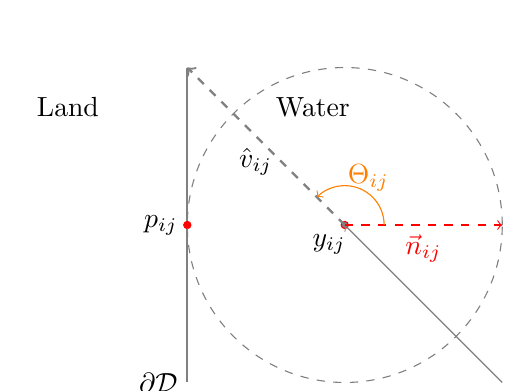
\begin{tikzpicture}
		%boundary
		\draw[gray, thick] (0,0) -- (0,4);
		%position
		\draw[red,fill=gray] (2,2) circle (.3ex);
		%nearest shore point
		\draw[red,fill=red] (0,2) circle (.3ex);
		%velocity
		\draw[->,gray] (4,0) -- (2,2);
		\draw[->,gray,dashed,thick] (2,2) coordinate (O) -- (0,4) coordinate (A);
		%normal vector
		\draw[->,red,dashed] (O) -- (4,2) coordinate (B);
		%trigonometric circle
		\draw[gray,dashed] (2,2) circle (2cm);
		%angle 
		\pic[draw=orange,->,angle eccentricity=1.2,angle radius=0.5cm] {angle=B--O--A};
		
		%nodes
		\node[left] at (-1,3.5) {Land};
		\node[right] at (1,3.5) {Water};
		\node[left] at (0,0) {$\partial \mathcal{D}$};
		\node[left] at (0,2) {$p_{ij}$};
		\node[left] at (1.2,2.8) {$\hat{v}_{ij}$};
		\node[below] at (1.8,2) {$y_{ij}$};
		\node[below,red] at (3,2) {$\vec{n}_{ij}$};
		\node[above,orange] at (2.3,2.3) {$\Theta_{ij}$};
	\end{tikzpicture}
	\caption{Example of nearest shore point and angle $\Theta$. $\partial D$ represents the boundary of the domain, $y_{ij}$ is the observed GPS position of narwhal $i$ at time $t_{ij}$.}
	\label{fig: illustration nearest shore points}
\end{figure}

\begin{comment}
	\begin{figure}[H]
		\centering
		\begin{subfigure}{0.48\textwidth}
			\centering
			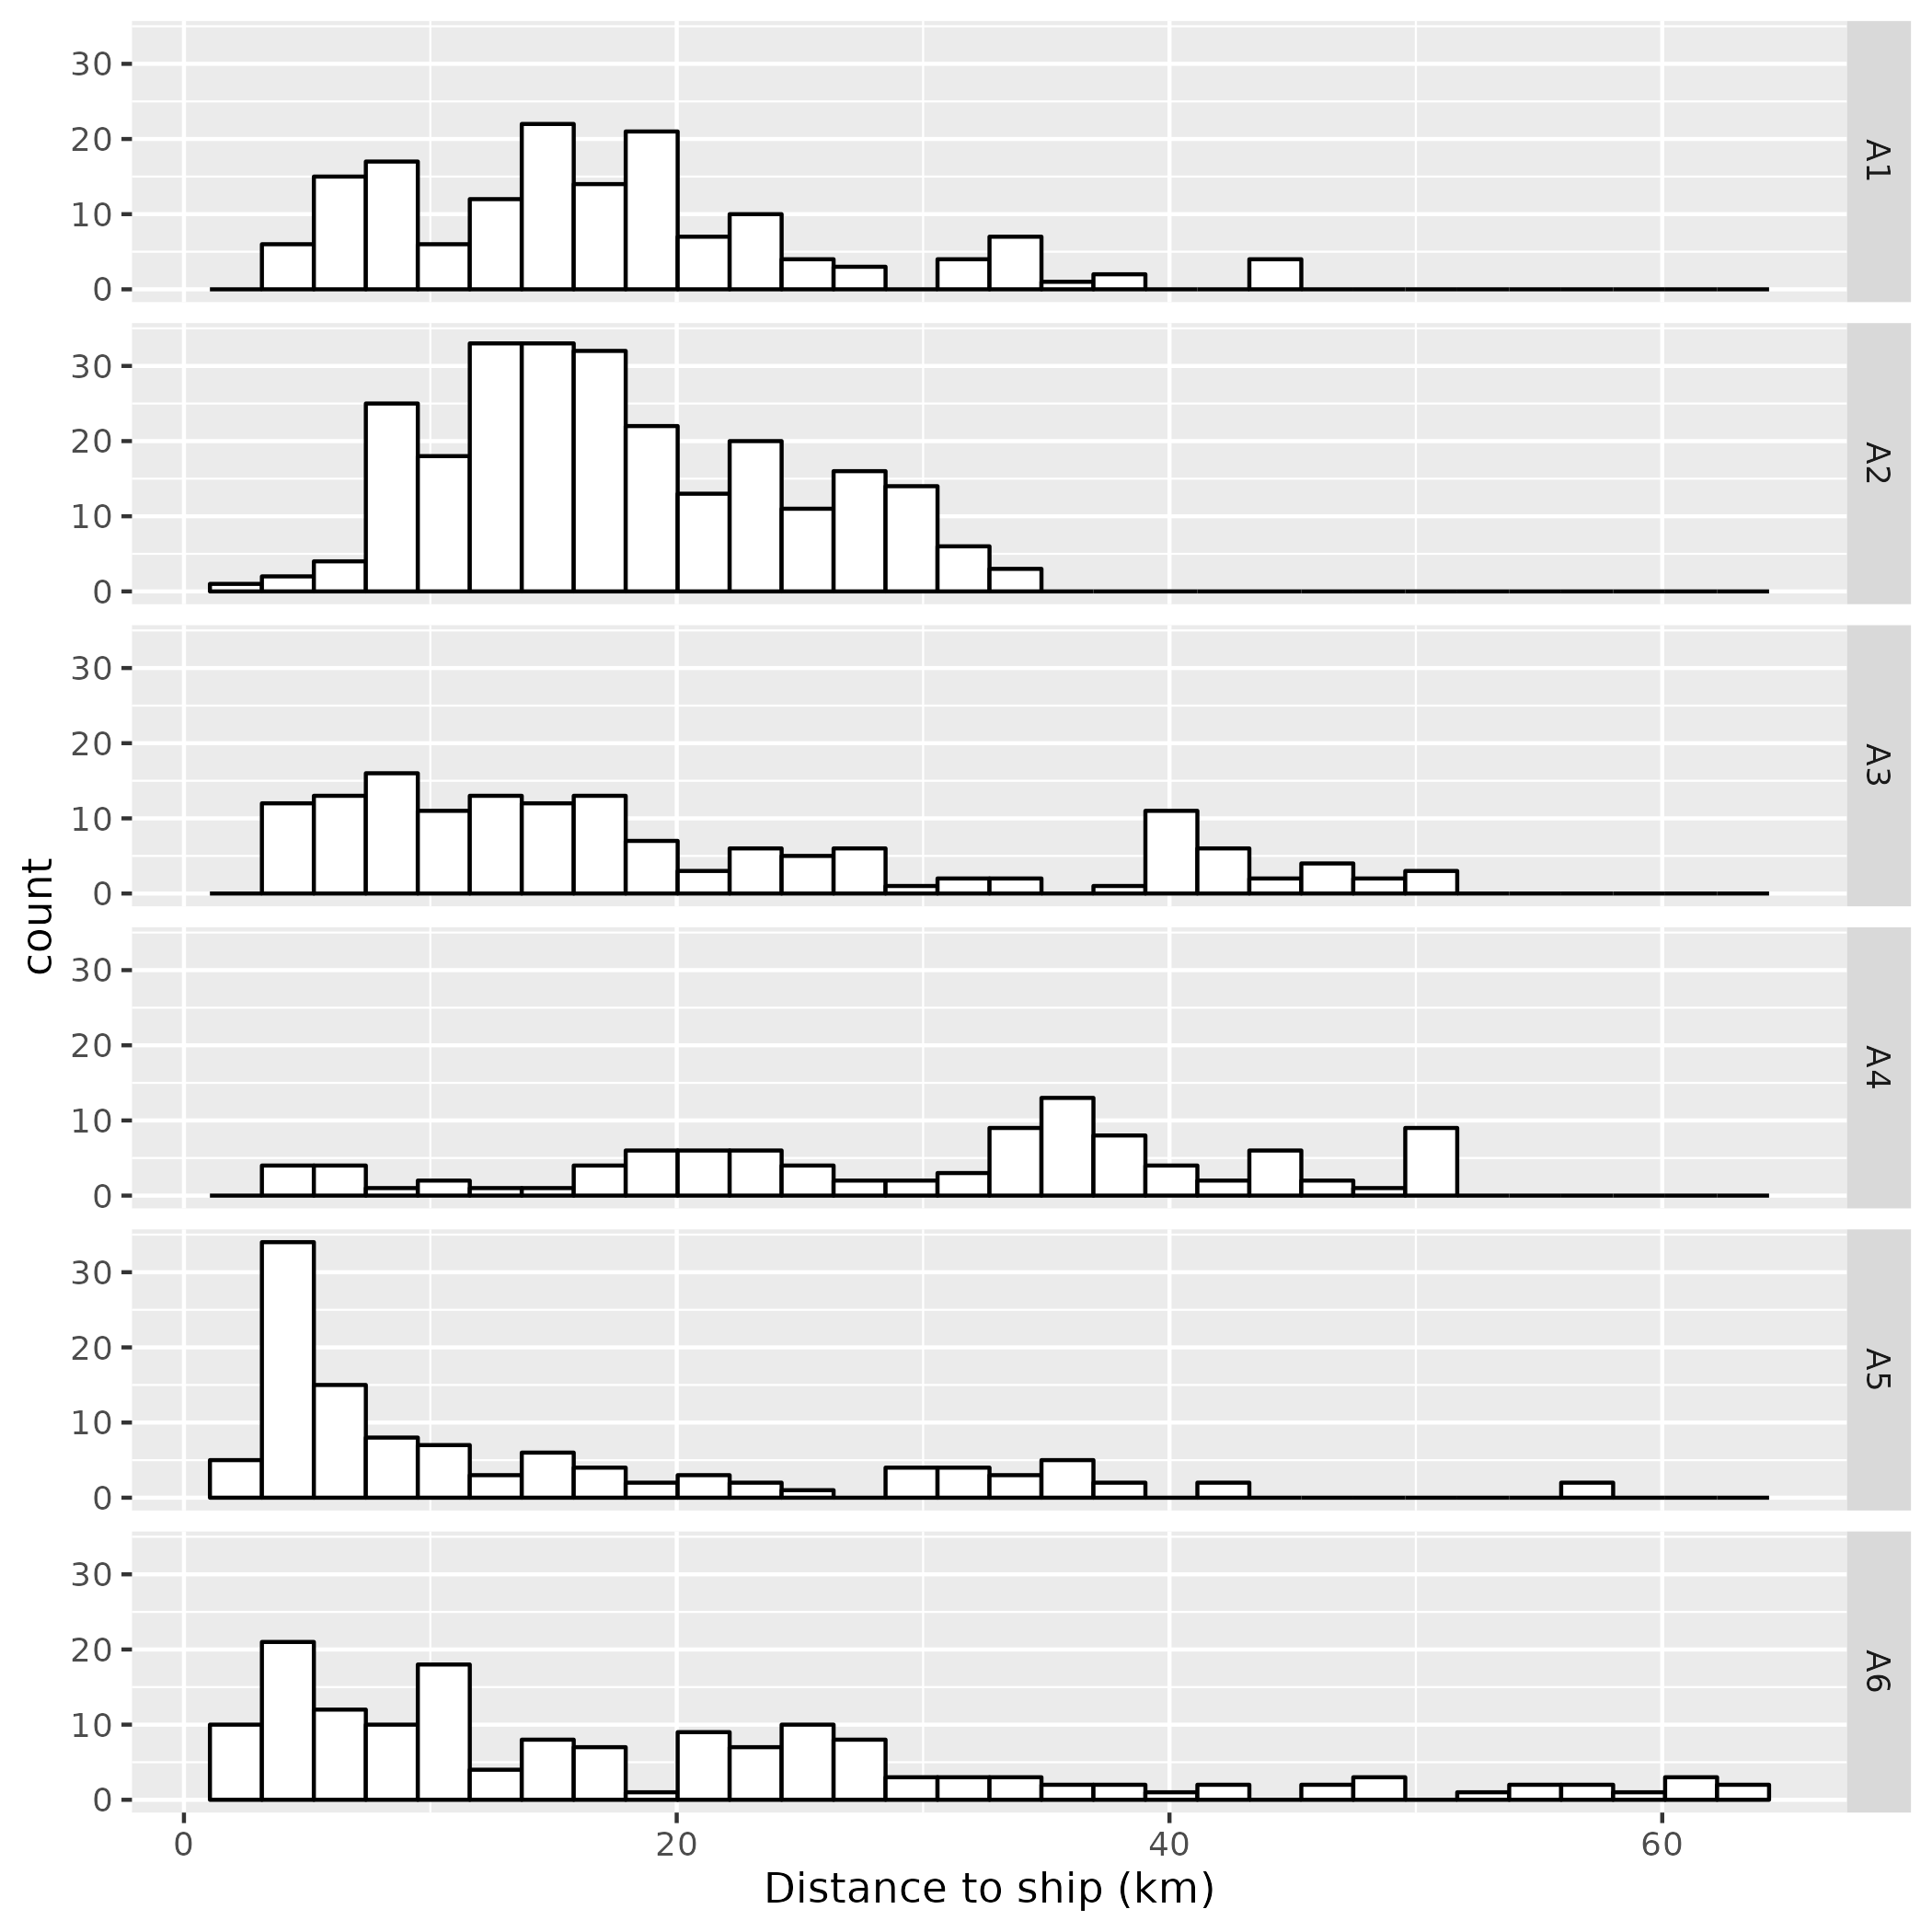
\includegraphics[scale=0.45]{images/data_exploration/Dship_histo.png}
			\caption{Histograms of the distance to the ship \\ for each narwhal}
		\end{subfigure}
		\begin{subfigure}{0.48\textwidth}
			\centering
			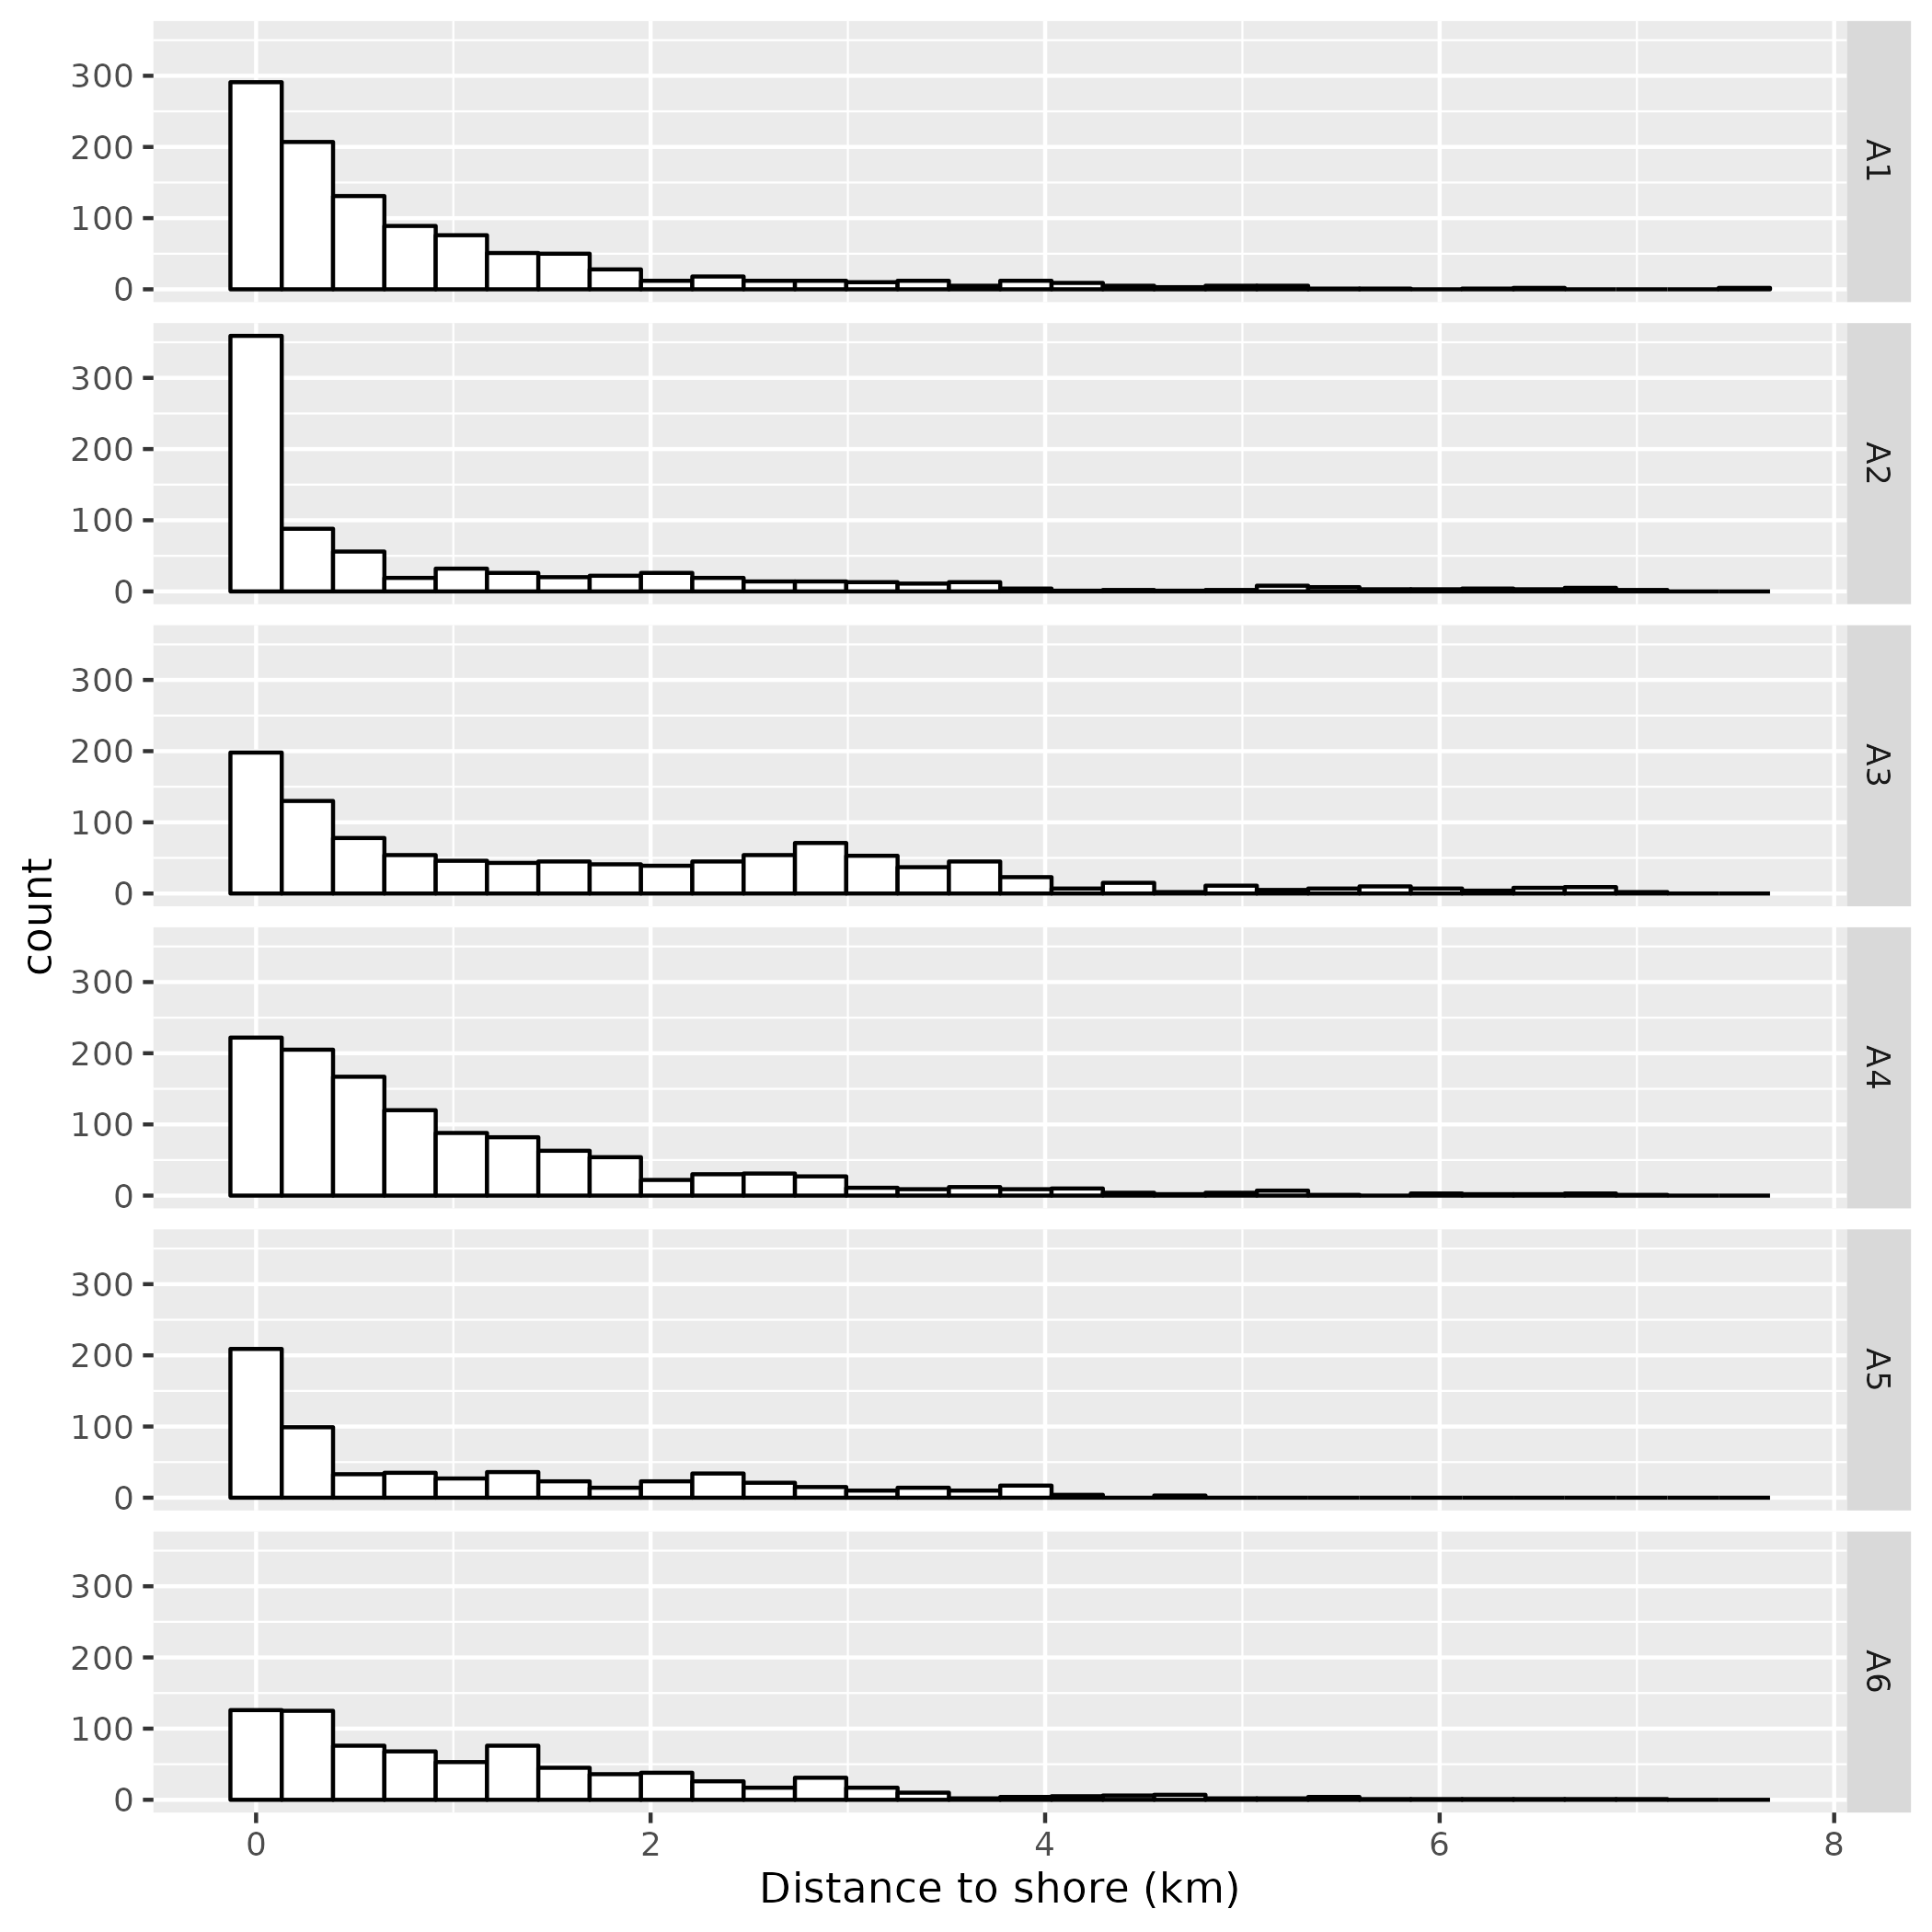
\includegraphics[scale=0.45]{images/data_exploration/Dshore_histo.png}
			\caption{Histograms of the distance to the shore \\ for each narwhal}
		\end{subfigure}
		\caption{Distance to ship and distance to shore covariates}
		\label{fig: distance to shore and distance to ship histograms}
	\end{figure}
\end{comment}

The distance from the ship denoted $D^{ship}_{ij}$, is estimated as the distance between the GPS ship and narwhals's positions. The values are comprised between $2.68$ and $63.8$ km.
Exposure to ship covariate for narwhal $i$ at time $t_{ij}$, denoted $E^{ship}_{ij}$, is defined as the inverse of the distance to the ship (in km) \cite{heide-jorgensen_behavioral_2021}.
$D^{ship}$ is only known when the narwhal is in line of sight with the boat, so that exposures are set to $0$ when this is not this case. This implies that the effect of the ship noise on the narwhals's movement is only considered in this specific case in the whole study, though it is very likely that narwhals can perceive the disturbance even when they are not clearly in line of sight with the sound source. This provides a conservative estimate of the effect of the noise exposure. The covariate $E^{ship}$ is meant to be a proxy for sound exposure levels received by the narwhals. Reasonably, the closer the narwhal is to the ship, the more it can hear its sound, and the greater the exposure. Exposure levels for each narwhals are displayed in figure~\ref{fig: realexpthroughtime}.


\begin{figure}[H]
	\centering
	\begin{subfigure}{0.48\textwidth}
		\centering
		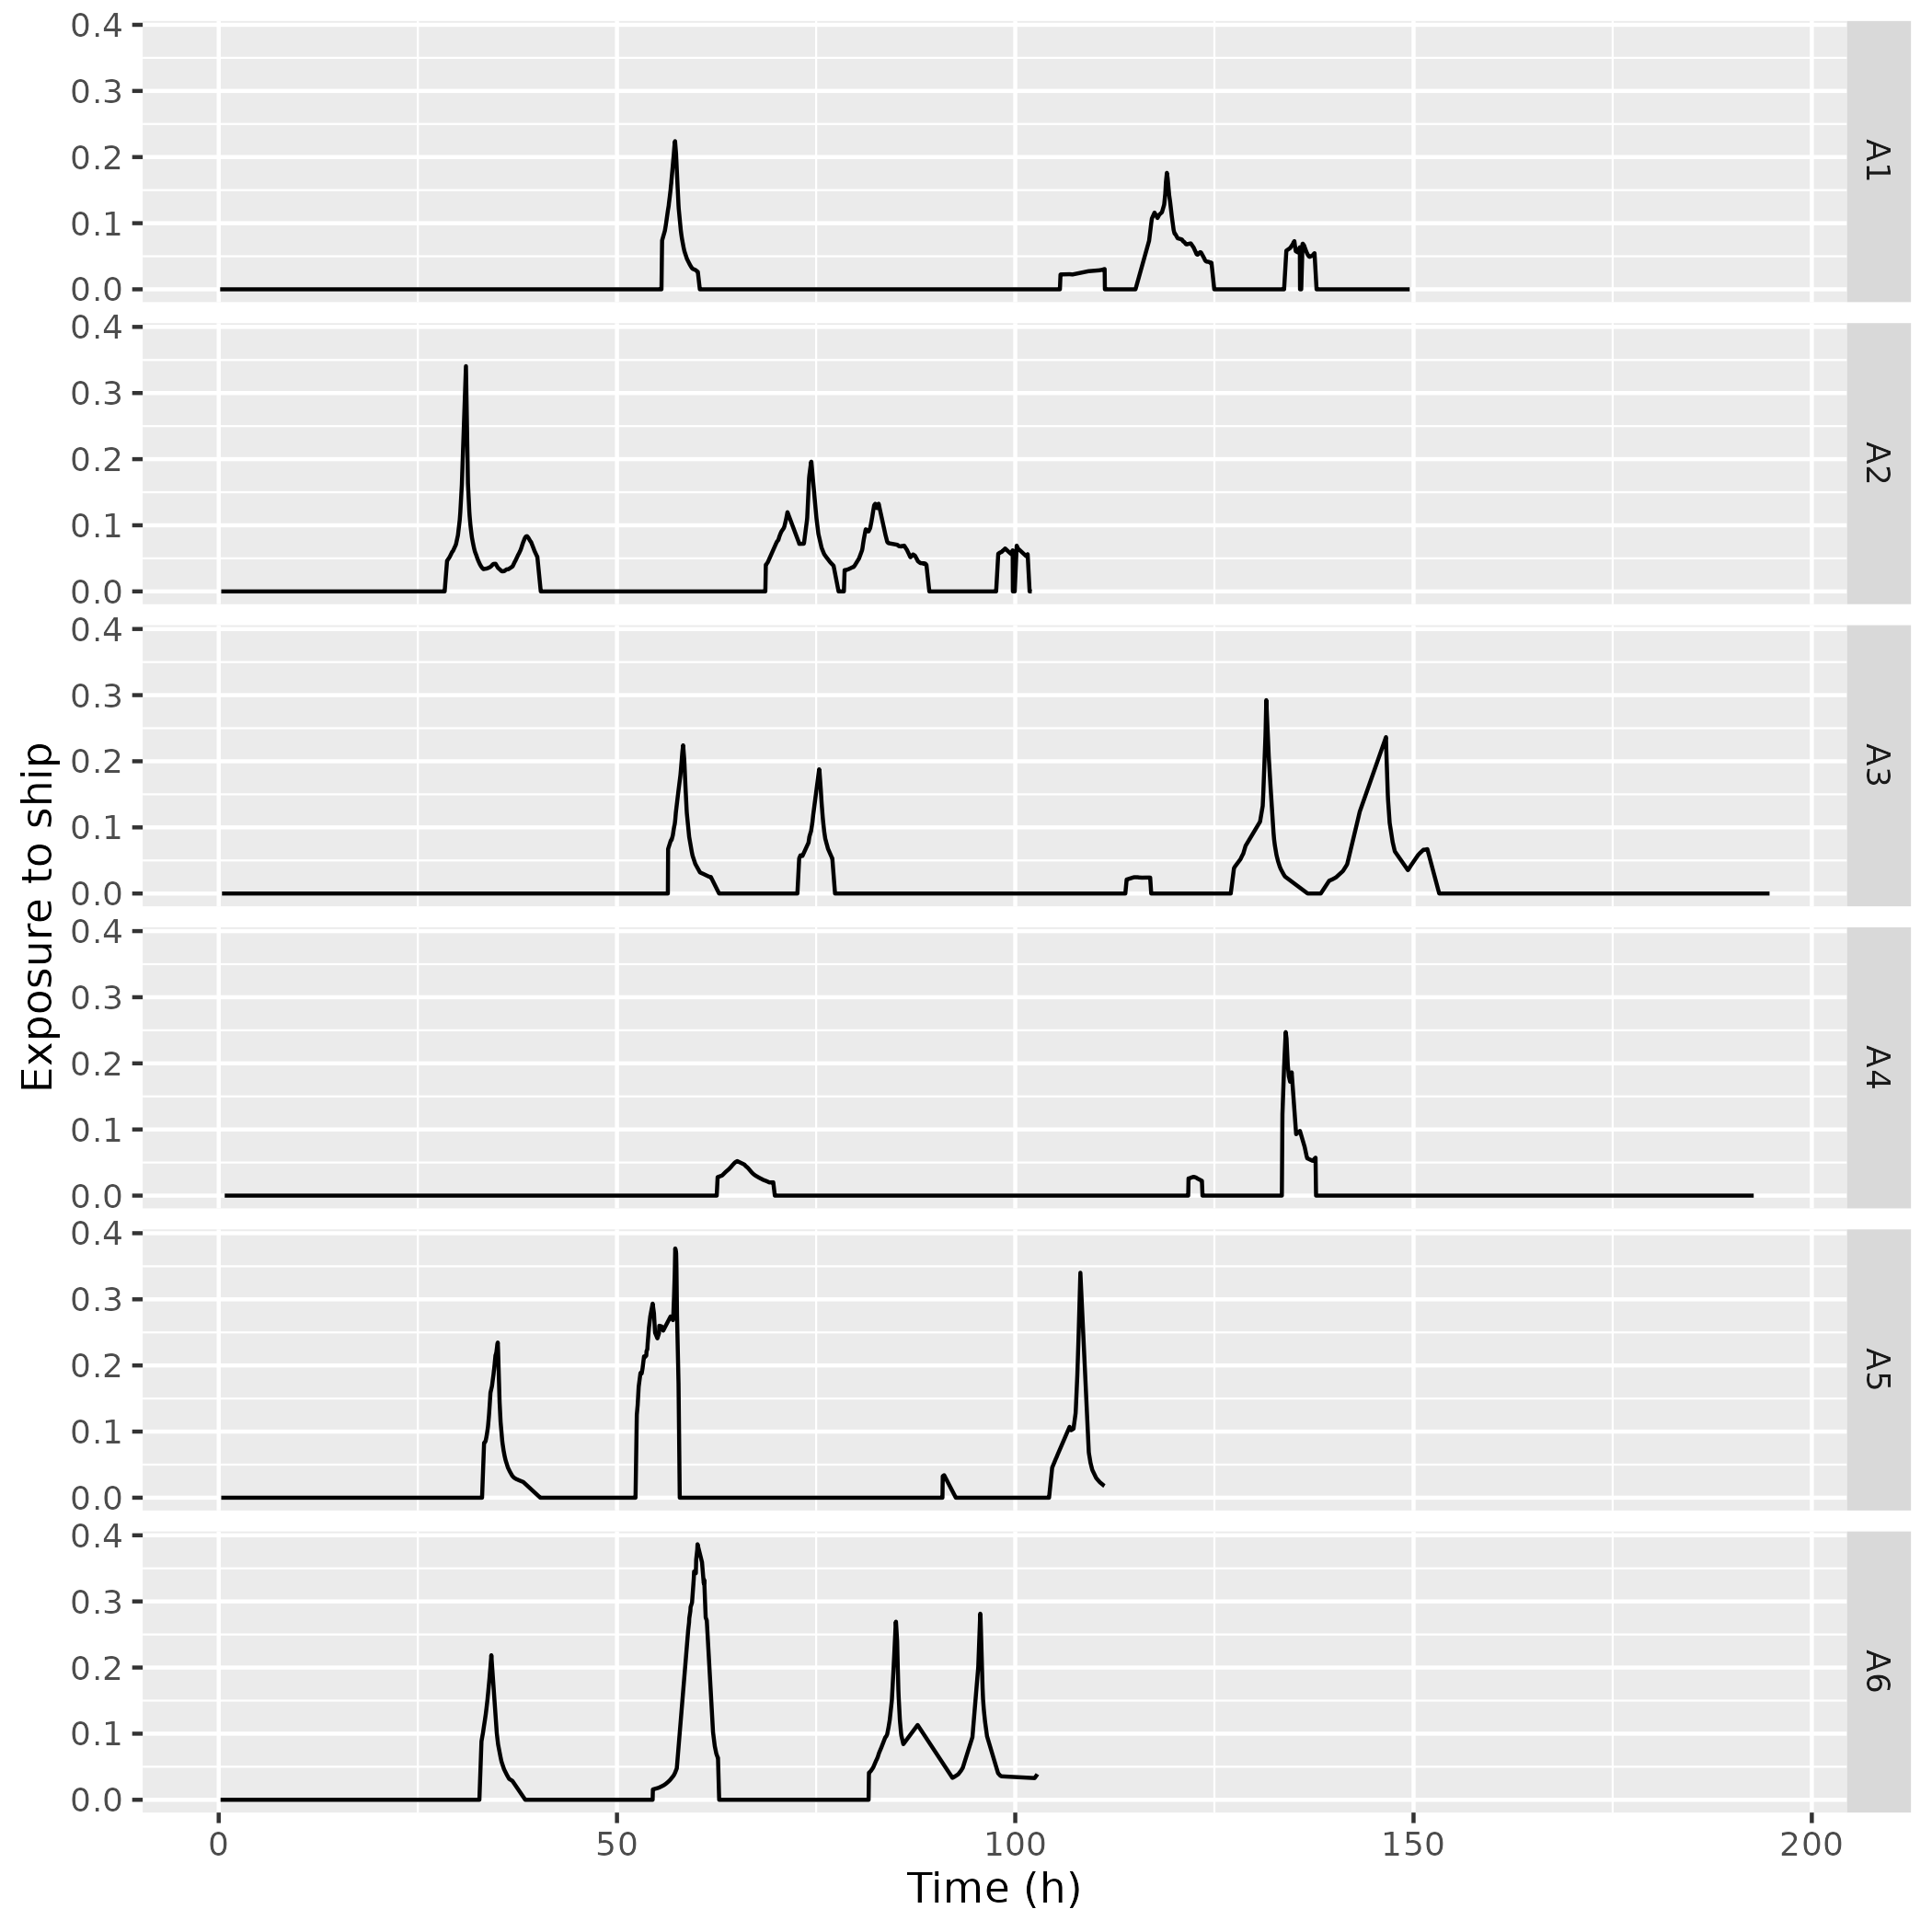
\includegraphics[scale=0.42]{images/data_exploration/realExpShip_through_time.png}
		\caption{}
	\end{subfigure}
	\begin{subfigure}{0.48\textwidth}
		\centering
		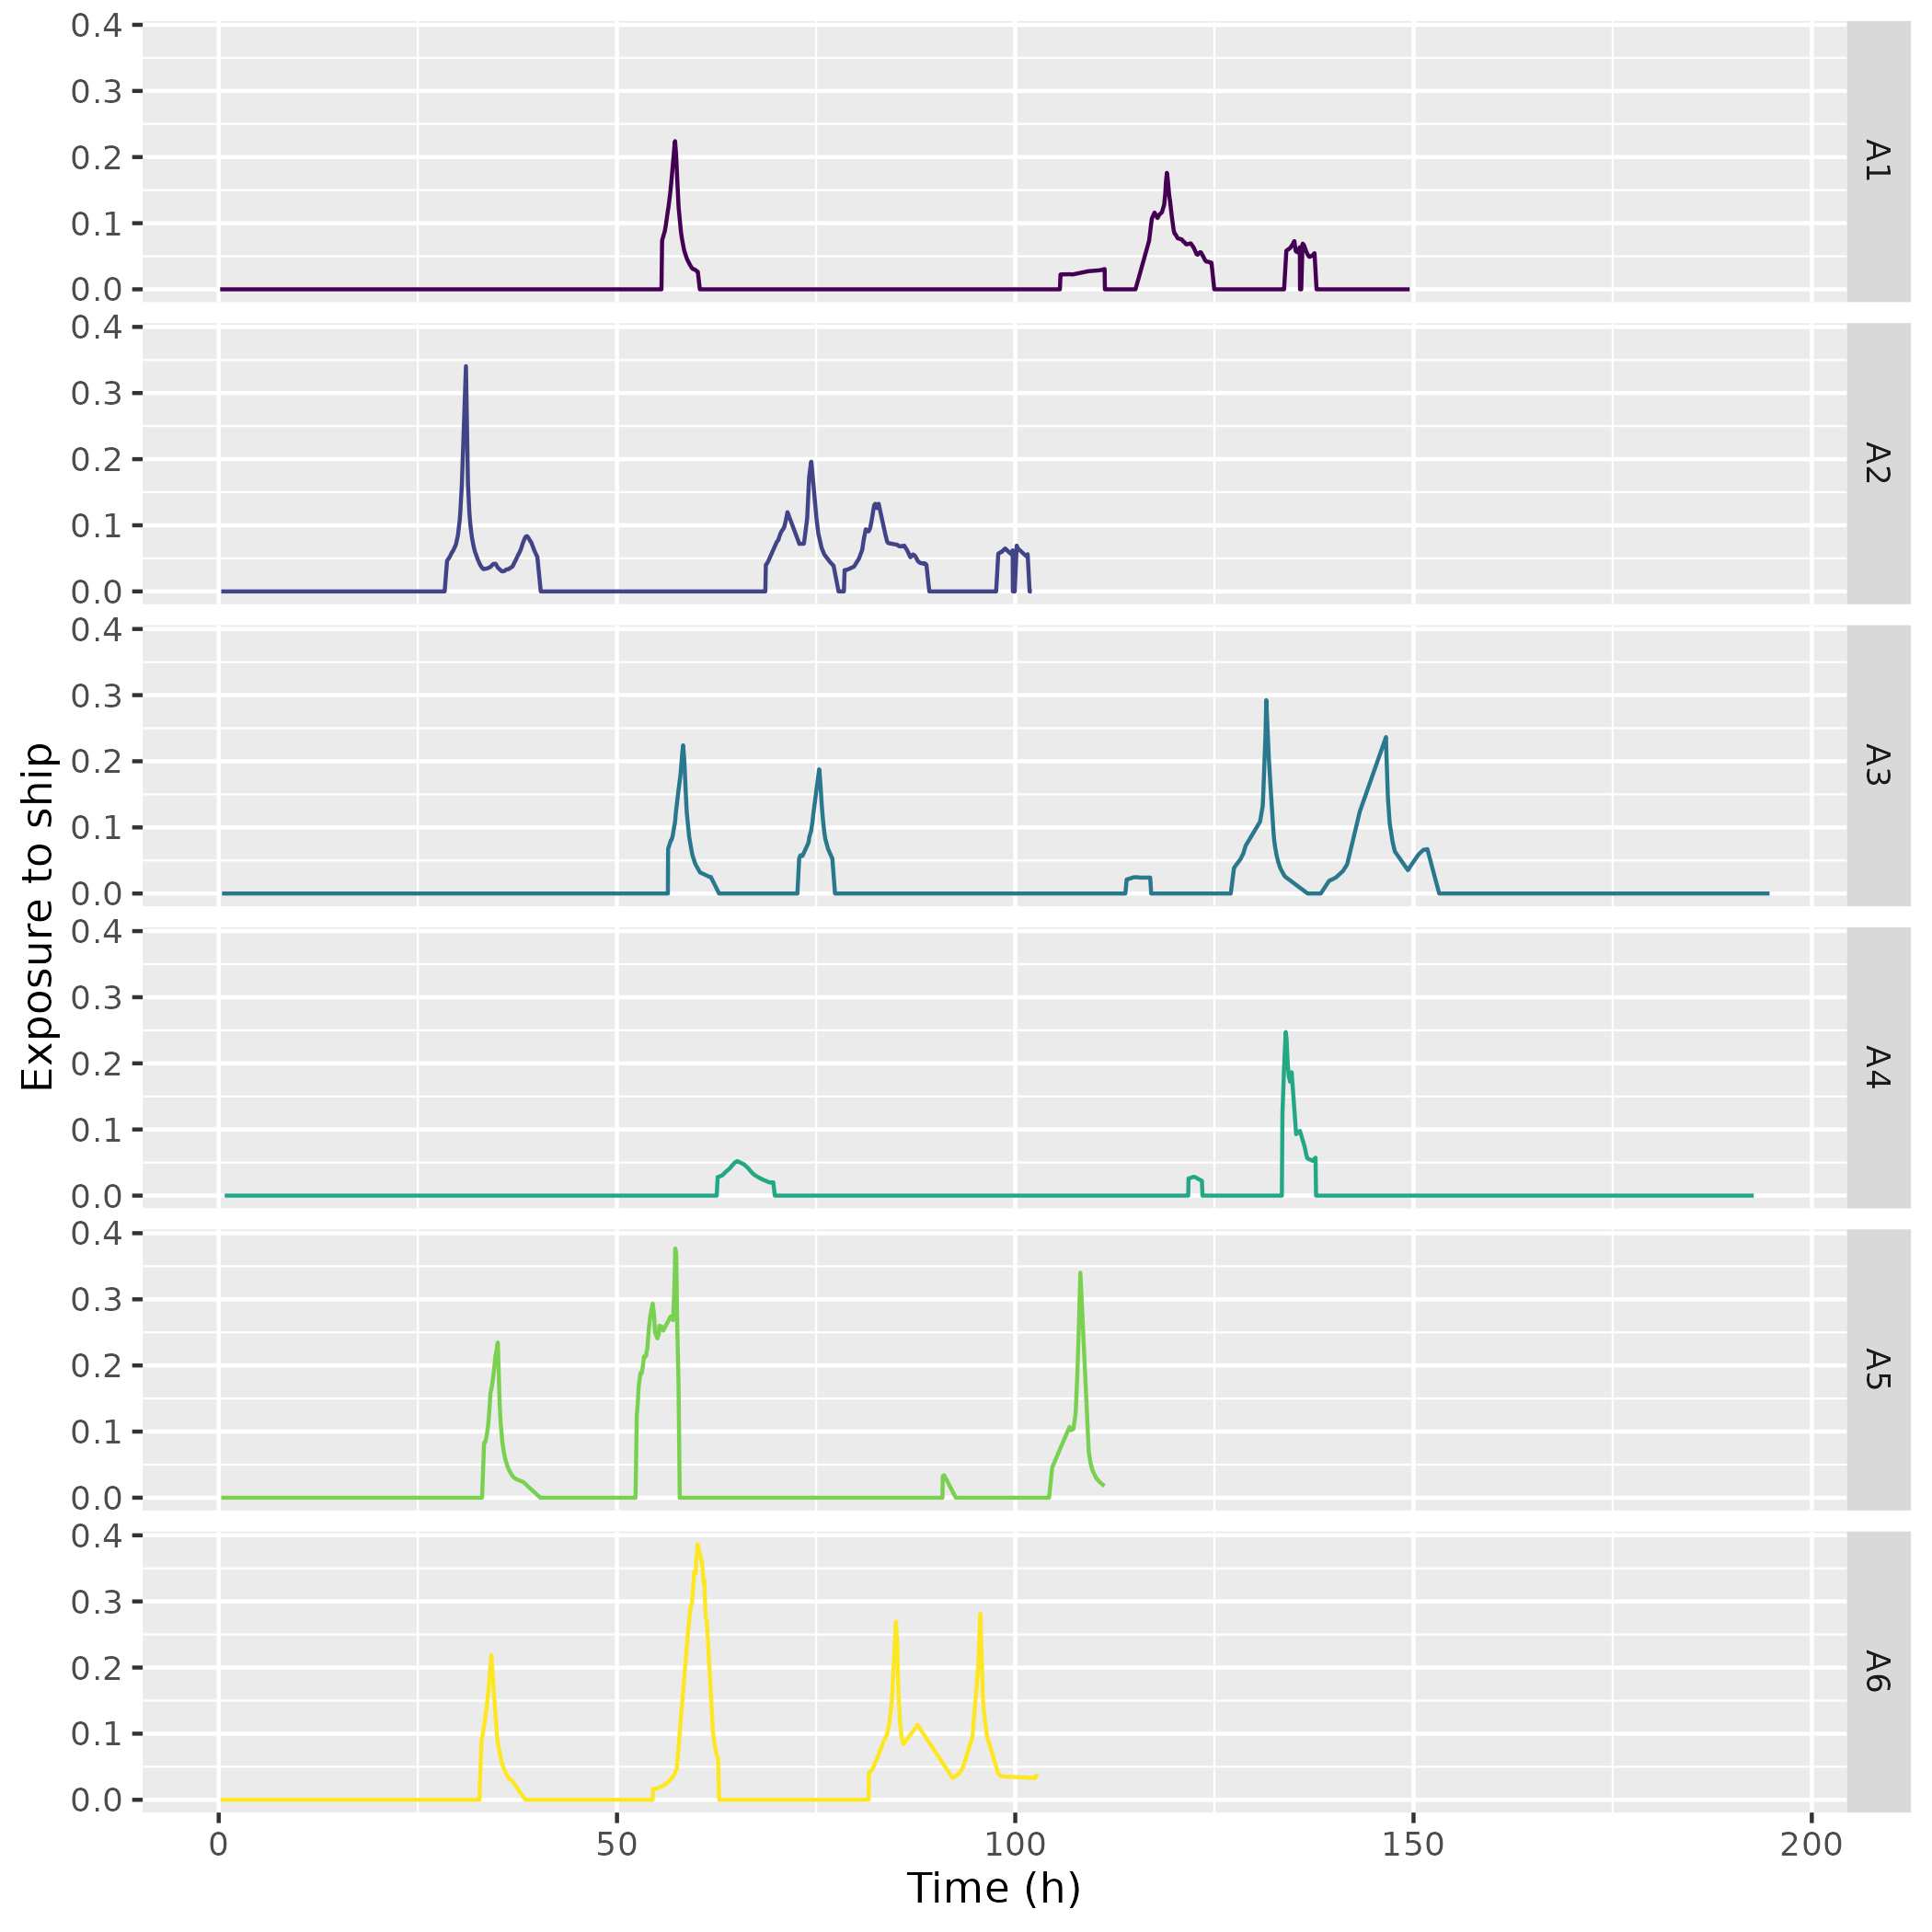
\includegraphics[scale=0.42]{images/data_exploration/realExpShore_through_time.png}
		\caption{}
	\end{subfigure}
	\caption{(a) Exposure to the ship (in $km^{-1}$) over time for each narwhal. (b) Exposure to the shore (in $km^{-1}$) over time for each narwhal.}  
	\label{fig: realexpthroughtime}
\end{figure}



\section{Diffusion models}

The dynamic of the true positions of the narwhals is controlled by a stochastic differential equation. First, we recall the standard diffusion model in this context, and then we modify it to include the effect of the shore on the movement and constrain the position within a polygon.


\subsection{Standard Rotational Advective correlated velocity model (RACVM)}
\label{section: RACVM}


We write $A=\begin{pmatrix} 
	\frac{1}{\tau} & -\omega \\
	\omega & \frac{1}{\tau}
\end{pmatrix}$ and recall equation~\ref{eq: RACVM equation}

\begin{equation*} \left\{
	\begin{array}{l}
		dX(t)=V(t)dt \\
		dV(t)=-A(V(t)-\mu)dt+\frac{2\nu}{\sqrt{\pi \tau}} dW(t) 
	\end{array}
	\right.
	\label{eq: RACVM equation bis}
\end{equation*}
where $X$ is the two-dimensional location and $V$ is the two-dimensional velocity.
In this section, we obtain explicit distributional results about the process $X$. Though this model is considered in several papers, we found no mention of the closed form formulas derived here. In \cite{gurarie_correlated_2017}, only the process $V$ is exhaustively studied, and the classical distributional results about this process are used for estimation and simulation purposes.
A more general formulation is considered by \cite{albertsen_generalizing_2018} in which the diffusion matrix is lower triangular matrix with positive diagonal elements whereas and two distinct autocorrelation parameters are considered in both directions allowing for anisotropic movement.
In this case, \cite{albertsen_generalizing_2018} derives an explicit form for the gaussian transition density of the velocity process, where the covariance matrix is expressed using a Kronecker sum \cite{albertsen_generalizing_2018}. But again, exact formulas for the process $X$ are not mentioned and the Euler-scheme is used to get approximate transition densities of $X$. Here, we claim that under the hypothesis of isotropic movement, with diagonal diffusion matrix as in equation ~\ref{eq: RACVM equation}, not only the velocity but also the position process have a closed form formula. \\


\begin{proposition}
	Let $U(t)=\begin{pmatrix} X(t) & V(t) \end{pmatrix}^\top$ for $t \geq 0$. Then the transition density of the Markov process $U$ is given by 
	\begin{equation}
		U(t+\Delta) \vert U(t)=u \sim \mathcal{N}\left( T(\Delta) u +B(\Delta)\mu, Q(\Delta)\right) \mbox{ for all } \Delta>0 \mbox{ and } u \in \R^4
		\label{eq: X V distribution}
	\end{equation}
where \begin{equation}
	T(\Delta)=\begin{pmatrix} I_2 & A^{-1}(I_2-\exp(-A\Delta)) \\
	0_2 & \exp(-A\Delta) \end{pmatrix} \mbox{ and } B(\Delta)=\begin{pmatrix}
	\Delta I_2 -A^{-1}(I_2-\exp(-A\Delta))\\
	I_2-\exp(-A\Delta)\end{pmatrix}
	\label{eq: link matrices}
	\end{equation}
and the covariance block matrix is given by
\begin{equation}
	Q(\Delta)=\begin{pmatrix}
		q_1(\Delta)I_2 & \Gamma(\Delta) \\
		\Gamma(\Delta)^\top & q_2(\Delta)I_2
	\end{pmatrix}
	\label{eq: covariance matrix}
\end{equation}
with 
\begin{equation}q_1(\Delta)=\frac{\sigma^2}{C}\left( \Delta-2 \frac{\omega \sin(\omega \Delta)-\frac{1}{\tau} \cos(\omega \Delta)}{C} \exp\left( -\frac{\Delta}{\tau} \right) +\frac{\tau}{2} \left( \frac{\omega^2-\frac{3}{\tau^2}}{C}-\exp\left( -\frac{2\Delta}{\tau}\right)\right) \right)
\end{equation}

\begin{equation}
	q_2(\Delta)=\frac{2\nu^2}{\pi}\left(1-e^{-\frac{2 \Delta}{\tau}}\right)
\end{equation}
\begin{equation}\Gamma(\Delta)=\begin{pmatrix} \gamma_1 & \gamma_2 \\
	-\gamma_2 & \gamma_1\end{pmatrix}
\end{equation}
where
\begin{equation}\gamma_1=\frac{\sigma^2}{2 C } \times \left( 1+\exp\left( -\frac{2\Delta}{\tau}\right)-2\exp\left( -\frac{\Delta}{\tau}\right) \cos(\omega\Delta)\right)
\end{equation}
\begin{equation}\gamma_2=\frac{\sigma^2}{C} \times\left( \exp\left( -\frac{\Delta}{\tau}\right) \sin(\omega \Delta)-\frac{\omega \tau}{2} \left(1-\exp\left( -2 \frac{\Delta}{\tau}\right) \right)\right)
\end{equation}
and we denoted $C=\frac{1}{\tau^2}+\omega^2$ and $\sigma=\frac{2\nu}{\sqrt{\pi \tau}}$.
\label{prop: transition density}
\end{proposition}

The formulas derived in \cite{johnson_continuoustime_2008} are a corollary of ~\ref{prop: transition density}, obtained with $\omega=0$. The proof of this proposition is detailed in Appendix.

Equation~\ref{eq: covariance matrix} shows that the two components of the location and velocity processes are independent.
Note that $\exp(-A\Delta)=e^{\frac{-\Delta}{\tau}} \begin{pmatrix} \cos(\omega \Delta) & \sin(\omega \Delta) \\ -\sin(\omega \Delta) & \cos(\omega \Delta) \end{pmatrix}$ is a weighted rotation matrix of angle $-\omega \Delta$.
Intuitively, ~\ref{eq: X V distribution} means that the next velocity $V(t+\Delta)$ is a weighted mean of the long term mean velocity $\mu$ and the previous velocity $V(t)$ rotated by an angle $-\omega \Delta$.
 Figure~\ref{fig: sample RACVM} shows one sample of a RCVM along with a sample of a constrained version of a RCVM that is defined in section~\ref{section: CRCVM}.\\


%samples with non zero and zero mu

\begin{figure}[H]
	\centering
	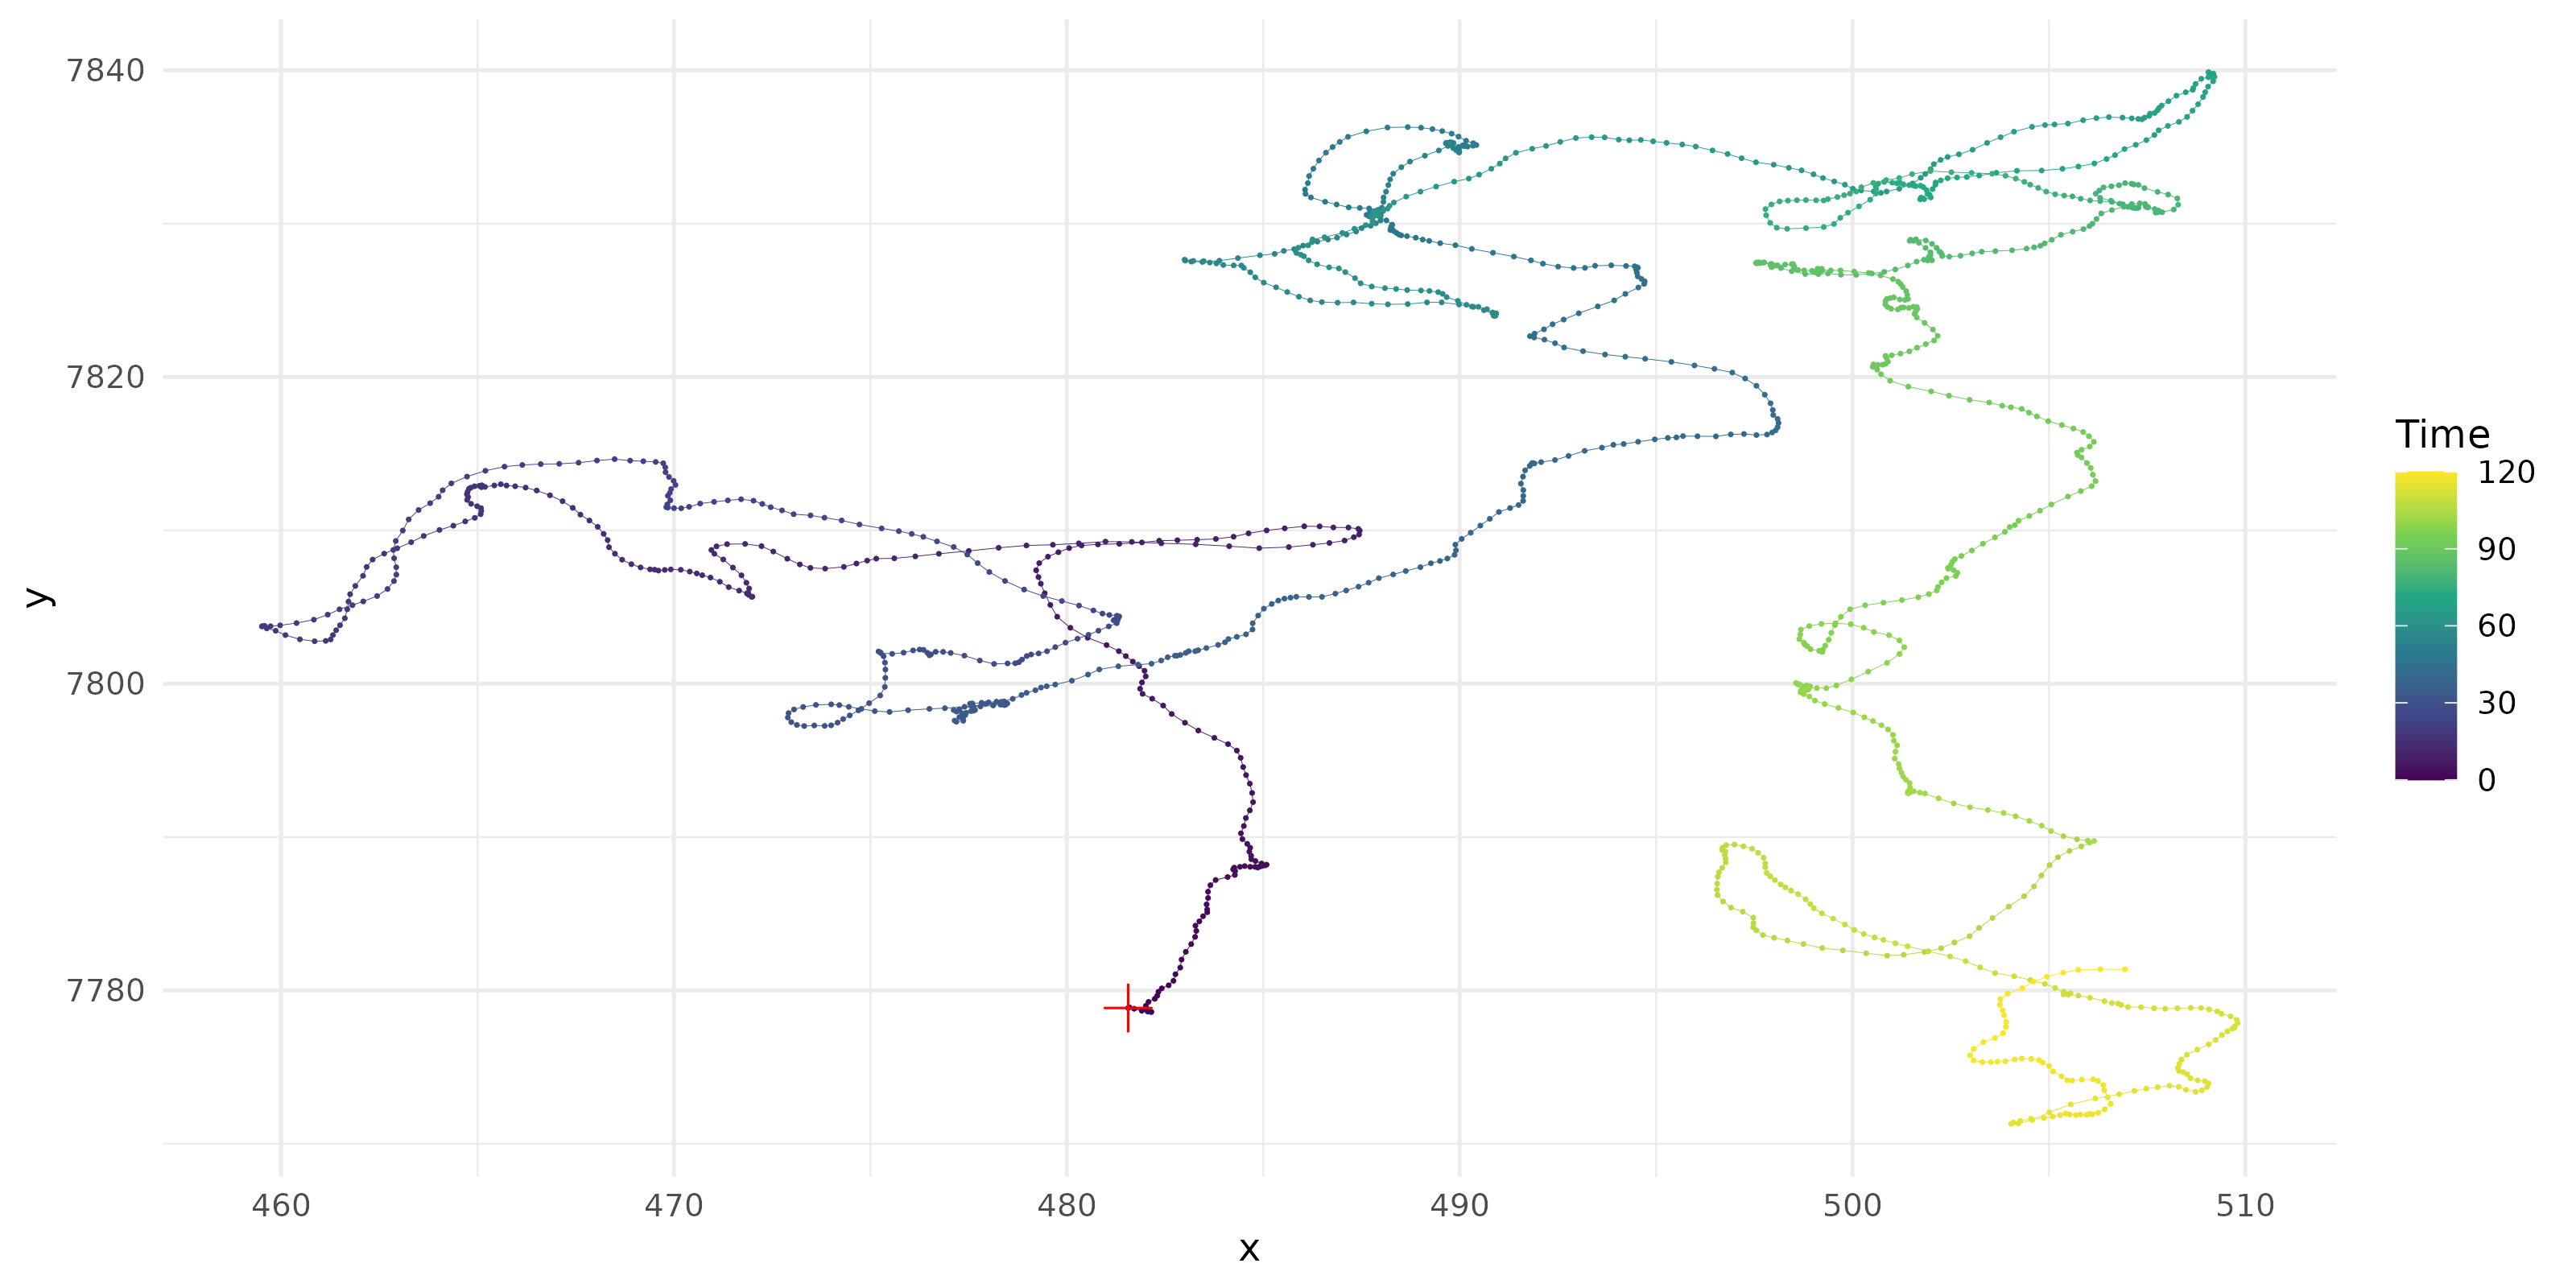
\includegraphics[scale=0.5]{images/rcvm/illustrative_sample_standard.png}
	\caption{Trajectory of a RCVM with parameters $\tau=1$h, $\nu=4$ km/h, $\omega=0.5$ rad/h, $\mu=(0,0)$ km/h and constant time step $\Delta=5$ min. The red cross indicates the starting point of the process. The samples were obtained from the exact transition density as derived in ~\ref{prop: transition density}.}
	\label{fig: sample RACVM}
\end{figure}


Unconstrained movement of marine mammals that do not exhibit a clear rotational movement, as it is often the case for marine mammals, is generally modeled through a CVM, that is equation~\ref{eq: RACVM equation} with $\omega=0$, while other animals or organisms whose motion appear tortuous require the more general model \ref{eq: RACVM equation}.
In the case of motion under spatial constraints, an increase in tortuosity enables the animals to avoid the boundary and adapt their heading to the constraint. 
\subsection{Constrained rotational correlated velocity model}
\label{section: CRCVM}

We thus propose to make use of a new RCVM that relies on the tortuosity parameter, or angular velocity $\omega$, to include how the animals turn in reaction to the shore. 
To do so, we introduce $\omega$ as a smooth function of the distance to the shore and the angle between the velocity vector and the shore normal vector. 
The smooth function should be non zero close to the shore, that is when a change of direction due to the proximity of the shore is expected, and  zero far away from the shore. 
We keep the notation $\mathcal{D} \subset \R^2$ for the polygon defining the domain of the process $X$. The new formulation of the equation is 
\begin{equation} \left\{
	\begin{array}{l}
		dX(t)=V(t) dt \\
		dV(t)=-A(X(t),V(t))V(t)dt+\frac{2\nu}{\sqrt{\pi \tau}} dW(t) 
		
	\end{array}
	\right.
	\label{eq: CRCVM equation}
\end{equation}

with 
\begin{equation} 
		A(X(t),V(t))=\begin{pmatrix} 
			\frac{1}{\tau} & -\omega(X(t),V(t)) \\
			\omega(X(t),V(t)) & \frac{1}{\tau}
		\end{pmatrix}
	\label{eq: CRCVM matrix A}
\end{equation}
where $\omega(X(t),V(t))=f_{\omega}(D^{shore}(t),\Theta(t))$, $D^{shore}(t)$ is the observed distance to the boundary of the domain $\partial \mathcal{D}$
and $\Theta(t)$ is the observed angle between the velocity $V(t)$ and the shoreline as defined in subsection ~\ref{subsection: covariates}. Thus, $f_{\omega}$ is a smooth function from $\R^{+} \times [-\pi,\pi]$ into $\R$.

Solving explicitly such a model is out of reach due to the non-linearity induced by the distance to the shore and the angle $\Theta$, but it is possible to get an approximate solution.
For any $t \geq 0$ and $\Delta>0$, if $\Delta$ is small enough, we can use the approximations
\[\forall s \in [t,t+\Delta], D^{shore}(s) \simeq D^{shore}(t) \quad \mbox{and} \quad  \Theta(s)\simeq \Theta(t)\]
In this case, we can use the formulas of section~\ref{section: RACVM} to get an approximation of the exact transition density.
The question still hanging is: what are the conditions on the function $f_{\omega}$ to ensure that the process is constrained ?
We don't formulate a comprehensive answer here, but only give examples of interpretable smooth functions that result in constrained samples of $X$.
An important spatial scale of the rotational movement is $\rho=\frac{\nu}{\omega}$, which is the diameter of rotation. It should always remain significantly lower than $D^{shore}$ for the process to be constrained. Moreover, a rotation needs to be considered near the boundary of the domain, that is when $D^{shore}$ approaches $0$, and when the narwhal is heading in the direction of the shore, that is for $\Theta \in \left[\frac{\pi}{2},\pi\right] \cup \left[-\pi,-\frac{\pi}{2}\right]$.
The closer we are to the shore, the faster the velocity should rotate,
whereas at a certain distance from the coast, there should be no further effect of the shore, meaning that $\omega$ should be close to $0$. Far from the coast, the movement model is simply an integrated Ornstein-Uhlenbeck process, as in the unconstrained case.
A weight based on the distance to the shore can be defined as follows :
\[c(D^{shore})=\exp\left(-\kappa \times \left(\frac{D^{shore}}{D_0}\right)^2\right)\mbox{ for some } D_0>0 \mbox{ and } \kappa>0\]

Based on this weight, a relationship between $f_{\omega}$ and the angle $\Theta$ and the distance to the shore $D^{shore}$ can be formulated  :

\begin{equation}
f_{\omega}(\Theta,D^{shore})=\frac{\omega_0}{2}\left(\tanh(\lambda(\theta+\theta^{*}))+\tanh(\lambda(\theta-\theta^{*})))\right)\times c(D^{shore})
\label{eq: smooth omega}
\end{equation}
for some $\omega_0 \in \R$, $\lambda>0$, $\theta^* \in [0,2\pi]$.

This parametrization of $\omega$ is only motivated by the observations above, and do not pretend to be optimal. Any smooth function that meets minimum requirements could be used instead. An alternative is to specify the smooth function $f_{\omega}$ using spline basis functions. Figures~\ref{fig: smoothomega1} and~\ref{fig: smoothomega2} show a smooth function obtained from equation~\ref{eq: smooth omega}, while figures~\ref{fig: smoothomegasplines1} and~\ref{fig: smoothomegasplines2}  represents a smooth function $f_{\omega}$ obtained as a combination of nine cubic spline basis functions. In the sequel, such models with $\omega$ as a smooth function of $D^{shore}$ and $\Theta$ meeting minimum requirements will be refered to as Constrained Rotational Correlated Velocity Models (CRCVM).

\begin{figure}[H]
	\centering
	\begin{subfigure}{0.48\textwidth}
		\centering
		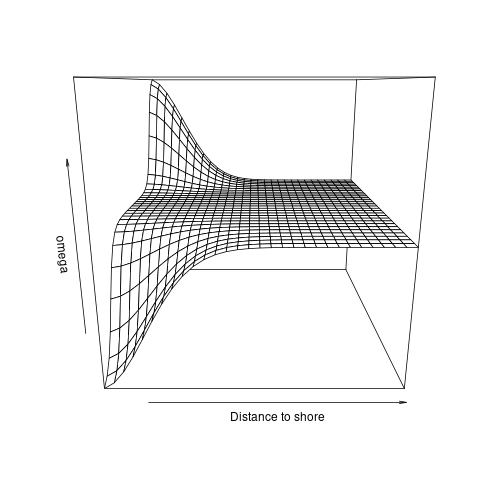
\includegraphics[scale=0.3]{images/crcvm/smooth_omega1.png}
		\caption{}
		\label{fig: smoothomega1}
	\end{subfigure}
	\begin{subfigure}{0.48\textwidth}
		\centering
		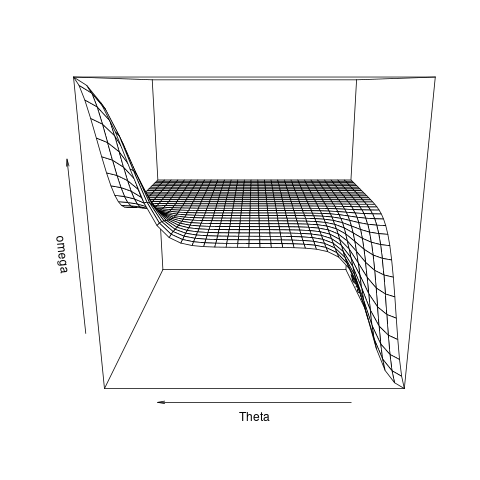
\includegraphics[scale=0.3]{images/crcvm/smooth_omega2.png}
		\caption{}
	\label{fig: smoothomega2}
	\end{subfigure}

	\begin{subfigure}{0.48\textwidth}
	\centering
	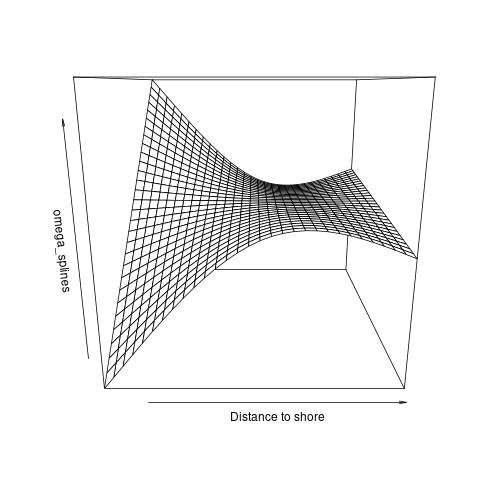
\includegraphics[scale=0.3]{images/crcvm/smooth_splines_omega1.png}
	\caption{}
	\label{fig: smoothomegasplines1}
	\end{subfigure}
	\begin{subfigure}{0.48\textwidth}
	\centering
	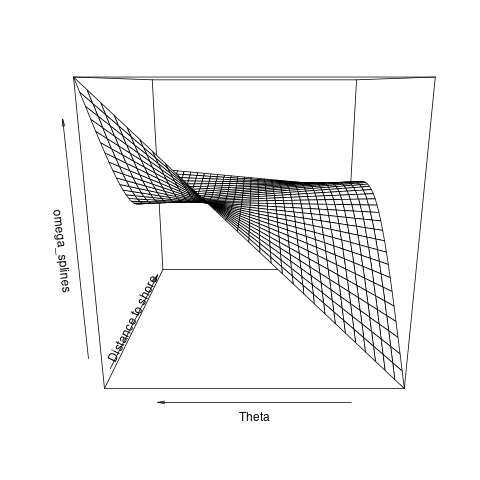
\includegraphics[scale=0.3]{images/crcvm/smooth_splines_omega2.png}
	\caption{}
	\label{fig: smoothomegasplines2}
	\end{subfigure}
	\caption{Examples of smooth functions $f_{\omega}$. Angular velocity $\omega$ increases as $\Theta$ approaches $\pm\pi$, and decreases with increasing distance to the shore. (a)-(b) Two views of the smooth function $f_{\omega}$ defined by equation~\ref{eq: smooth omega}. (c)-(d) Two views of a smooth function $f_{\omega}$ obtained by combining nine bivartiate cubic spline basis functions.}
	
\end{figure}



 This general model is very flexible, and different species-specific behaviours could be described. The function $\omega$ allows to control at which distance the animal will turn away from the shore, and how fast it will turn. We will show in section~\ref{section: simulation constrained motion} that is can be estimated from the observed positions, observed distances and angles. Specific constraints on the smooth function $f_{\omega}$ could also be set by biological expertise and knowledge about the species in question. Additionally, the tendency of an animal to move along the boundary of its spatial domain can be captured in the parameter $\tau$, as more persistent movement when the angle $\theta$ has value close to $\pm\frac{\pi}{2}$ would represent such an inclination. Again, this behavior can be statistically assessed from the observations. 
 
 More precisely, to model persistent movement along the shore line, we modify equation~\ref{eq: CRCVM matrix A} by expressing $\tau$ as a smooth function :
 \[\tau(X(t),V(t))=f_{\tau}(\Theta(t))\] where $f_{\tau}$ is a smooth function from $[-\pi,\pi]$ to $\R$.
 The function $f_{\tau}$ is defined such that it reaches local maximas in $\Theta=\pm\frac{\pi}{2}$, which represents movement along the boundary of the domain. An example of such a function is given in figure~\ref{fig:smoothtaubump}.
 \begin{figure}[H]
 	\centering
 	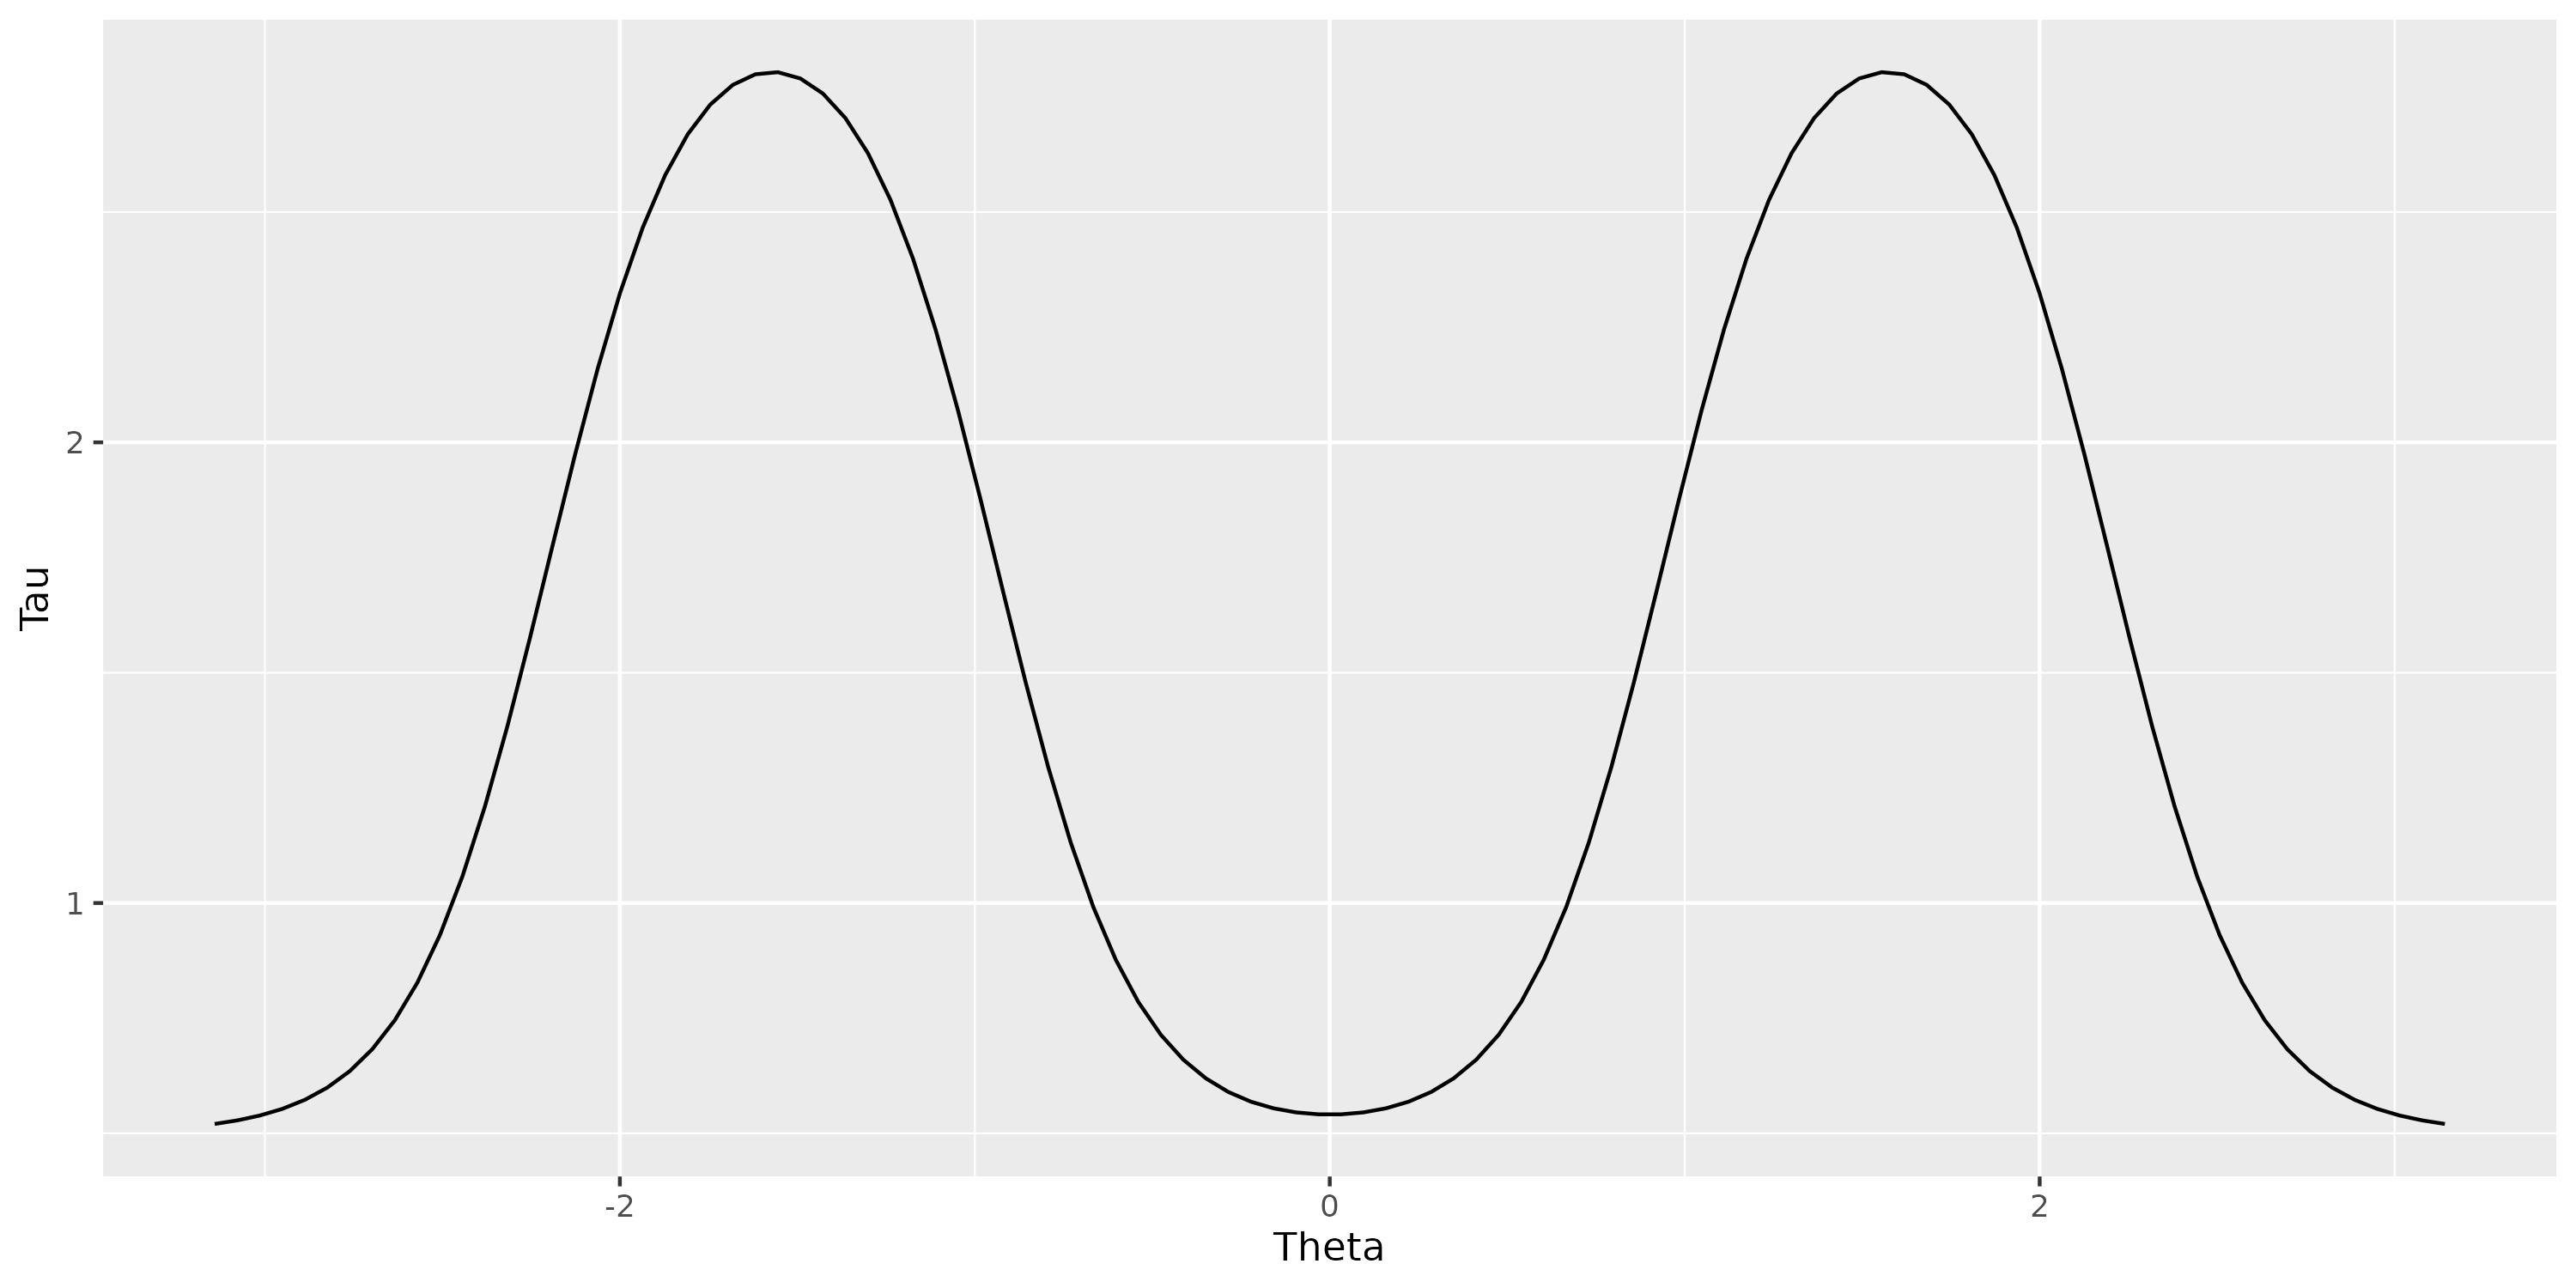
\includegraphics[scale=0.3]{images/crcvm/smooth_tau_bump}
 	\caption{Example of smooth function $f_{\tau}$ that can represent persistent movement along the boundary of the domain.}
 	\label{fig:smoothtaubump}
 \end{figure}
 
 We illustrate this flexibility in Figure~\ref{fig: crcvm examples}.Trajectories obtained within the fjords domain for different smooth functions $f_{\omega}$ and $f_{\tau}$ are shown side by side.
 
 \begin{figure}[H]
 
 	\begin{subfigure}{0.48\textwidth}
		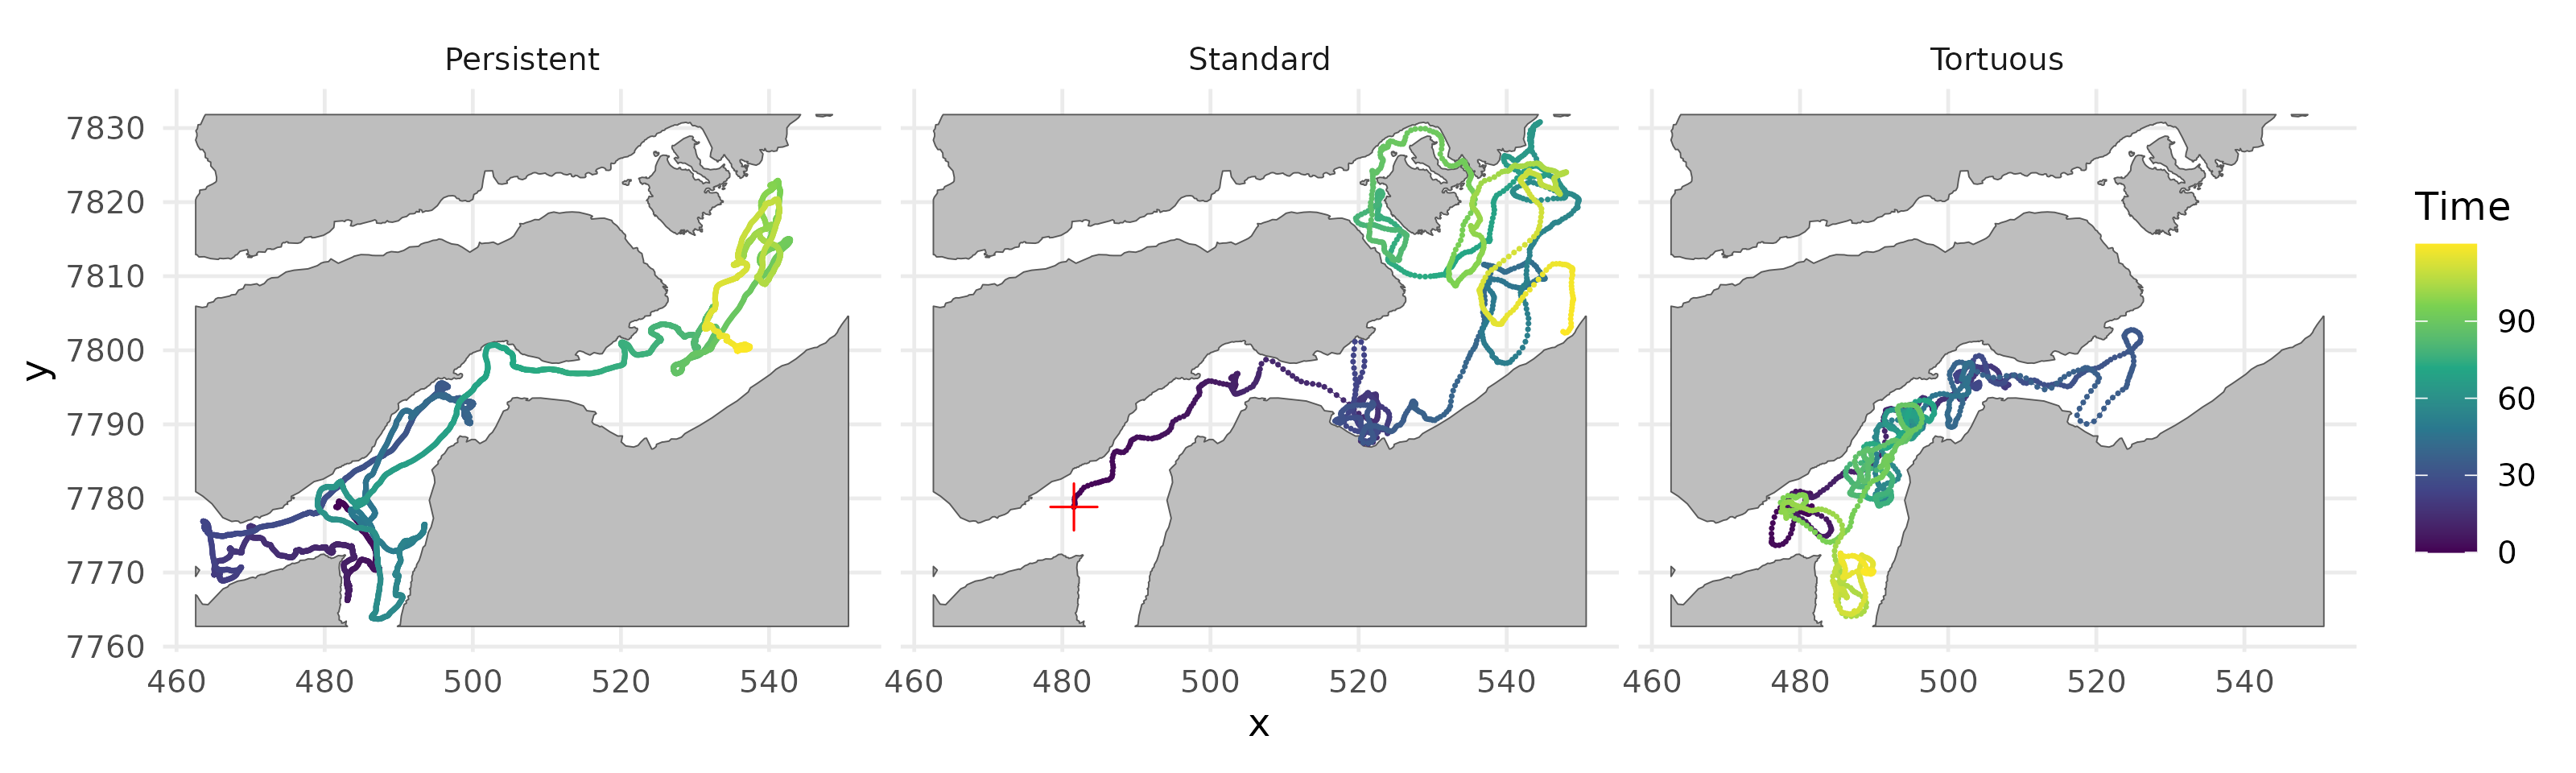
\includegraphics[scale=0.65]{images/crcvm/illustrative_sample_fjords}
		\label{fig:illustrativesamplefjords}
	\end{subfigure}


 	\caption{Five day trajectories with time step $\Delta=5$ min in Scoresby Sound fjords domain}
 	\label{fig: crcvm examples}
 \end{figure}




%discussion about tensor splines vs additive splines



\section{Inference of the sound exposure effect}


\subsection{Mixed effet model for sound exposure and shore effects}
\label{subsection: ship exposure effect}


%WHY TENSOR SPLINES : because covariates THeta and Eshore are not on the same scale, and identity link function
% FOR TAU: this makes sense to use additive splines since the link function is log
To assess if the exposure to the ship has a significative effect on the narwhals movement, a baseline model is first fitted only on the data before exposure, to get an estimation on how the narwhals move when they are not exposed to the disturbance. Then, a response model is fitted on the data during exposure and check whether the estimated smooth parameters deviate significatively from the baseline values. We present here the baseline and response models.\\

For the baseline model, only the effect of the shore is included through the shore exposure covariate $E^{shore}$ and the angle covariate $\Theta$.\\
Although individuals have a tendency to move in the same way, their movement don't have exactly the same characteristics depending on their age and size for instance. This is taken into account by using a mixed effect model for the RCVM parameters.
For each narwhal $i \in \{1, \cdots, N\}$, we have 	GPS observations $y_{ij}$ at times $t_{ij}$, $j \in \{1,\cdots,n_{i,pre}\}$ and the true motion processes $V_i$ and $X_i$ are supposed to solve equation~\ref{eq: CRCVM equation}. Because $\tau$ and $\nu$ can only be positive, a log link function is used for these parameters. The angular velocity $\omega$ is expressed as a smooth function of $\Theta$ and $E^{shore}$ through splines. Since both covariates are not on the same scale (one is in $rad$ while the other is in $km^{-1}$), tensor splines were judged more appropriate than thin plate regression splines \cite{wood_generalized_2017}.\\

Denoting $n_{i,pre}$ the number of observations before exposure for the narwhal $i$, and $\tau_i$, $\nu_i$, $\omega_i$ the parameters of the diffusion. The complete statistical model for the baseline estimations is the following:

\begin{equation}  \forall i \in \{1,\cdots,N\}, \quad \left\{
	\begin{array}{l}
		y_{ij}=X_{ij}+\varepsilon_{ij} \quad j \in \{1,\cdots,n_{i,pre}\}\\
		\varepsilon_{ij} \underset{i.i.d}{\sim} \mathcal{N}(0,\sigma_{obs}^2)  \\
		dX_i(t)=V_i(t)dt  \\
		dV_i(t)=-\begin{pmatrix} 
			\frac{1}{\tau_i} & -\omega_i(t) \\
			\omega_i(t) & \frac{1}{\tau_i}
		\end{pmatrix}V_i(t)dt+\frac{2\nu_i}{\sqrt{\pi \tau_i}} dW(t) \\
		\log(\tau_i)=\log(\tau_0)+b_{\tau,i}\\
		\log(\nu_i)=\log(\nu_0)+b_{\nu,i}  \\
		\begin{pmatrix} b_{\tau,i} \\ b_{\nu,i} \end{pmatrix} \underset{i.i.d}{\sim} \mathcal{N}\left(0,\begin{pmatrix} \sigma_{\tau}^2 & 0 \\ 0 & \sigma_{\nu}^2 \end{pmatrix}\right) \\
		\omega_i(t)=\omega_{0}+\sum_{k=1}^{L} \omega_{k} \psi_k(E_i^{shore},\Theta_i)
	\end{array}
	\right.
	\label{eq: exact baseline model}
\end{equation}



The coefficients $\log(\tau_{0})$, $\log(\nu_{0})$, $\omega_{0}$ are population intercepts and $b_{\tau,i}$, $b_{\nu,i}$
are the individual parameters. 

The functions $\psi_k$ in equation~\ref{eq: exact baseline model} are bivariate basis functions constructed through tensor products of univariate cubic spline basis functions. We refer to \cite{wood_generalized_2017} section $4.
1.8$ for the construction of tensor splines basis functions. The splines degree of freedom is $L=q_E \times q_{\Theta}$ and the numbers of knots in the splines is $q_E-1$ and $q_{\Theta}-1$ for the respective covariates $E_{shore}$ and $\Theta$. It is needed to choose them before hand.\\

Then, the response model is designed to assess a deviation from the baseline model due to exposure to the ship. We illustrate this by addding a dependency on the covariate $E_{ship}$ in the parameters $\tau$ and $\nu$. 
For $i \in \{1, \cdots, N\}$, denote $n_{i,post}$ the number of post-exposure observations for the narwhal $i$.

\begin{equation}   \left\{
	\begin{array}{l}
		y_{ij}=X_{ij}+\varepsilon_{ij}, \quad j \in \{1,\cdots,n_{i,post}\} \\
		\log(\tau_{i}(t))=\log(\tau_{0}) +\sum_{k=1}^{q} \log(\tau_{k})\phi_{k}(E^{ship}_i(t))+b_{\tau,i} \\
		\log(\nu_{i}(t))=\log(\nu_{0}) +  \sum_{k=1}^{q} \log(\nu_{k}) \phi_{k}(E^{ship}_i(t)) +b_{\nu,i}  \\
	\end{array}
	\right.
	\label{eq: exact response model}
\end{equation}

The intercepts $\log(\tau_0)$, $\log(\nu_0)$ and the spline coefficients $\omega_k$, $k \in \{1,\cdots,L\}$ are considered are offset.
The functions $\phi_k$ are cubic spline basis functions and $q$ is the spline degree of freedom for the exposure to the ship covariate. Only the parameters $\log(\tau_k)$ and $\log(\nu_k)$ are estimated from the trajectories during exposure to the sound





\subsection{State-space model}
\label{section: state space model}
In most applications, the error between the observation $Y$ and the true position $X$ is not negligible, so that it is needed to consider measurement errors through a state-space model as done by \cite{johnson_continuoustime_2008}. This is the approach we use here. In the statistical model~\ref{eq: exact baseline model} for the baseline model, we make the approximation mentioned in \cite{michelot_varying-coefficient_2021} that the parameter $\omega_i$ is constant on each time step $[t_{ij},t_{i,j+1}]$, equal to its value at time $t_{ij}$, that is 
\[\forall t \in [t_{ij},t_{i,j+1}], \quad \omega_{i}(t) \simeq \omega(t_{ij})= f_{\omega}(E^{shore}_{ij},\Theta_{ij})\]
 Denote $\Delta_{ij}=t_{i,j+1}-t_{ij}$, $V_{ij}=V(t_{ij})$, $X_{ij}=X(t_{ij})$, ,$\omega_{ij}=\omega(t_{ij})$, $A_{ij}=\begin{pmatrix} 
	\frac{1}{\tau_{i}} & -\omega_{ij} \\
	\omega_{ij} & \frac{1}{\tau_{i}}
\end{pmatrix}$ and $U_{ij}=\begin{pmatrix} X_{ij,1}  & X_{ij,2} & V_{ij,1} & V_{ij,2}\end{pmatrix}^\top$ where $\log(\tau_i)=\log(\tau_0)+b_{\tau}^{(i)}$ and $\log(\nu_i)=\log(\nu_0)+b_{\nu}^{(i)}$.

Discretisation of~\ref{eq: X V distribution} gives the following state-space equations:

\begin{equation}
	\forall i \in \{1,\cdots,N\}, \left\{
	\begin{array}{l}
		y_{ij}=ZU_{ij}+\varepsilon_{ij} \quad j \in \{1,\cdots,n_i\}\\
		\varepsilon_{ij} \underset{i.i.d}{\sim} \mathcal{N}(0,\sigma_{obs}) \\
		U_{i,j+1}=T_{ij} U_{ij} + \eta_{ij} \\
		\eta_{ij} \sim \mathcal{N}(0,Q_{ij})
	\end{array}
	\right.
	\label{eq: RACVM state space}
\end{equation}
where $Z=\begin{pmatrix} I_2 & 0_{2,2}\end{pmatrix}$, the link matrices $T_{ij}$ and $B_{ij}$ are computed according to~\ref{eq: link matrices} and the covariance matrix is computed according to~\ref{eq: covariance matrix}.
\\

Estimation with $\texttt{smoothSDE}$ relies on this state-space formulation in section~\ref{section: state space model} with the approximation that the parameters are constant on each time step between consecutive observations.
The complete likelihood is computed from the observations $y_{ij}$ as a by-product of the Kalman filter algorithm \cite{michelot_varying-coefficient_2021}.
Laplace's approximation of the integral of this complete likelihood over the random effects is computed using the \texttt{R} package \texttt{TMB}  and optimization is performed via the \texttt{optim} function in $\texttt{R}$ with the BFGS gradient method, with the gradient being calculated by automatic differenciation. We refer to \cite{kristensen_tmb_2016} for more details about the derivation of the multidimensional Laplace's approximation and the gradient computations. Similarly, we refer to \cite{wood_generalized_2017} section $6.6$ for the specification of the mixed effect model for the parameter of the SDE and the regularization terms that are based on a wiggliness measure involving gaussian priors for the spline coefficients $\omega_k$, $k \in \{1,\cdots,L\}$. \\
This is the technique is already available for the CVM, which corresponds to the special case $\omega=0$. Here, we extend this inference method to the more general model~\ref{eq: CRCVM equation} and use it for estimation of the baseline and the response models~\ref{eq: exact baseline model},~\ref{eq: exact response model}.




\section{Simulation study for the baseline model}
\label{section: simulation constrained motion}
In order to experiment the constrained models we simulate a CRCVM within different domains for smooth parameters $\omega$ depending on the angle $\Theta$ and the distance to the boundary of the domain. We consider observations of a baseline model as described in equation~\ref{eq: exact baseline model}.\\


We simulate $M=100$ batches of $N=6$ individual trajectories over $T=24$ h with time step $\Delta=1$ min in Scoresby Sound fjords system in which the narwhals move under constraints in our application.. This amounts to $n_{i,pre}=1440$ observations for each individual $i \in \{1,\cdots,N\}$. We fix $\sigma_{obs}=5$ m to represent low measurement errors. 
We choose $L=8$ for the degree of freedom of the bivariate splines of $E^{shore}$ and $\Theta$. The random effects standard deviations are set to $\sigma_{\tau}=0.2$ and $\sigma_{\nu,pre}=0.1$ to represent the individual variability, and $\tau_{0}$ and $\nu_{0}$ are fixed respectively to $1$ h and $4$ km/h. The exact values of the spline coefficients $\omega_k$, $k \in \{0,\cdots,L\}$ used to simulate the trajectories are given in Table~\ref{table: estimation performance fjords 12h}. For each trajectory, initial velocity is set to $(0,0)$ and initial position is uniformly sampled in the rectangular domain, at least $1$ km away from the boundary. We kept the same $6$ initial positions for all the batches of trajectories. To obtain the trajectories of the CRCVM, we suppose that the value of the parameter $\omega$ is constant on each time step. The next position and velocity are then obtained from equation~\ref{eq: RACVM state space}. None of the $600$ simulations reached the boundary. \\


\begin{comment}Note that if time steps are too large, the assumption of constant covariates between observations is very likely to be violated due to the steepness of the shoreline, resulting in samples that reach land very often. For the fjords system, this already happens if we try to sample directly with $5$ min time steps. Moreover, sampling within the fjords takes much more time than within the rectangular domain, since it is necessary to loop over each polygon of the geometry to compute the nearest shore point for each new position. 
\end{comment}


These $100$ batches of noisy samples are used as data for estimation. First, we estimate using only the first $12$h of the trajectories, that is $720$ observations for each narwhals. Then, we use the whole $24$h-long trajectory. The covariates $E^{shore}$ and $\Theta$ are computed from the observed noisy positions. It is worth noting that as measurement error grows, they are becoming less accurate, which makes estimation more challenging. The smooth parameter $\omega$ is estimated using bivariate tensor splines of these covariates, given by the function \texttt{te} in \texttt{R}. The marginal spline degree of freedom is set to $3$ for each covariate to match the fixed degree of freedom $L=8$. This corresponds to one single knot in each dimension. Hence, $9$ coefficients, including the intercept, are to be estimated for the smooth function $\omega$, plus the two parameters $\log(\tau_0)$ and $\log(\nu_0)$, and the individual effects standard deviations $\sigma_{\tau}$ and $\sigma_{\nu}$. Measurement error $\sigma_{obs}$ is supposed to be known.  
We fix initial parameter values to $\tau_{0}=1$ h, $\nu_{0} = 1$ km/h, $\sigma_{\tau}=1$, $\sigma_{\nu}=1$ and $\omega_k=0$ for all $k \in \{0,\cdots,L\}$. 
For each batch of $N=6$ trajectories, we obtain estimates $\widehat{\log(\tau_{0})}^{(k)}$, $\widehat{\log(\nu_{0})}^{(k)}$, $\hat{\omega}_l^{(k)}, l \in \{0,\cdots, L\}$, $\hat{\sigma}_{\tau}^{(k)}$ and $\hat{\sigma}_{\nu}^{(k)}$, $k \in \{1,\cdots,M\}$ and compute the root mean squared error and the biais of the estimates. Simulation and optimization of the log-likelihood for one batch of trajectories is performed on $16$ cpu cores within less than $1$ h. The results are summarized in Tables~\ref{table: estimation performance fjords 12h} and~\ref{table: estimation performance fjords 24h}.
Figure~\ref{fig: marginal_estimates_CRCVM} shows the results of the estimation of $f_{\omega}$ from one batch of $6$ trajectories with confidence intervals obtained from the observed Fisher information matrix. The function $f_{\omega}$  is plotted as a function of $\Theta$ for different fixed values of the distance to the shore, representing movement relatively close and far from the shore.


\begin{figure}[H]
	\centering
	\begin{subfigure}{0.48\textwidth}
		\centering
		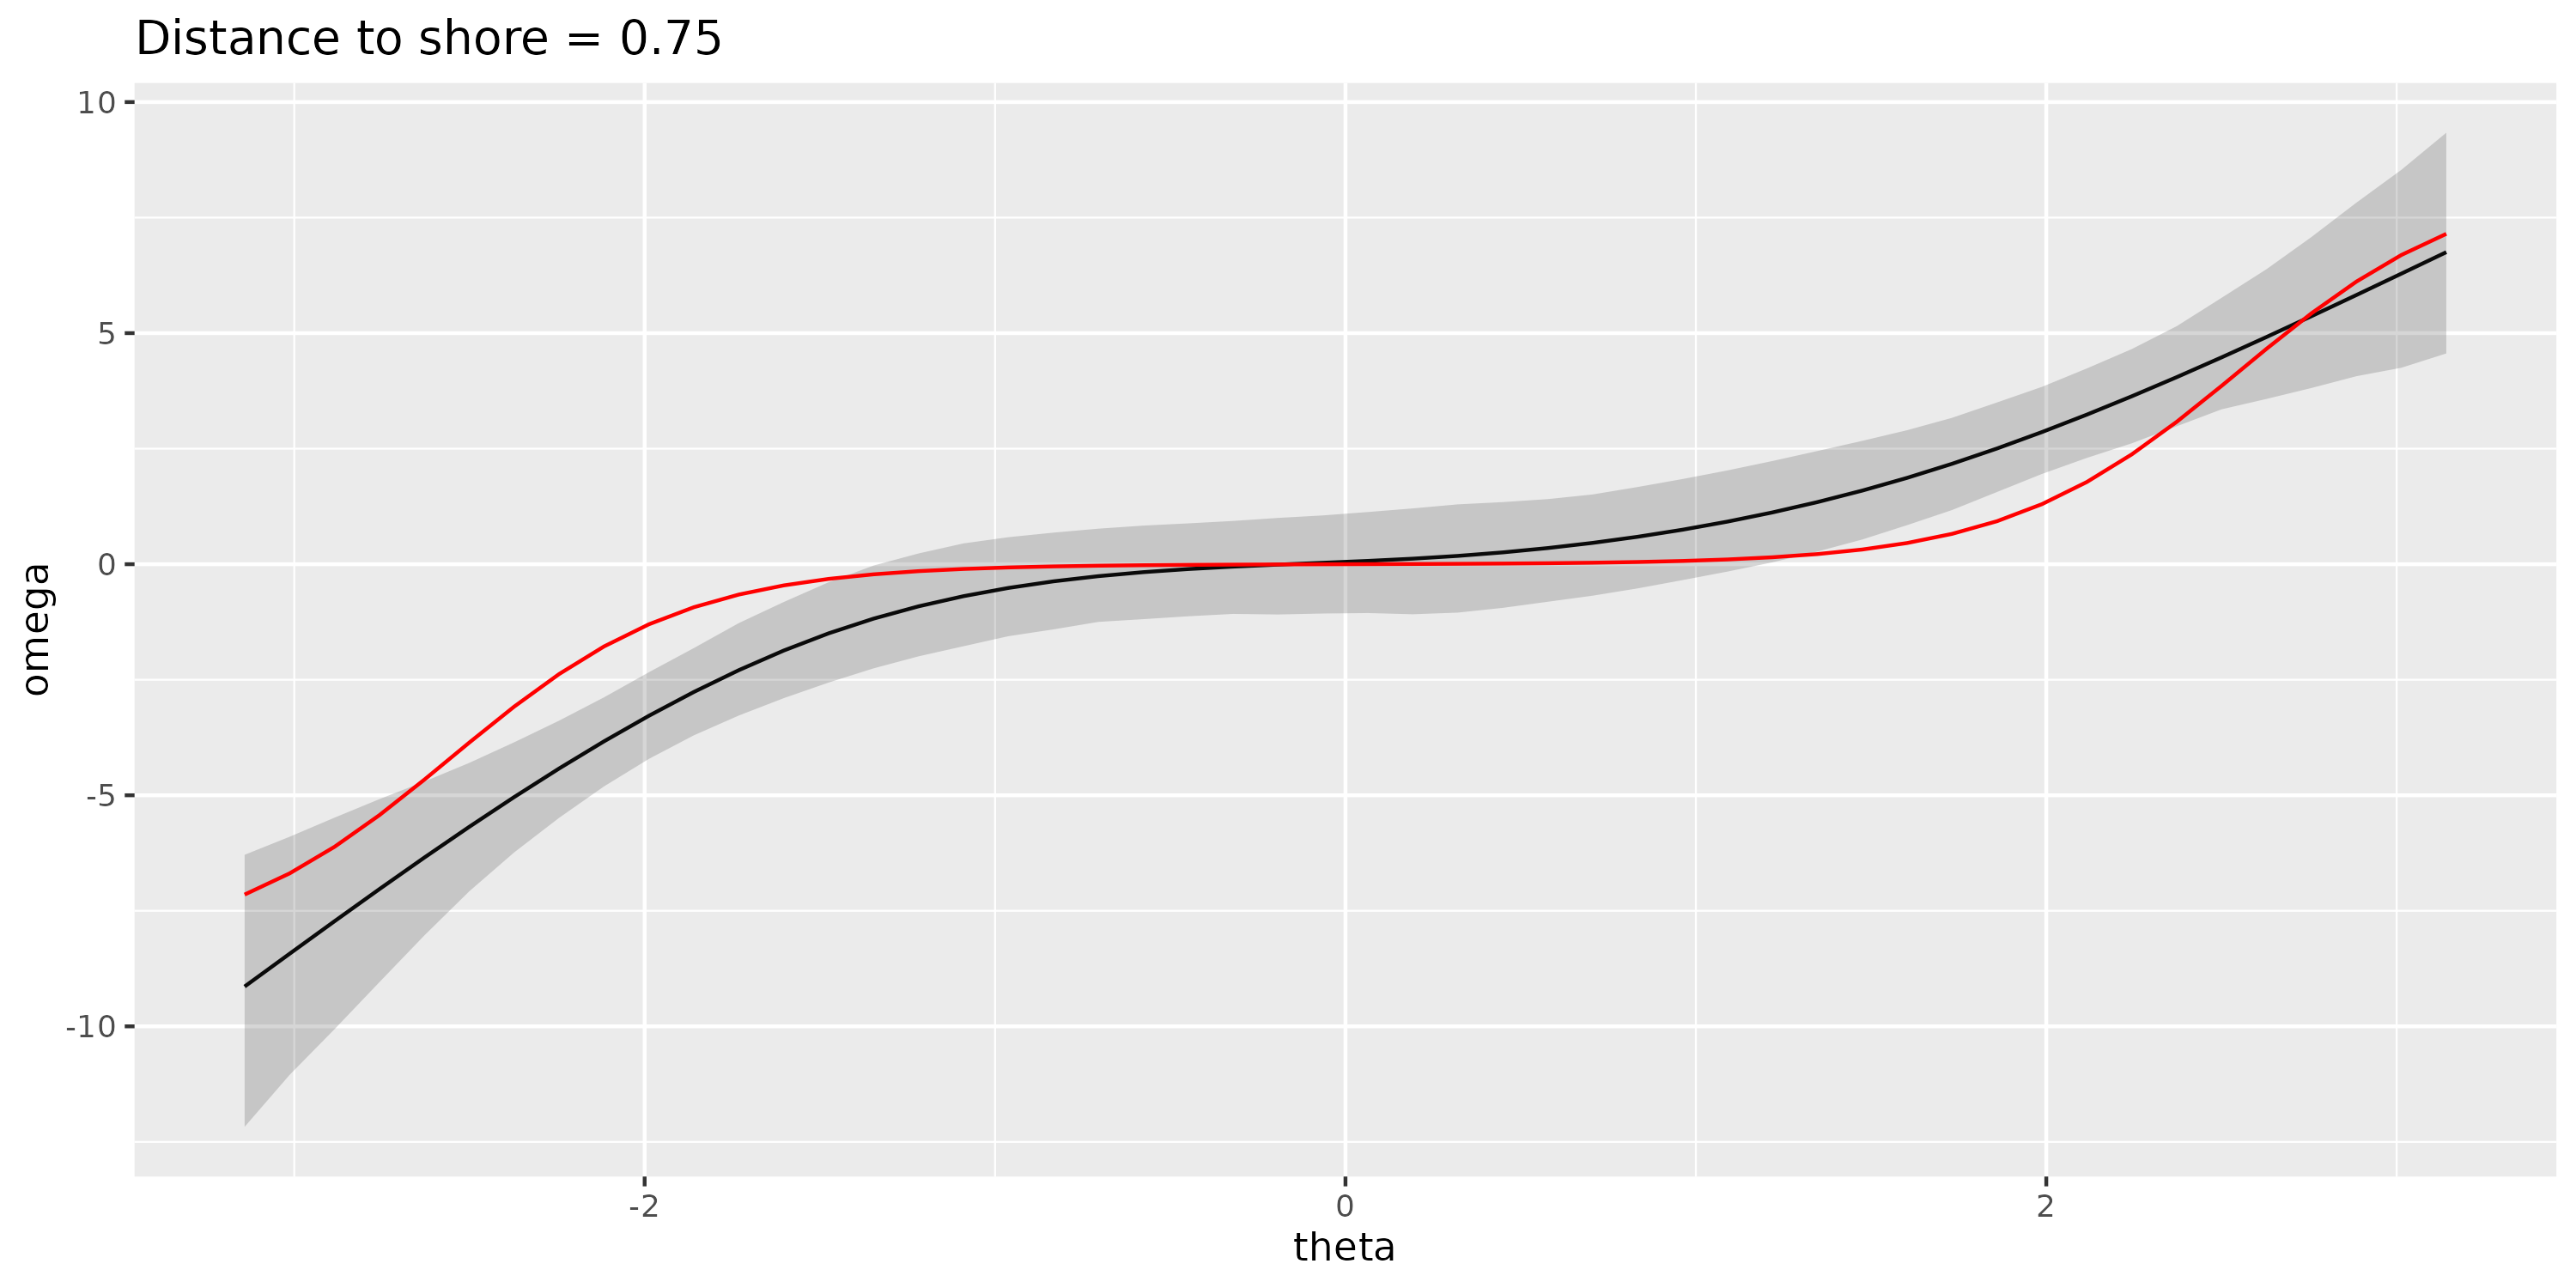
\includegraphics[scale=0.3]{images/simulation study/fe_crcvm_fjords_hf_ne1_omega_theta_q4_ExpShore .png}
		\caption{}
	\end{subfigure}
	\begin{subfigure}{0.48\textwidth}
		\centering
		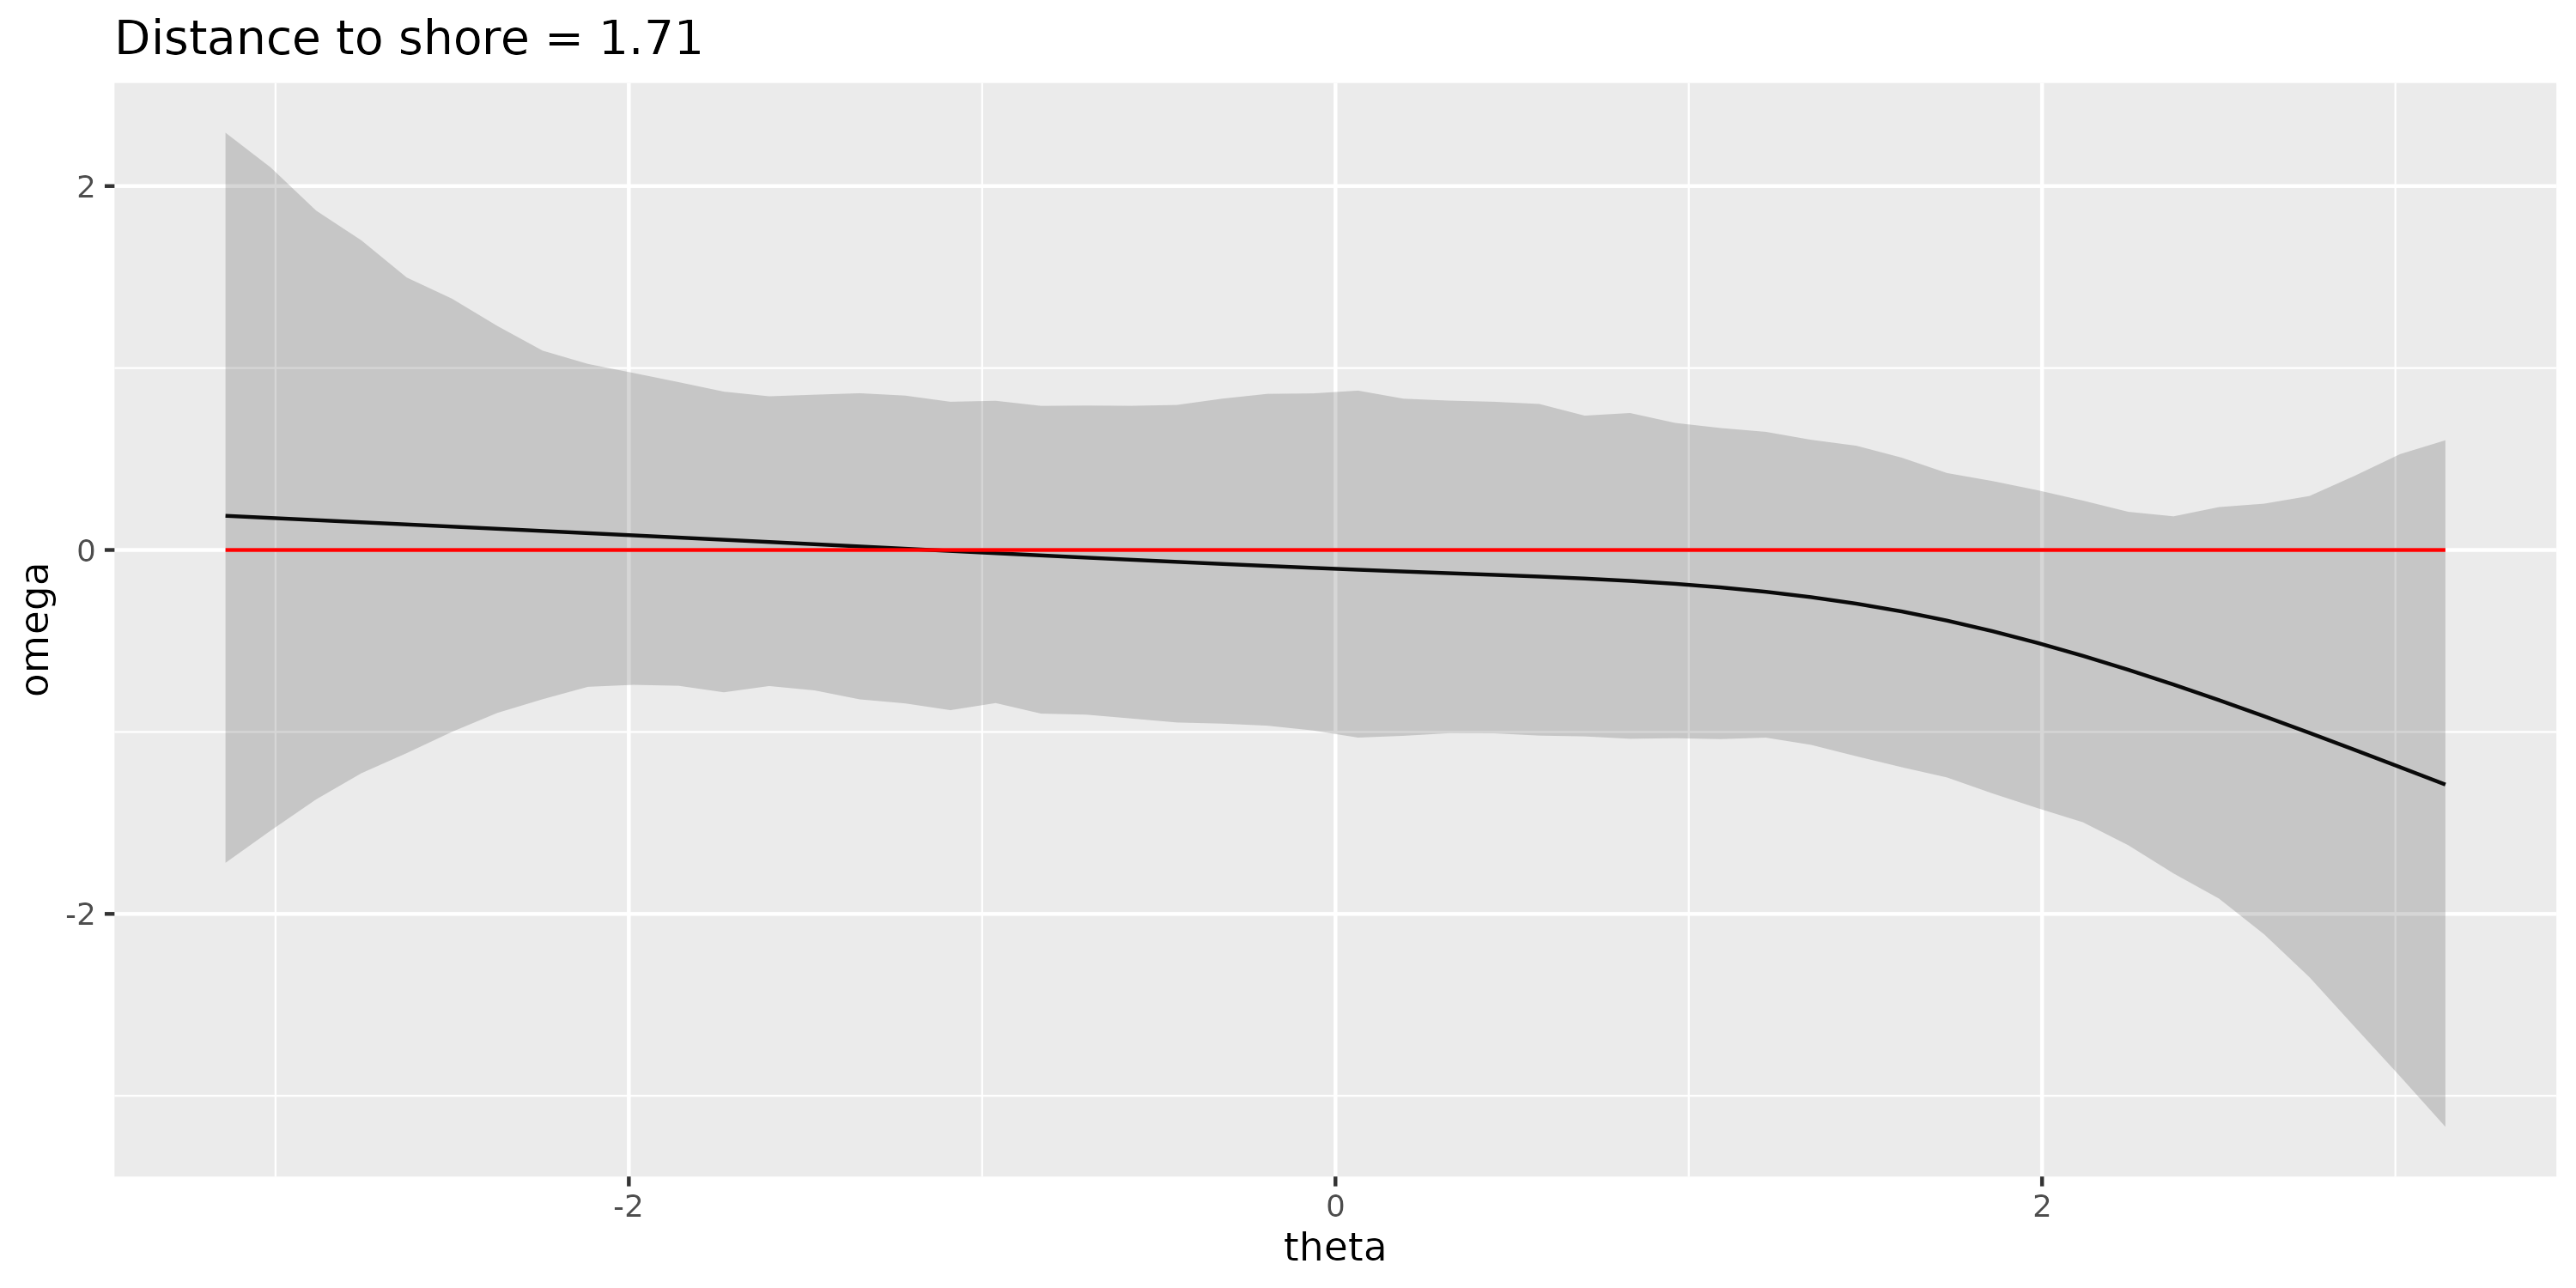
\includegraphics[scale=0.3]{images/simulation study/fe_crcvm_fjords_hf_ne1_omega_theta_q2_ExpShore .png}
		\caption{}
	\end{subfigure}
	\caption{Estimates of the smooth parameter $\omega$ as a function of $\Theta$ only, with distance to shore equal to the $25\%$ and $75\%$ quantiles of observed distances. The red curve represents the true value of $\omega$.}
	\label{fig: marginal_estimates_CRCVM}
\end{figure}



\begin{table}[H]
	\centering
		\begin{tabular}{|c|c|c|c|c|c|c|c|c|c|c|c|c|c|}
		\hline
		&\multicolumn{3}{|c|}{Intercepts} & \multicolumn{8}{|c|}{Spline coefficients} & \multicolumn{2}{|c|}{SD} \\
		\hline
		&$\log(\tau_0)$ & $\log(\nu_0)$ & $\omega_0$ & $\omega_1$ & $\omega_2$ & $\omega_3$ & $\omega_4$  & $\omega_5$ & $\omega_6$ & $\omega_7$ & $\omega_8$ & $\sigma_{\tau}$ & $\sigma_{\nu}$ \\
		\hline 
		 True values & $0$ & $1.39$ & $0.01$ & $6.47$ & $-2.07$ & $4.62$ & $15.44$ & $4.62$ & $21.10$ & $2.91$ & $4.86$ & $0.2$ & $0.1$ \\
		\hline
			\multicolumn{14}{|c|}{Estimates for $d(X_0,\mathcal{D}) > 4$ km} \\
			\hline
	\multirow{2}{4em}{$N=6$} & & & & & & & & & & & & &\\
	& & & & & & & & & & & & & \\
	\hline
	\multirow{2}{4em}{$N=12$} & -0.03 & 1.38 & -0.02
	&5.82&-1.60 & 3.84 & 14.59 &4.06 & 19.77 & 3.04 & 4.20 & 0.09& 
	0.09\\
	& 0.09 & 0.04 & 0.17 & 0.64 &0.83 &0.81 & 1.08 & 1.83 & 1.02 &0.65 &0.77 &
	0.08 & 0.03  \\
	\hline	
\end{tabular}
\end{table}



\section{Application to narwhals behavioral response}


In this section, we apply our diffusion models to analyse a behavioral response of the narwhals to ship and seismic airguns exposure.
A baseline model is fitted on the narwhals's track before exposure. It is supposed to capture the characteristics of the movement under normal conditions. Deviation from the baseline is then assessed by fitting a model with covariate $E^{ship}$ on the tracks during exposure.


\subsection{Baseline estimations}

The persistence is estimated to $\hat{\tau}_{0}=1.3 $ h.
In comparison, harbour seal in Alaska were proved to exhibit slightly more persistent motion $\hat{\tau}=1.51$ h with $95\%$ CI ; $1.30 -1.75$  \cite{johnson_continuoustime_2008} while bowhead whales in Greenland showed much less persistence $\hat{\tau}=0.17$ h with $95\%$ CI ; $0.14 -0.20$  \cite{gurarie_correlated_2017}.
The intercept value for $\nu$ is estimated to be $\hat{\nu}_{0}=4.19$ km/h with $95\%$ CI $3.79-4.63$.
\begin{table}[H]
	\centering
	\begin{tabular}{|c|c|c|}
		\hline
		Coefficient   & Estimate  & $95\%$ CI \\
		\hline
		$\log(\tau_0)$   & 0.3    &  \\
		$\log(\nu_0)$  & 1.48  &  \\
		$\omega_0$     & -0.13     &  \\
		$\sigma_{\tau,pre}$   & 0.1   &   \\
		$\sigma_{\nu,pre}$    & 0.1   &  \\
		\hline
	\end{tabular}
	\caption{Intercepts baseline estimations}
	\label{table: baseline estilations}
\end{table}

Figure \ref{fig:febaseline3omegaanglenormalq0} shows the estimated smooth $\omega$ as a function of $\Theta$ for different values of the distance to shore. As distance increases, the magnitude of the angular velocity decreases. 
% PUT ON THE SAME PLOT WITH DIFFERENT COLOR FOR EACH CURVE
\begin{figure}[H]
	\begin{subfigure}{0.33\textwidth}
		\centering
		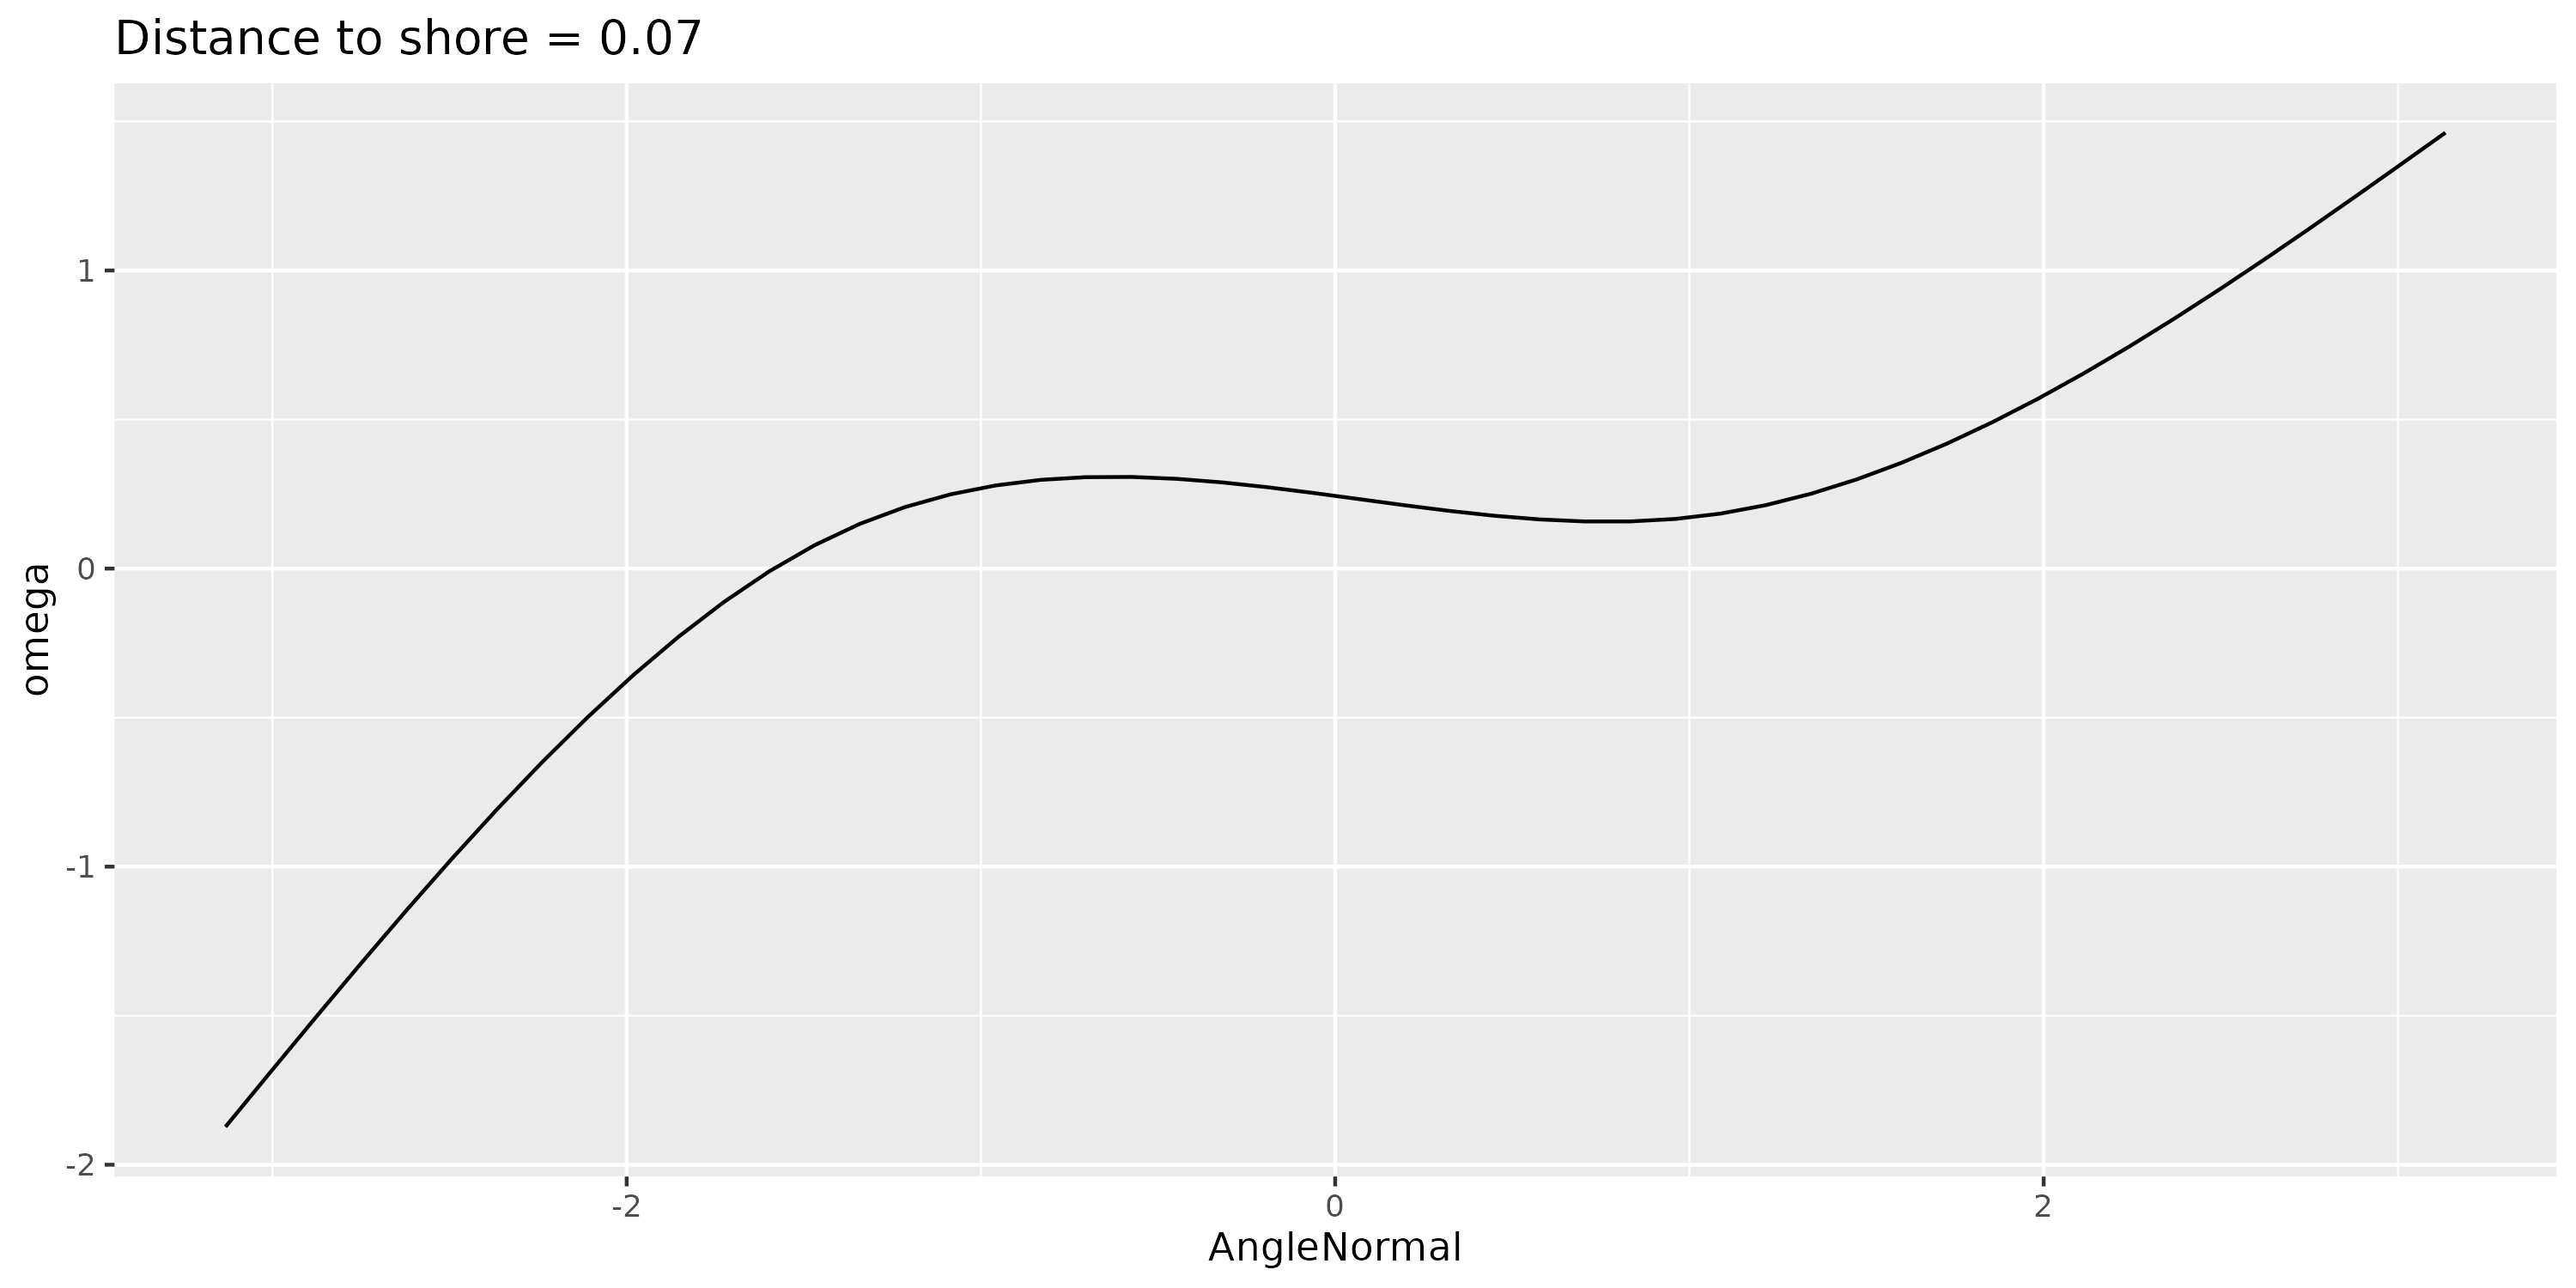
\includegraphics[width=0.95\linewidth]{"images/application/baseline/fe_baseline3_omega_AngleNormal_q0.95_ExpShore .png"}
	\end{subfigure}
	\begin{subfigure}{0.33\textwidth}
		\centering
		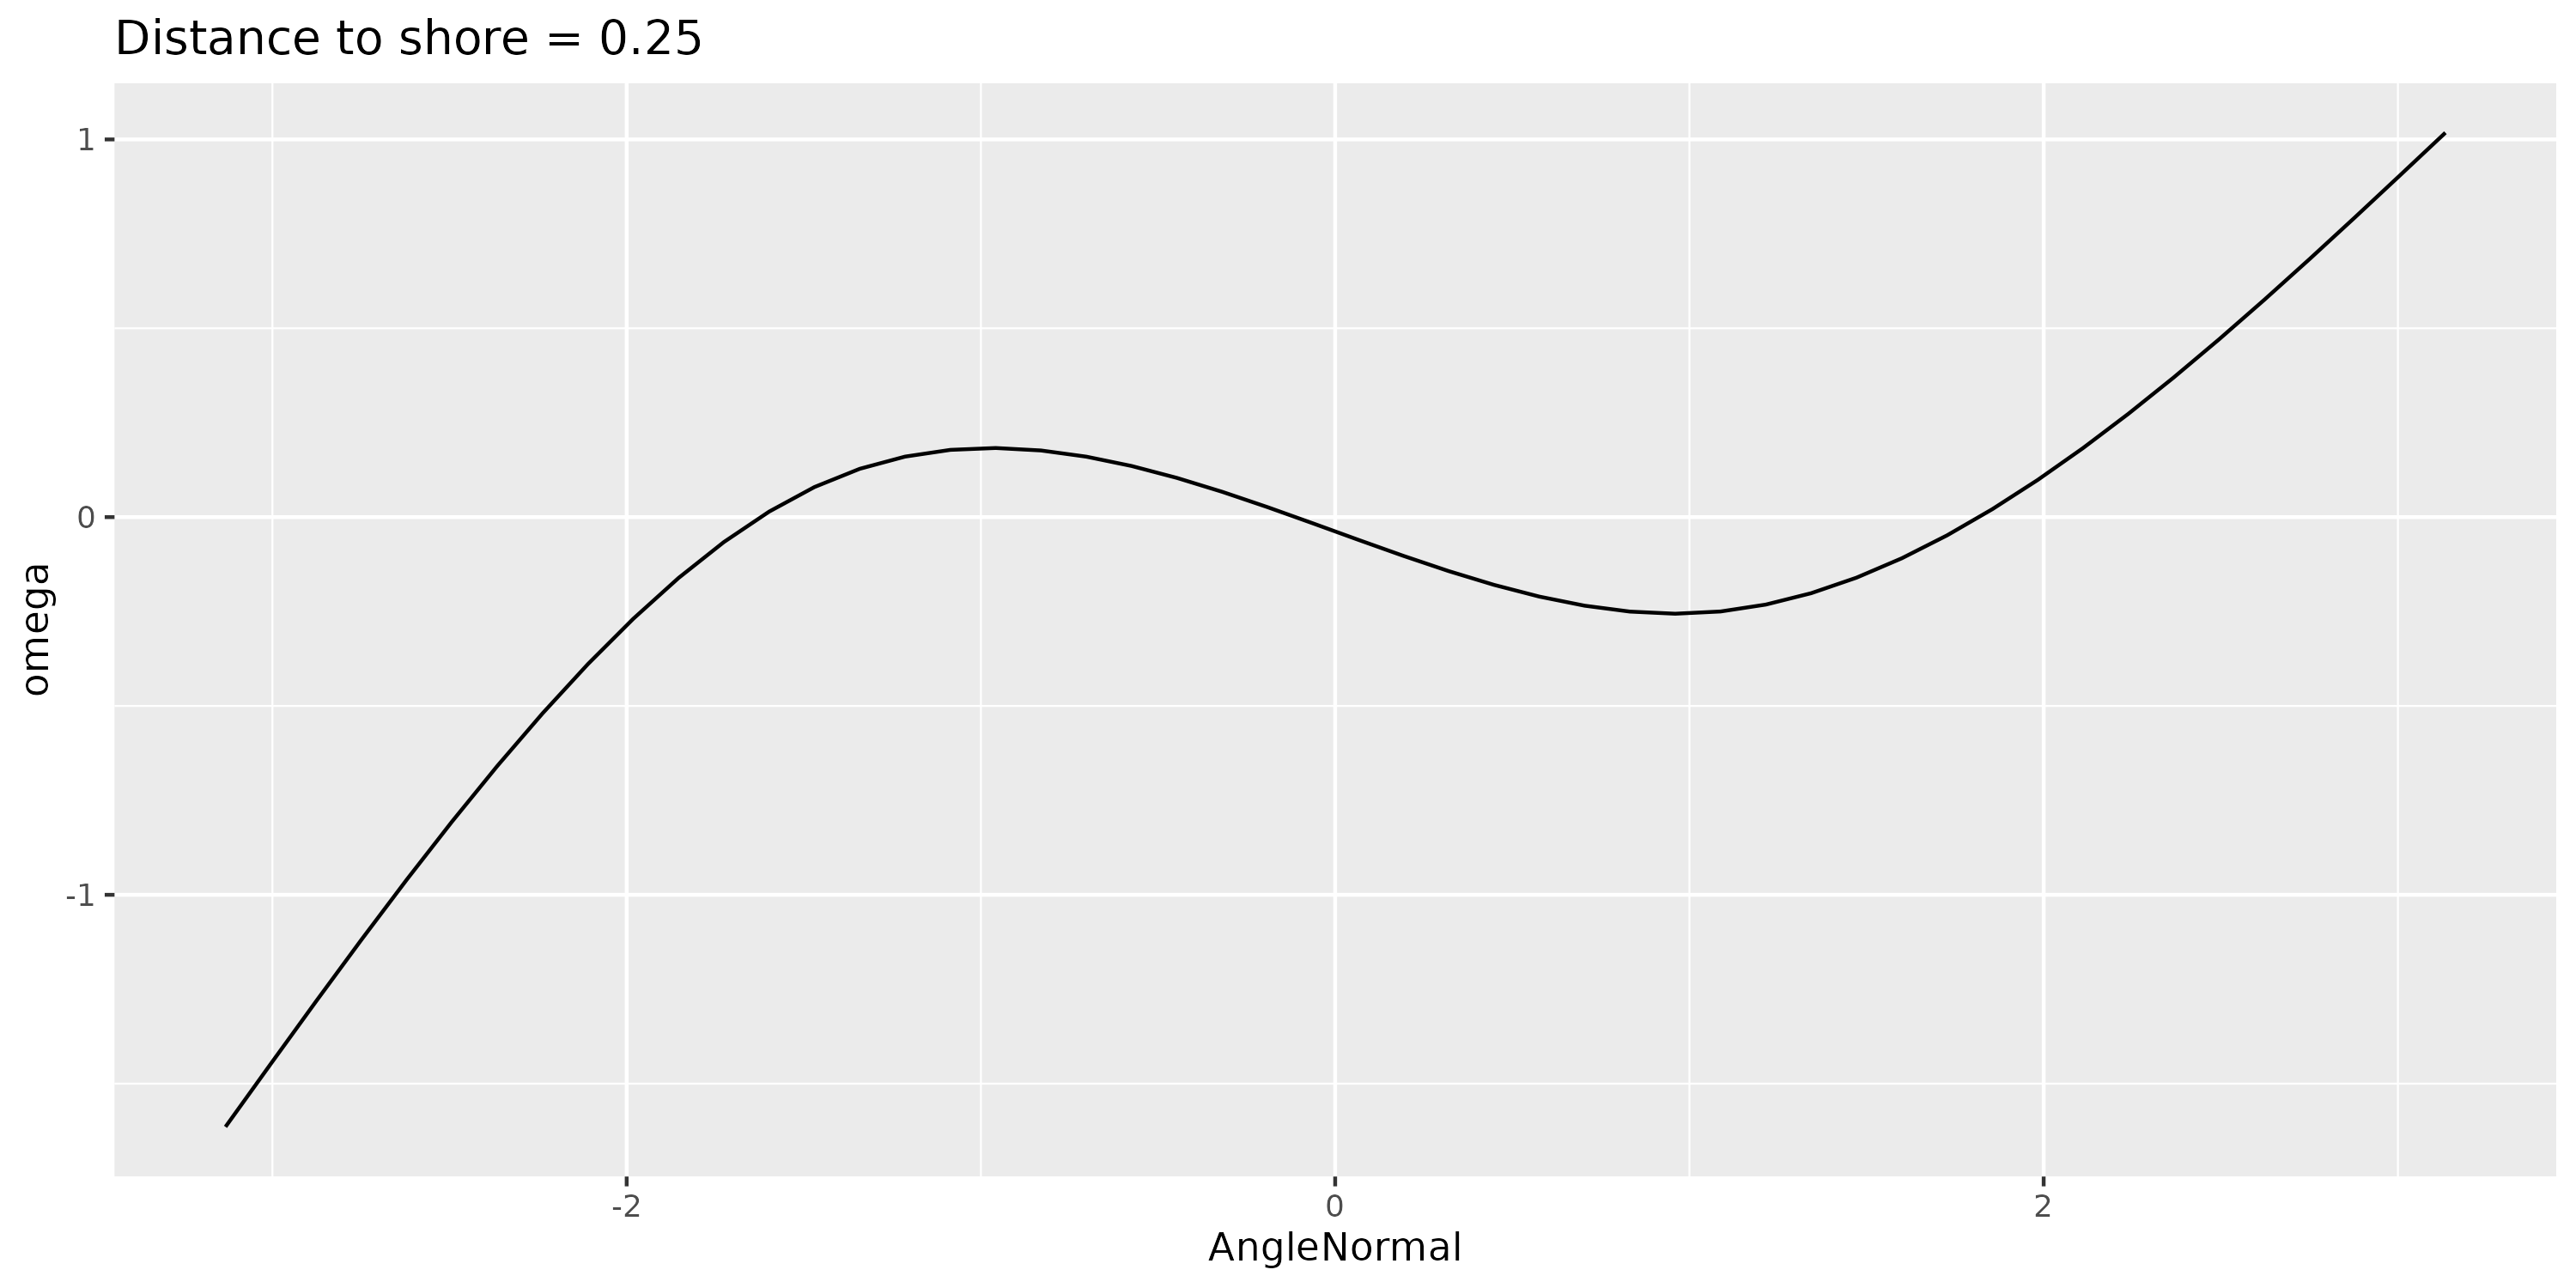
\includegraphics[width=0.95\linewidth]{"images/application/baseline/fe_baseline3_omega_AngleNormal_q0.75_ExpShore .png"}
	\end{subfigure}
	\begin{subfigure}{0.33\textwidth}
		\centering
		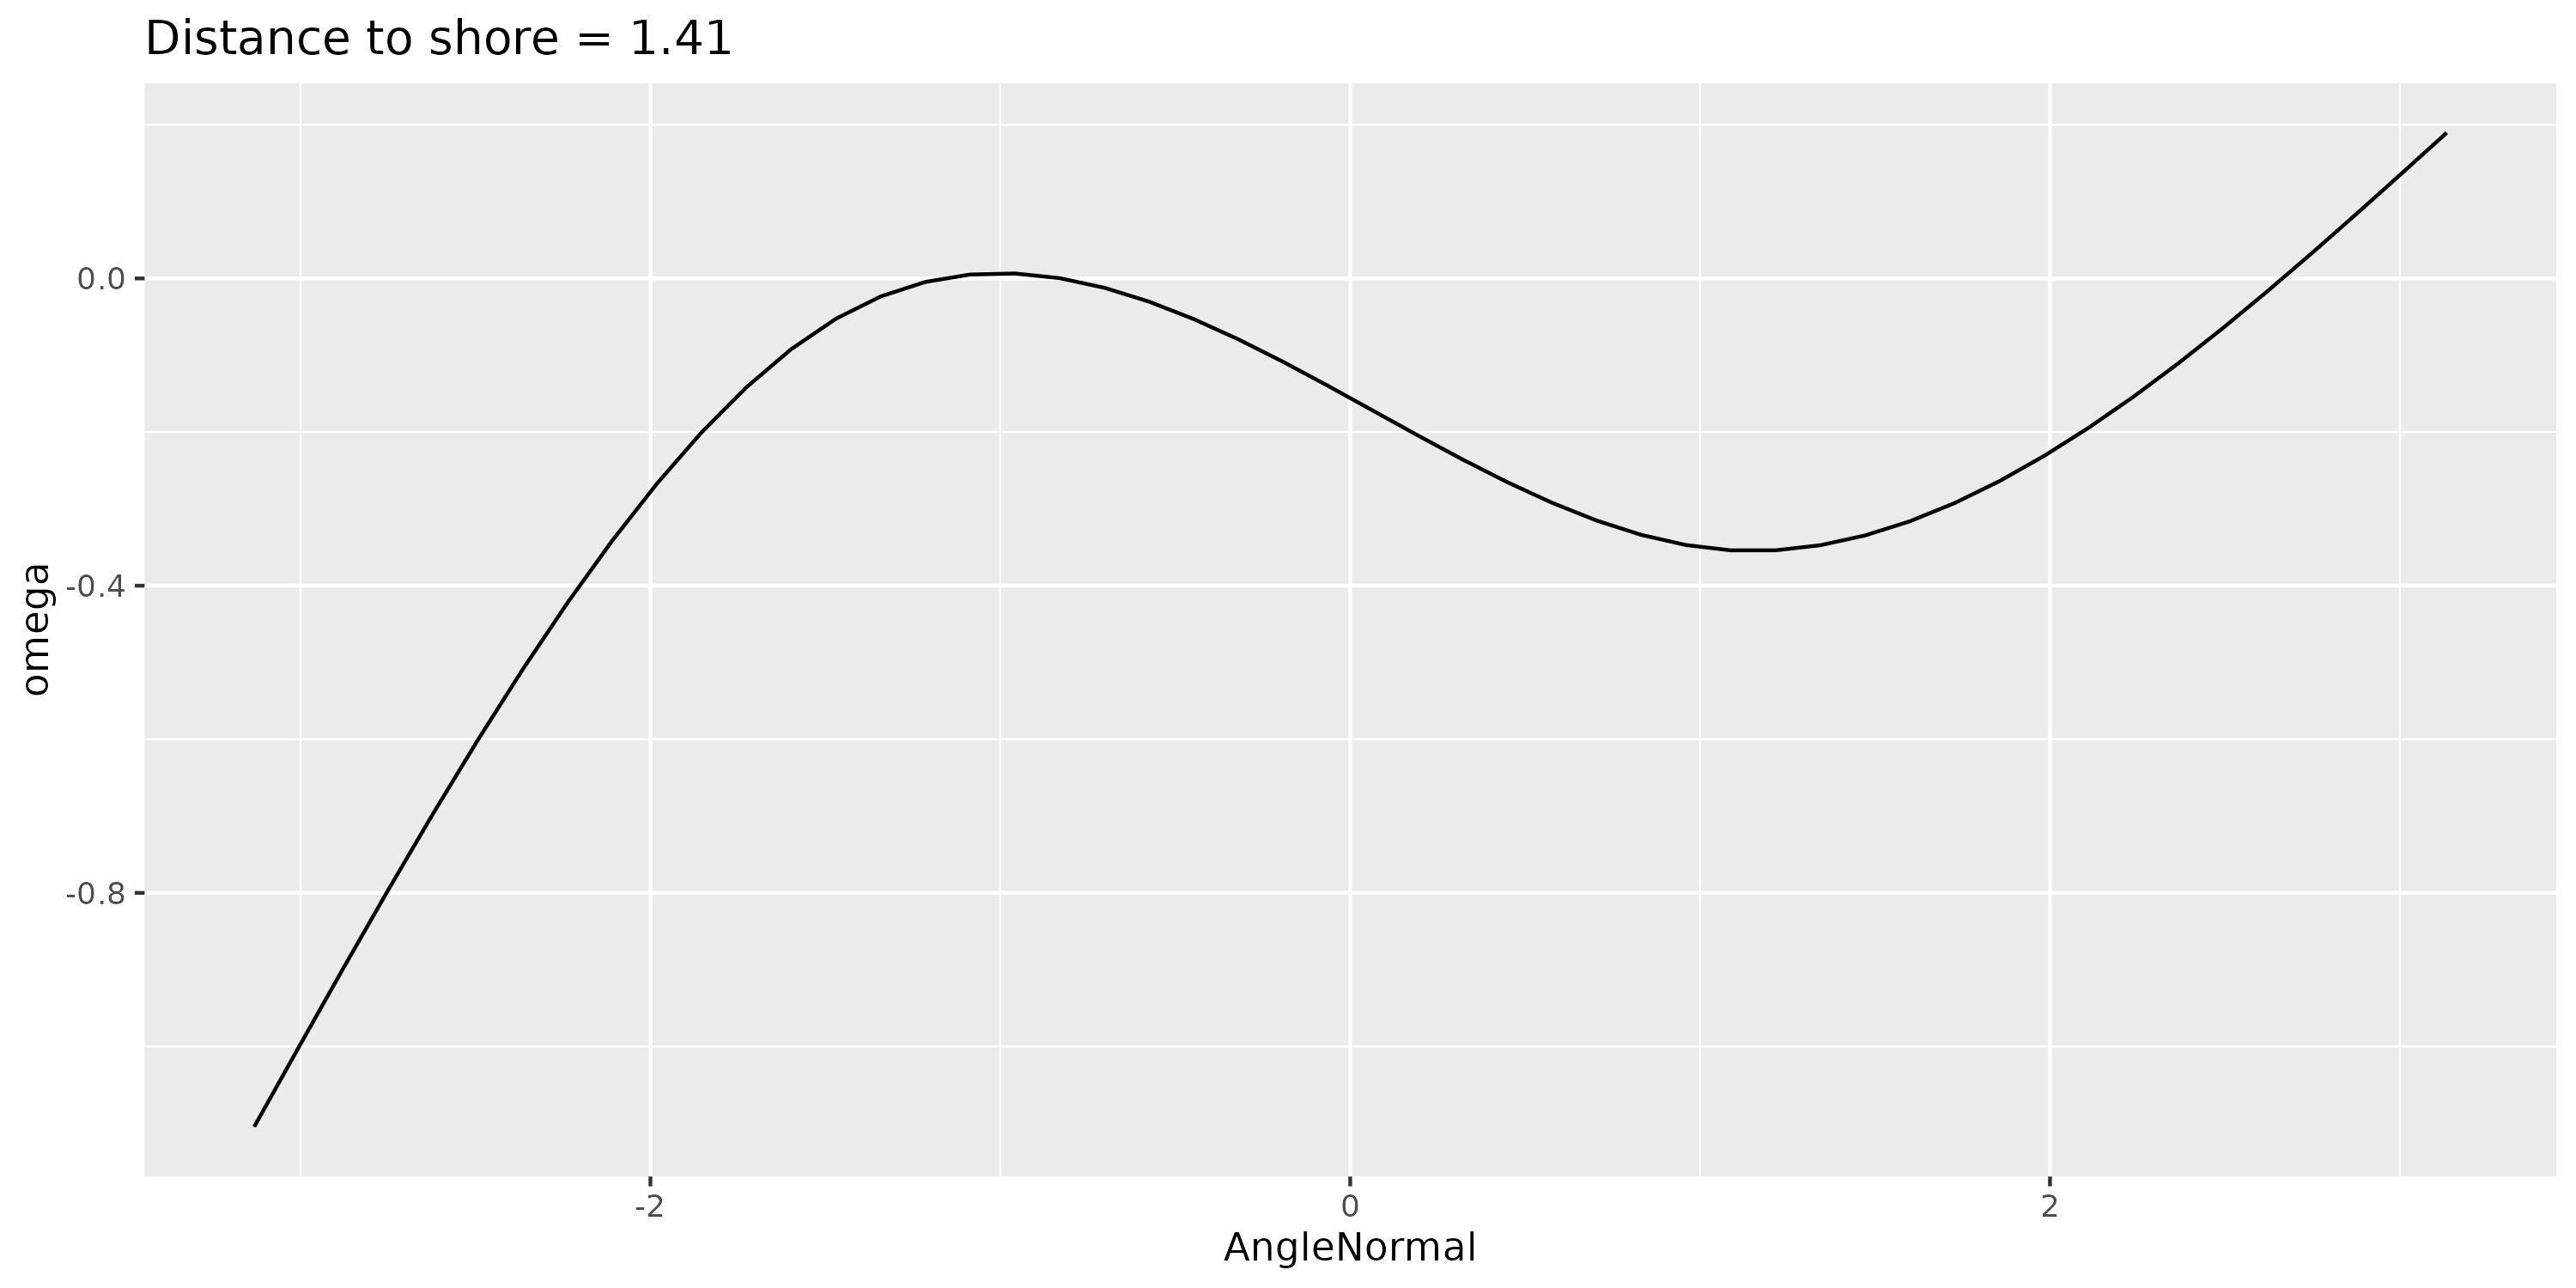
\includegraphics[width=0.95\linewidth]{"images/application/baseline/fe_baseline3_omega_AngleNormal_q0.25_ExpShore .png"}
	\end{subfigure}
	\caption{}

	\label{fig:febaseline3omegaanglenormalq0}
\end{figure}






\subsection{Response estimations}

\begin{comment}
\begin{figure}[H]
	\centering
	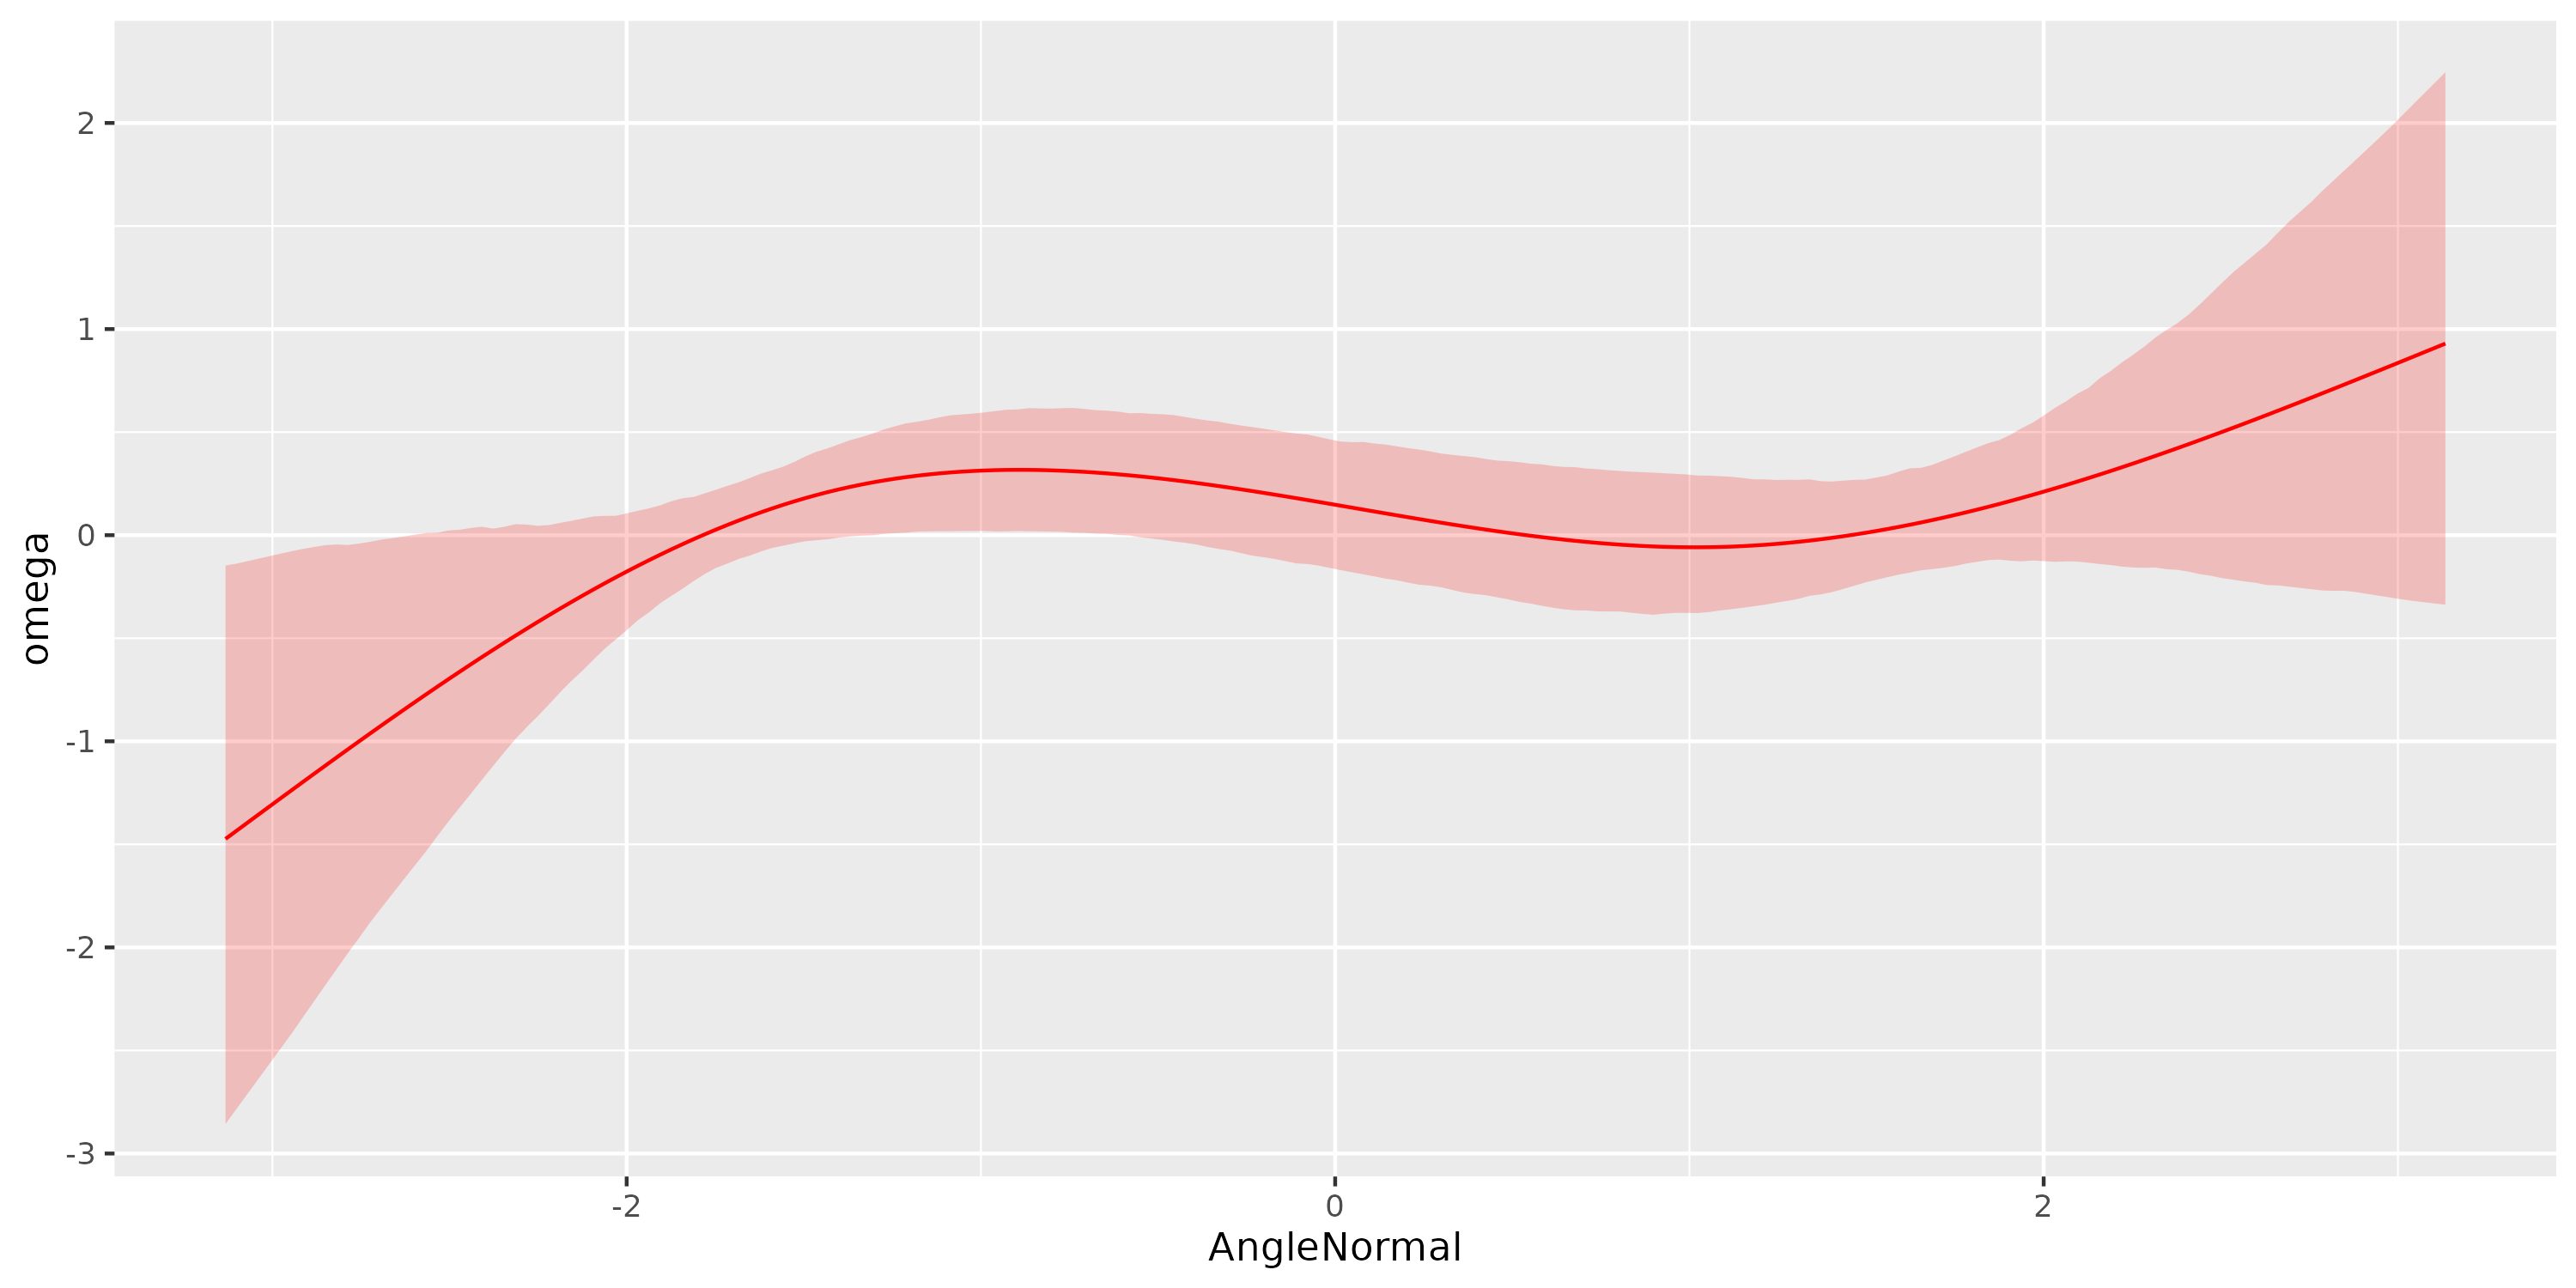
\includegraphics[width=0.7\linewidth]{images/application/fe_baseline1_omega_AngleNormal}
	\caption{}
	\label{fig:febaseline1omegaanglenormal}
\end{figure}
\begin{figure}[H]
	\centering
	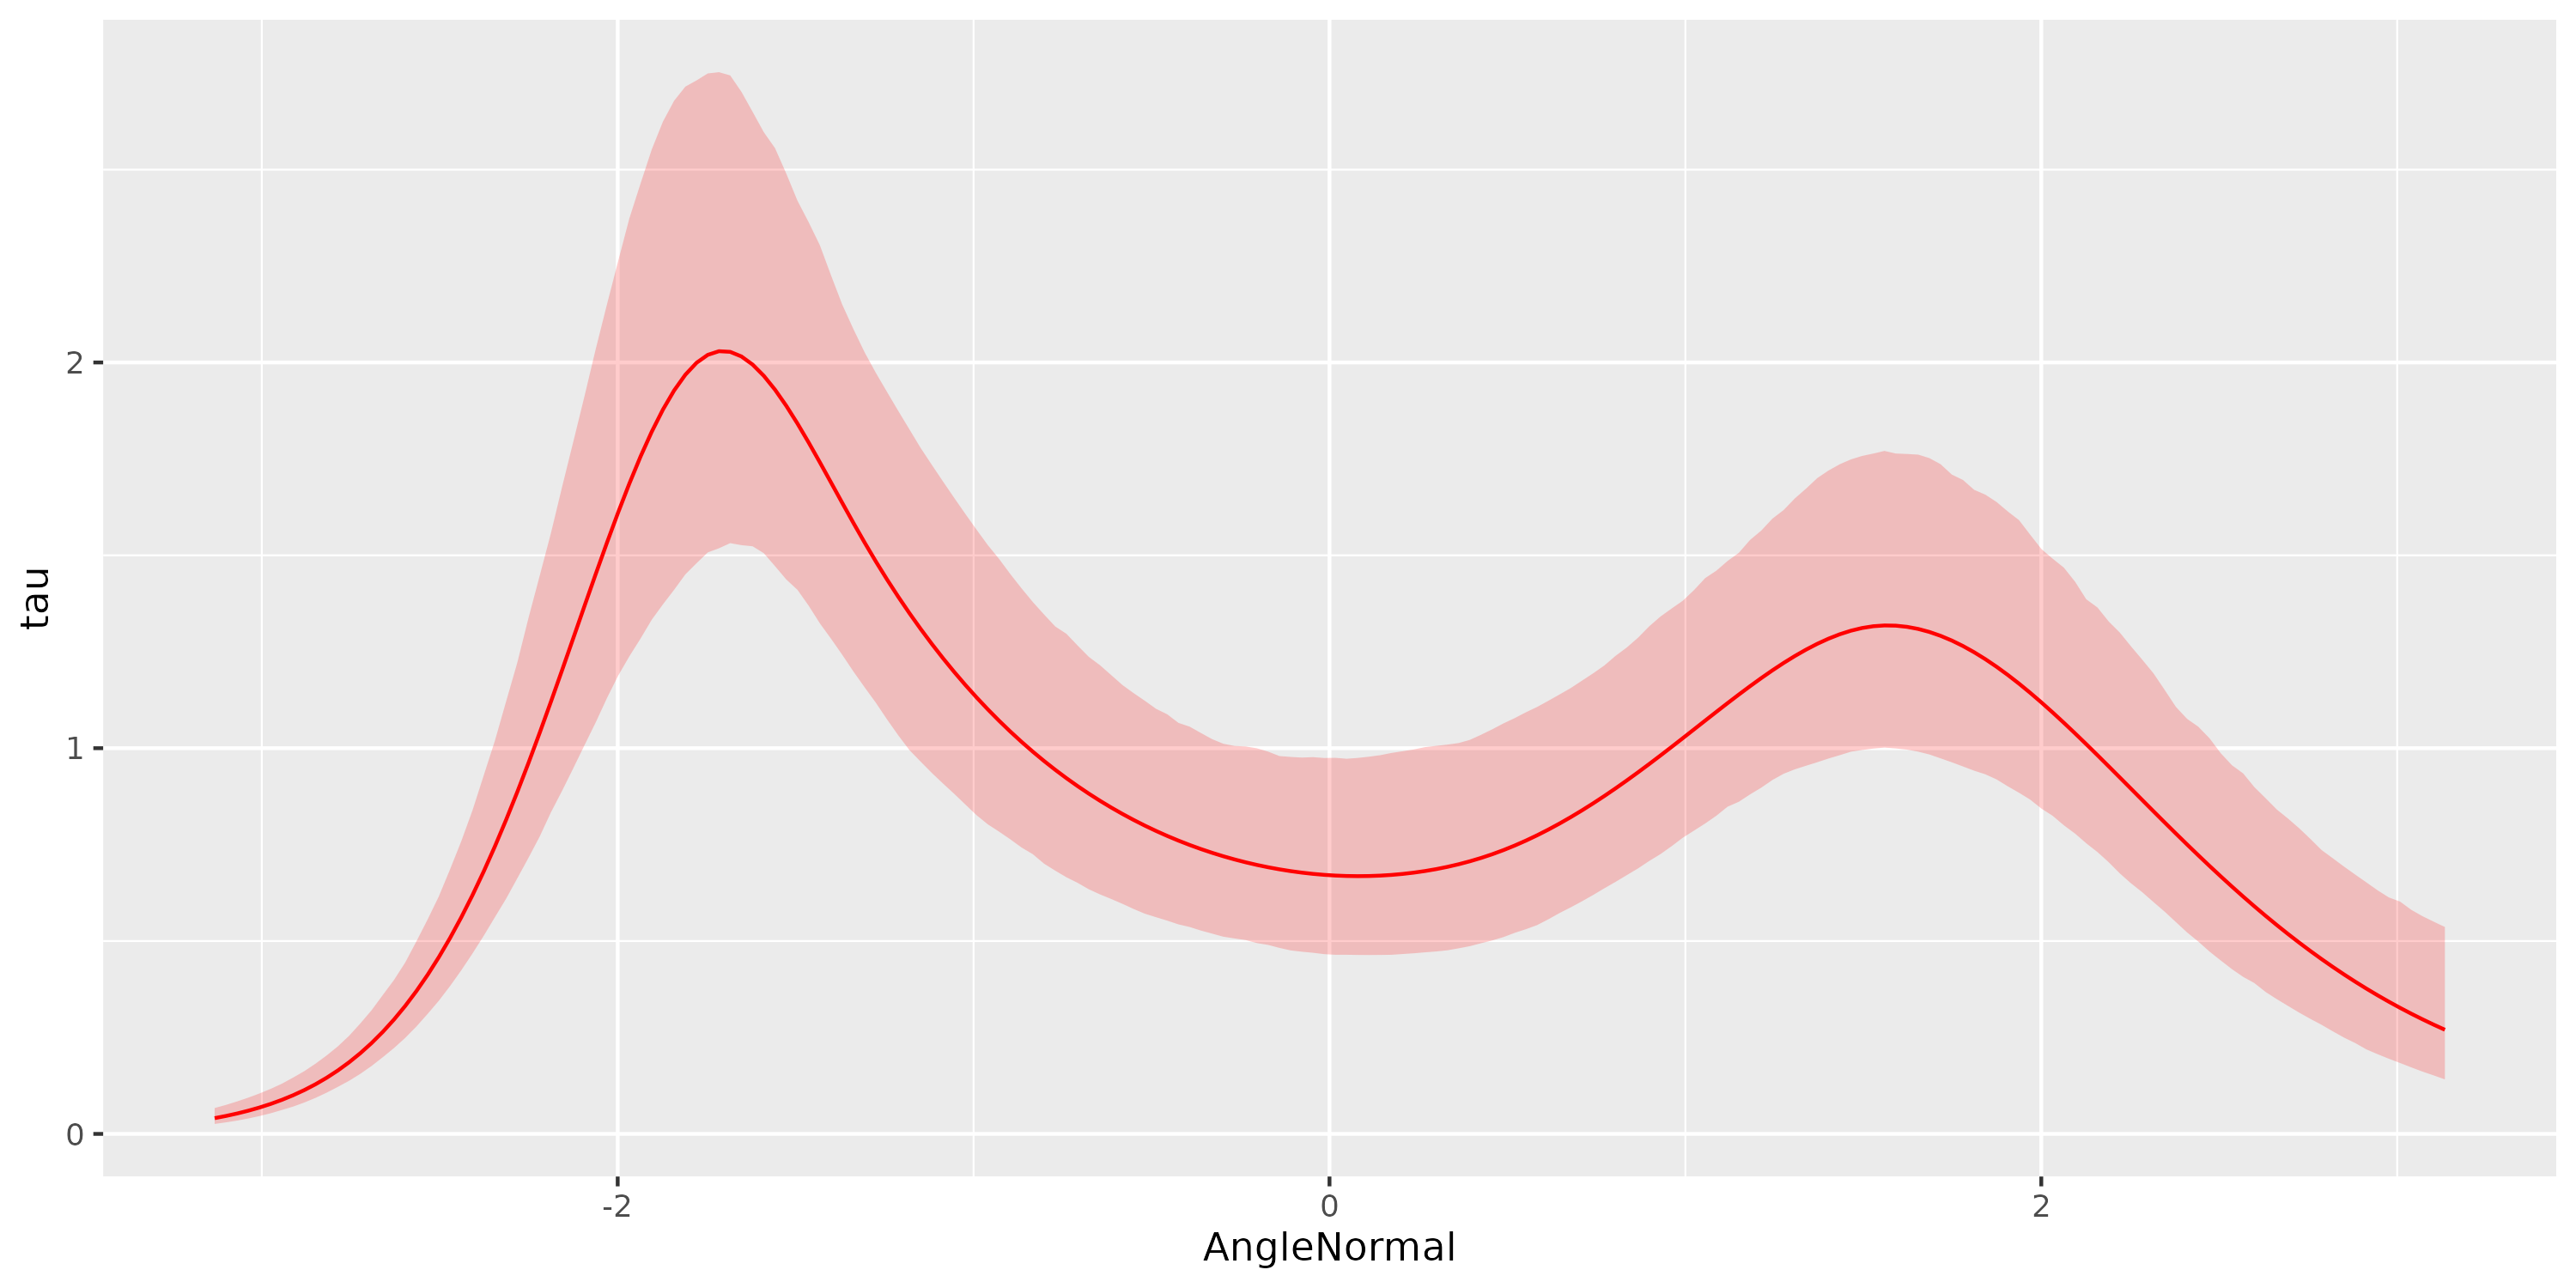
\includegraphics[width=0.7\linewidth]{images/application/fe_baseline1_tau_AngleNormal}
	\caption{}
	\label{fig:febaseline1tauanglenormal}
\end{figure}


\subsubsection{Estimation without constraints}

First, a simple CVM was used to assess any behavioural response of the narwhals to the ship exposure.

\paragraph{Baseline estimations}
Due to the low variability of the estimates of $\tau$ for each individual, it was chosen to only estimate one intercept value for this parameter. It was estimated to $\hat{\tau}_{pre}=0.90 $ km/h with $95 \%$ of its values comprised between $0.85$ and $1.1$ h.
In comparison, harbour seal in Alaska were proved to exhibit slightly more persistent motion $\hat{\tau}=1.51$ h with $95\%$ CI ; $1.30 -1.75$  \cite{johnson_continuous_2008} while bowhead whales in Greenland showed much less persistence $\hat{\tau}=0.17$ h with $95\%$ CI ; $0.14 -0.20$  \cite{gurarie_correlated_2017}.
The intercept value for $\nu$ was estimated to be $\hat{\nu}_{pre}=4.19$ km/h with $95\%$ CI $3.79-4.63$.
The estimates for the long term velocity $\mu$ show that all the narwhals have a tendency to move toward the south ($\mu_2<0$) with more individual variability for the east-west direction $\mu_1$. However, confidence intervals are large and  forcing $\mu$ to $(0,0)$ is also a reasonable choice.

\begin{figure}[H]
    \centering
  
    \begin{subfigure}{0.49\textwidth}
    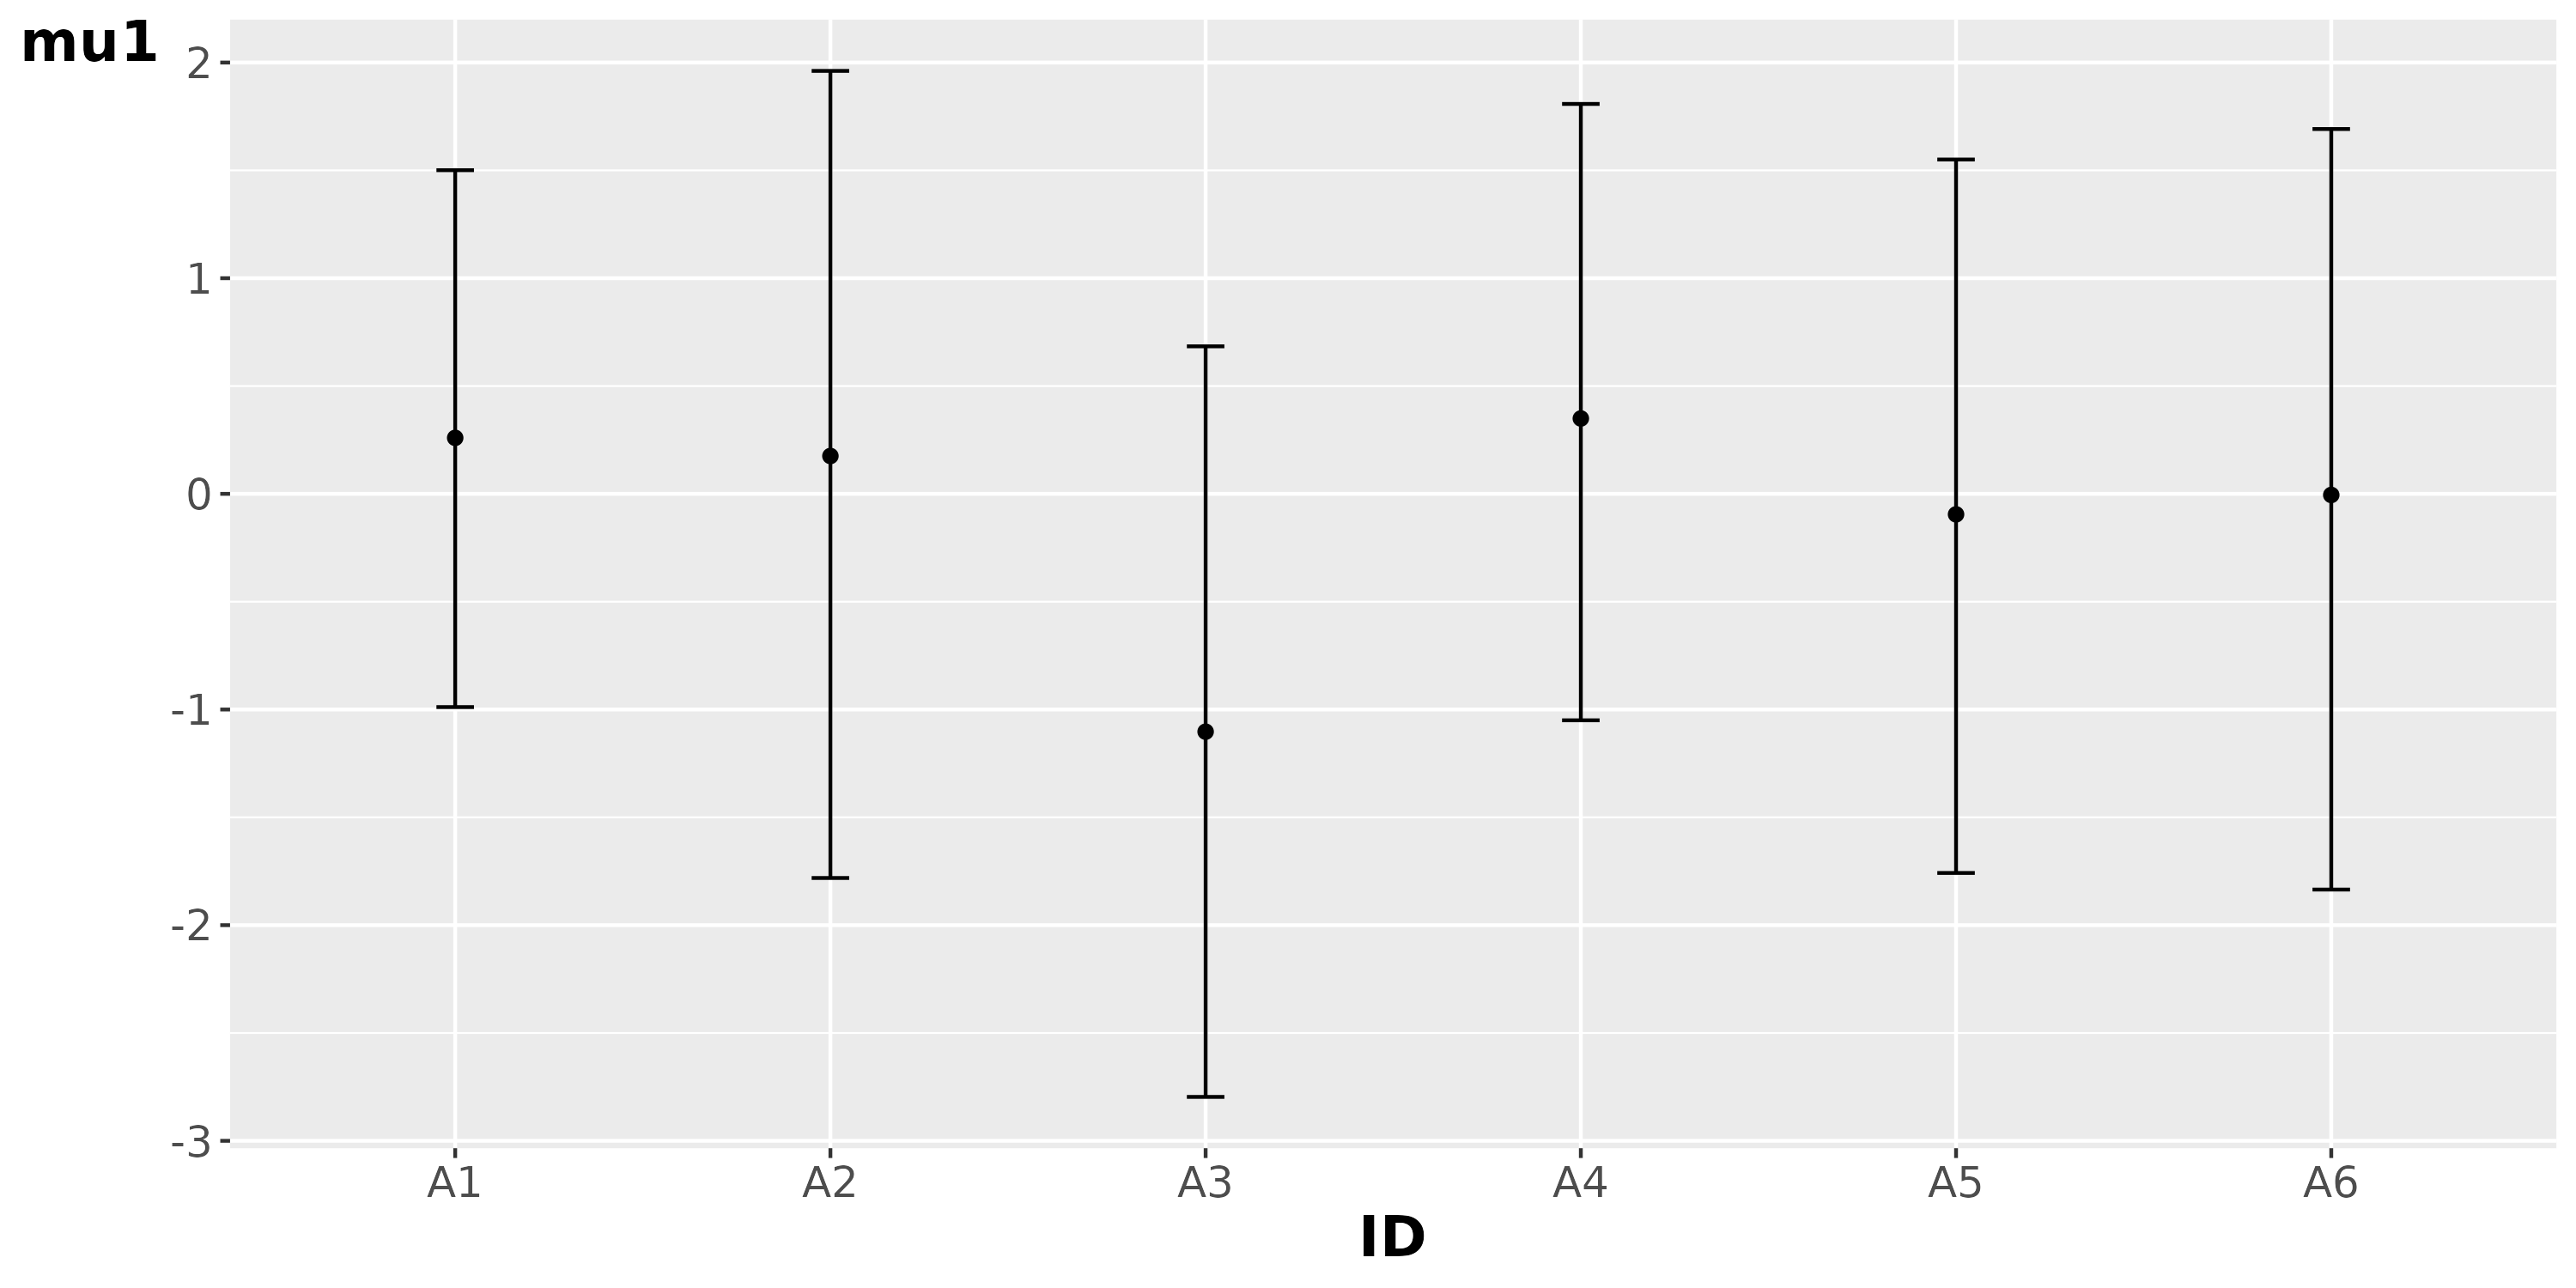
\includegraphics[scale=0.3]{images/unconstrained_models/baseline/re_baseline2_mu1.png}
    \caption{Estimated $\mu_1$ (km/h) for the baseline model}
    \label{fig: re_baseline1_mu1}
    \end{subfigure}
     \begin{subfigure}{0.49\textwidth}
    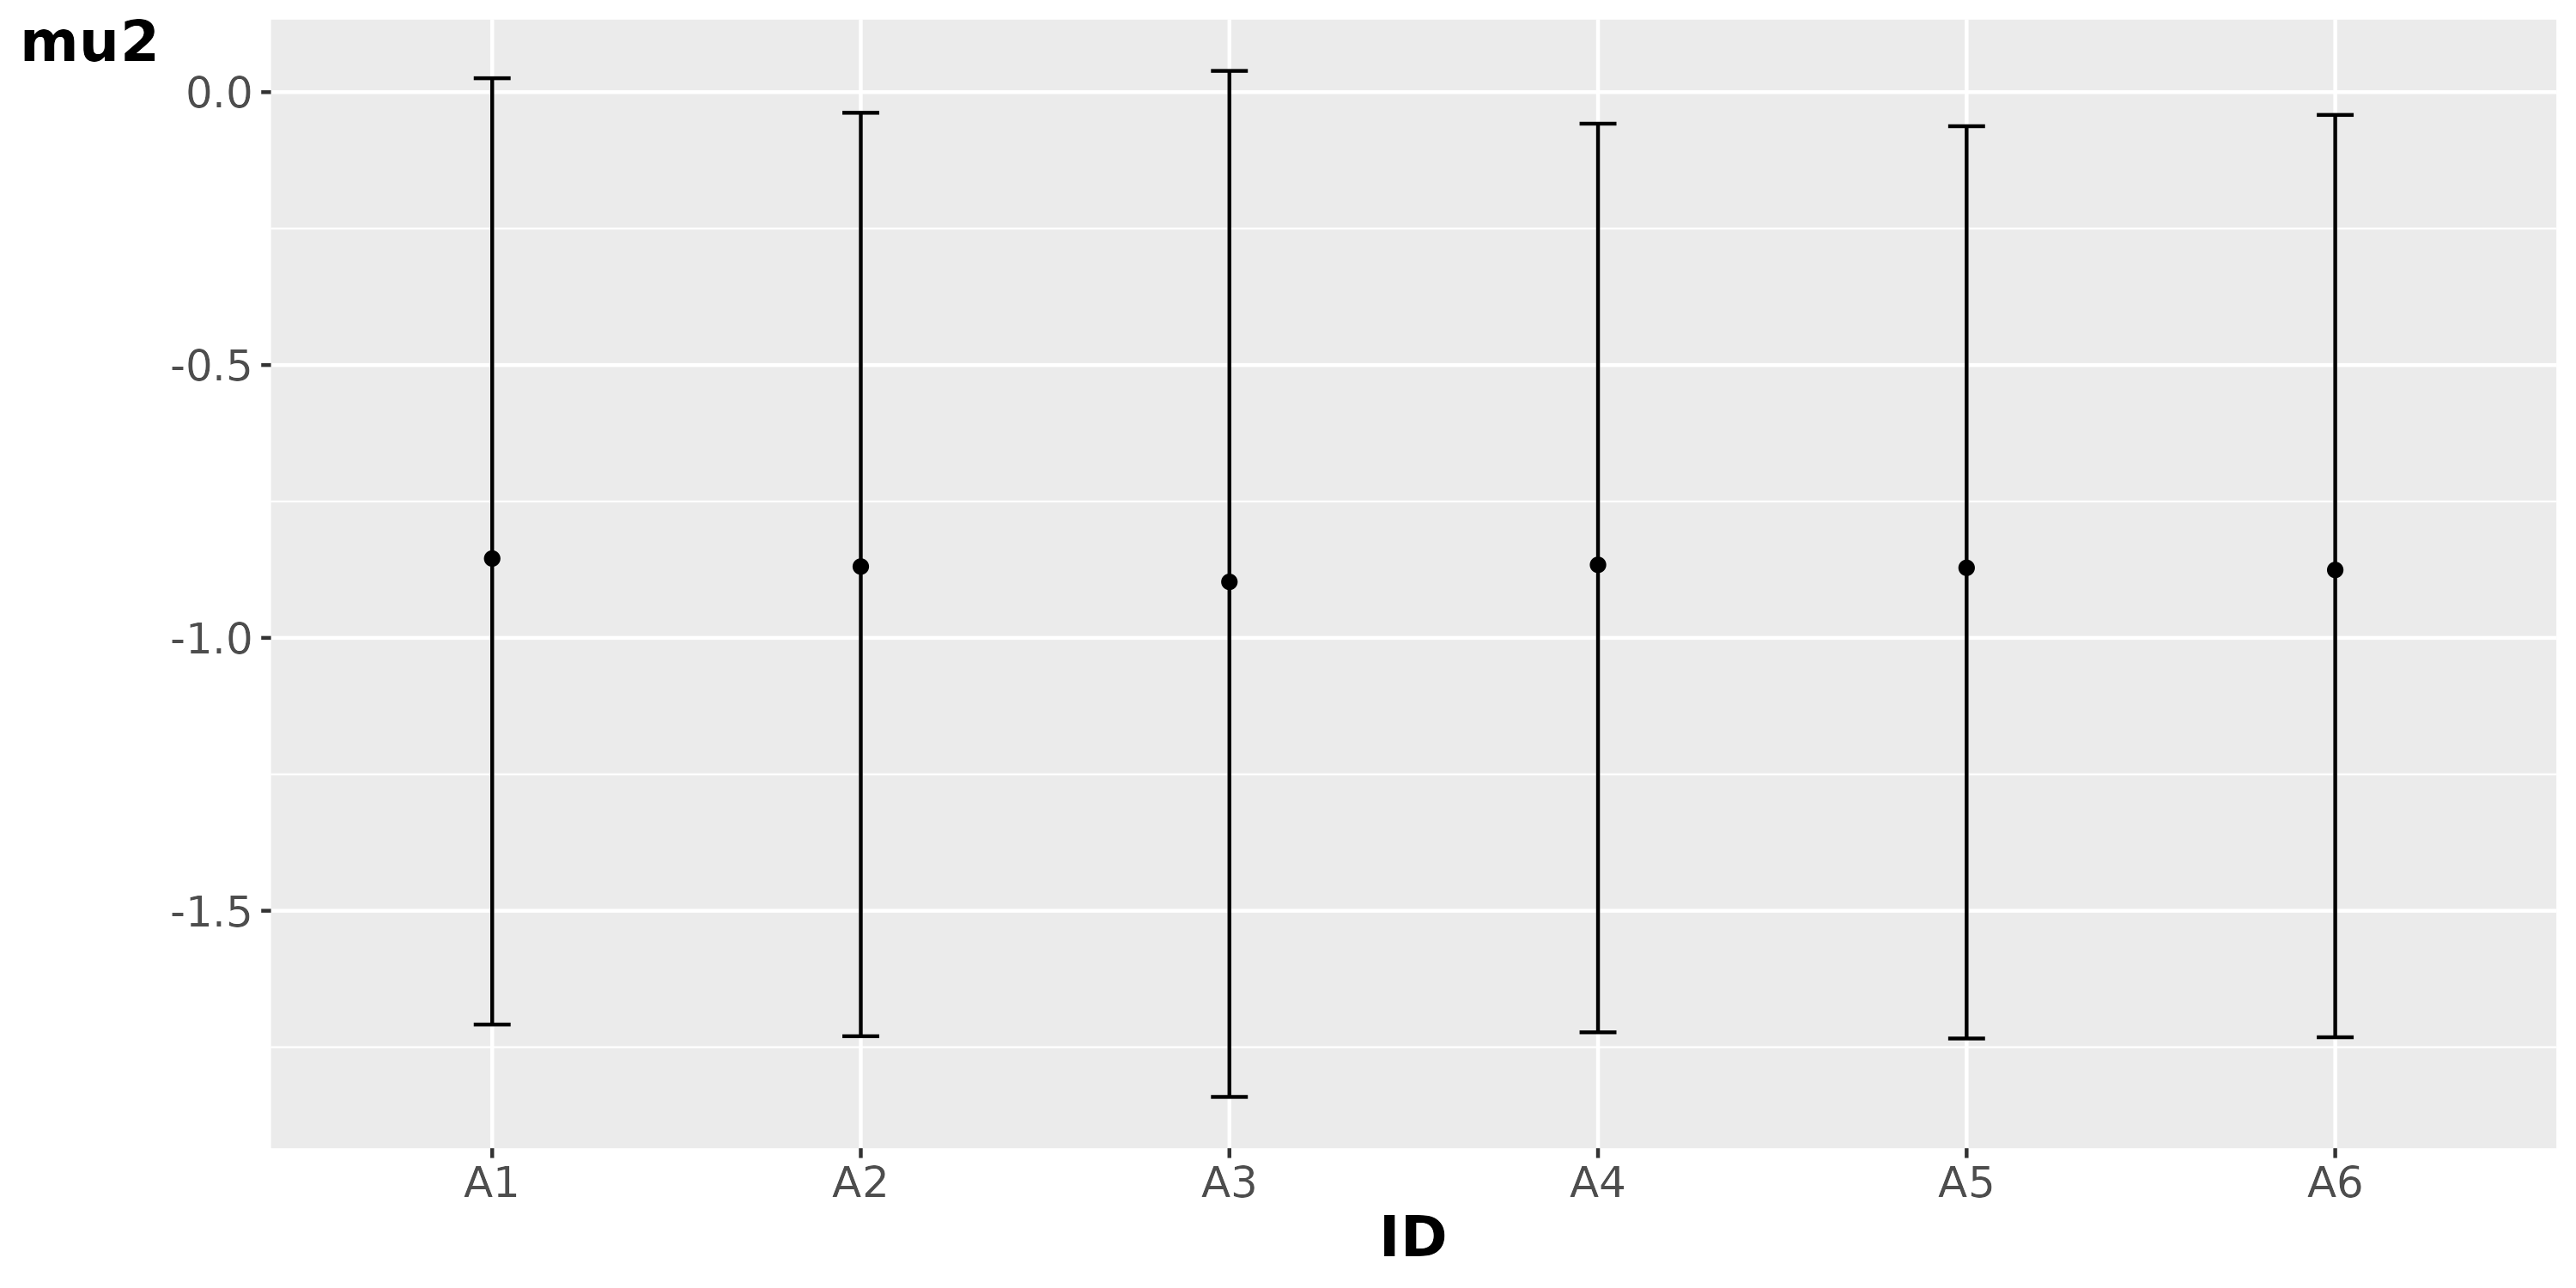
\includegraphics[scale=0.3]{images/unconstrained_models/baseline/re_baseline2_mu2.png}
    \caption{Estimated $\mu_2$ (km/h) for the baseline model}
    \label{fig: re_baseline1_mu2}
    \end{subfigure}
  	\begin{subfigure}{0.49\textwidth}
	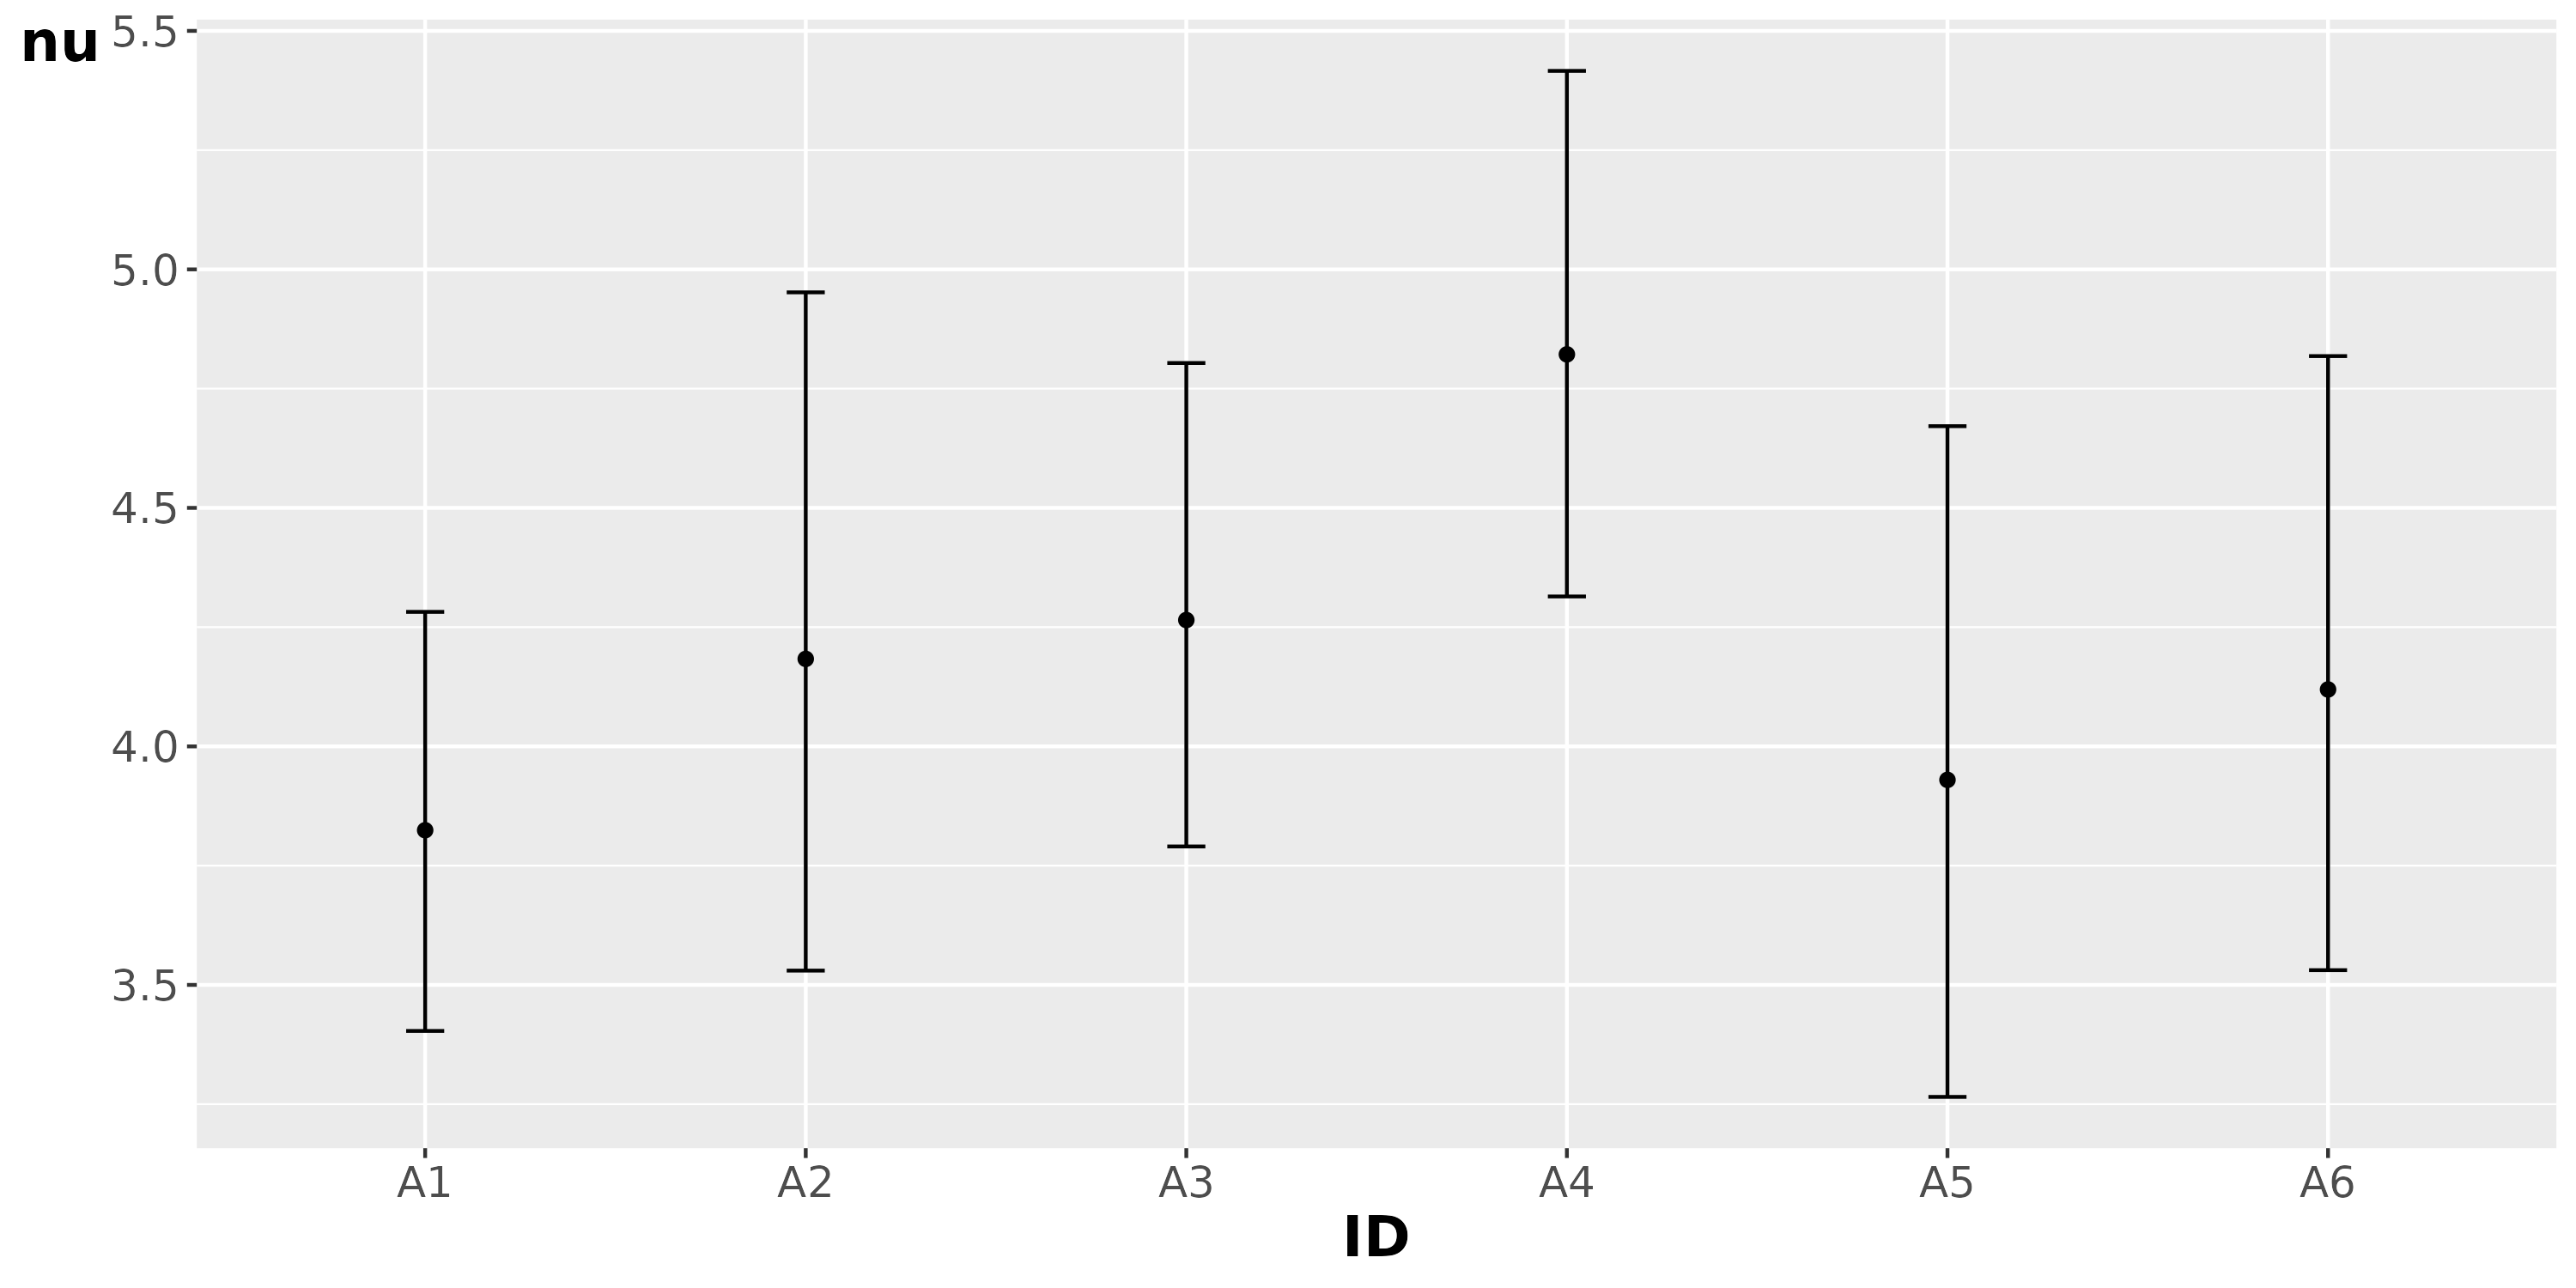
\includegraphics[scale=0.3]{images/unconstrained_models/baseline/re_baseline2_nu.png}
	\caption{Estimated $\nu$ (km/h)for the baseline model}
	\label{fig: re_baseline1_tau}
	\end{subfigure}
    \caption{Estimated parameters for each individual in the baseline model : the y axis are the estimated parameters along with $95 \%$ confidence interval and the x-axis represents the narwhals's ID.}
    \label{fig: constraints free baseline estimates}
\end{figure}

The estimated values for $\nu$ are all close to $4$ km/h with slight variations among individuals. This value should not be come as a surprise since the mean value of the horizontal velocity norm in the data is $4.4$ km/h, and it is known  that once the velocity process has reached stationarity (typically after $3\tau$), its norm follows a Rice distribution, whose mean is close to $\nu$ when $\vert\vert\mu\vert \vert$ is 
close to $0$.\\

The response model after exposure will be compared to this baseline model to assess any external effect on the narwhals's movement. Examining deviations from this baseline only makes sense when the model is reliable and describes well the narwhals's movement under normal conditions.
To check the goodness of fit of the baseline model, two statistics are computed from the observed tracks of each narwhal : mean velocity norm and the mean velocity phase. For the $i$-th narwhal, the mean velocity norm and phase are approximated as
\[\tilde{v}^{(i)}=\frac{1}{n_i-1}\sum_{j=1}^{n_i-1}  \tilde{v}^{(i)}_j \quad \tilde{\phi}^{(i)}=\frac{1}{n_i-1} \sum_{j=1}^{n_i-1} \widehat{(v_j^{(i)},e)} \mbox{ where } e=(1,0)\]
where $\tilde{v}^{(i)}_j=\frac{y_{j+1}^{(i)}-y^{(i)}_j}{\Delta^{(i)}_j}$, $n_i$ is the number of measurements, $y^{(i)}_j$ is the GPS position of the narwhal $i$ at time $t_j^{(i)}$ and $\Delta^{(i)}_j=t^{(i)}_{j+1}-t^{(i)}_j$.\\
Then the intercepts and modes of the random effects of the fitted baseline model are sampled 500 times from the posterior distribution using the joint covariance matrix produced by the optimization of the likelihood. Draws of the parameters of the SDE are deduced from the sampled coefficients and one trajectory is simulated for each narwhal according to the sampled parameters. For each simulated trajectory, mean of the norm and the phase of the velocity are estimated. This produces an histogram for each statistic (norm and phase) and each narwhal. If sampled tracks have enough similarities with the observed tracks, then the observed statistics should appear near the middle of the histograms. This checking procedure was introduced in \cite{michelot_continuous-time_2022}. Figures~\ref{fig: baseline velocity norm posterior check} and~\ref{fig: baseline velocity phase posterior check} show respectively the histograms of the mean velocity norm and the mean velocity phase.

 \begin{figure}[H]
    \centering
    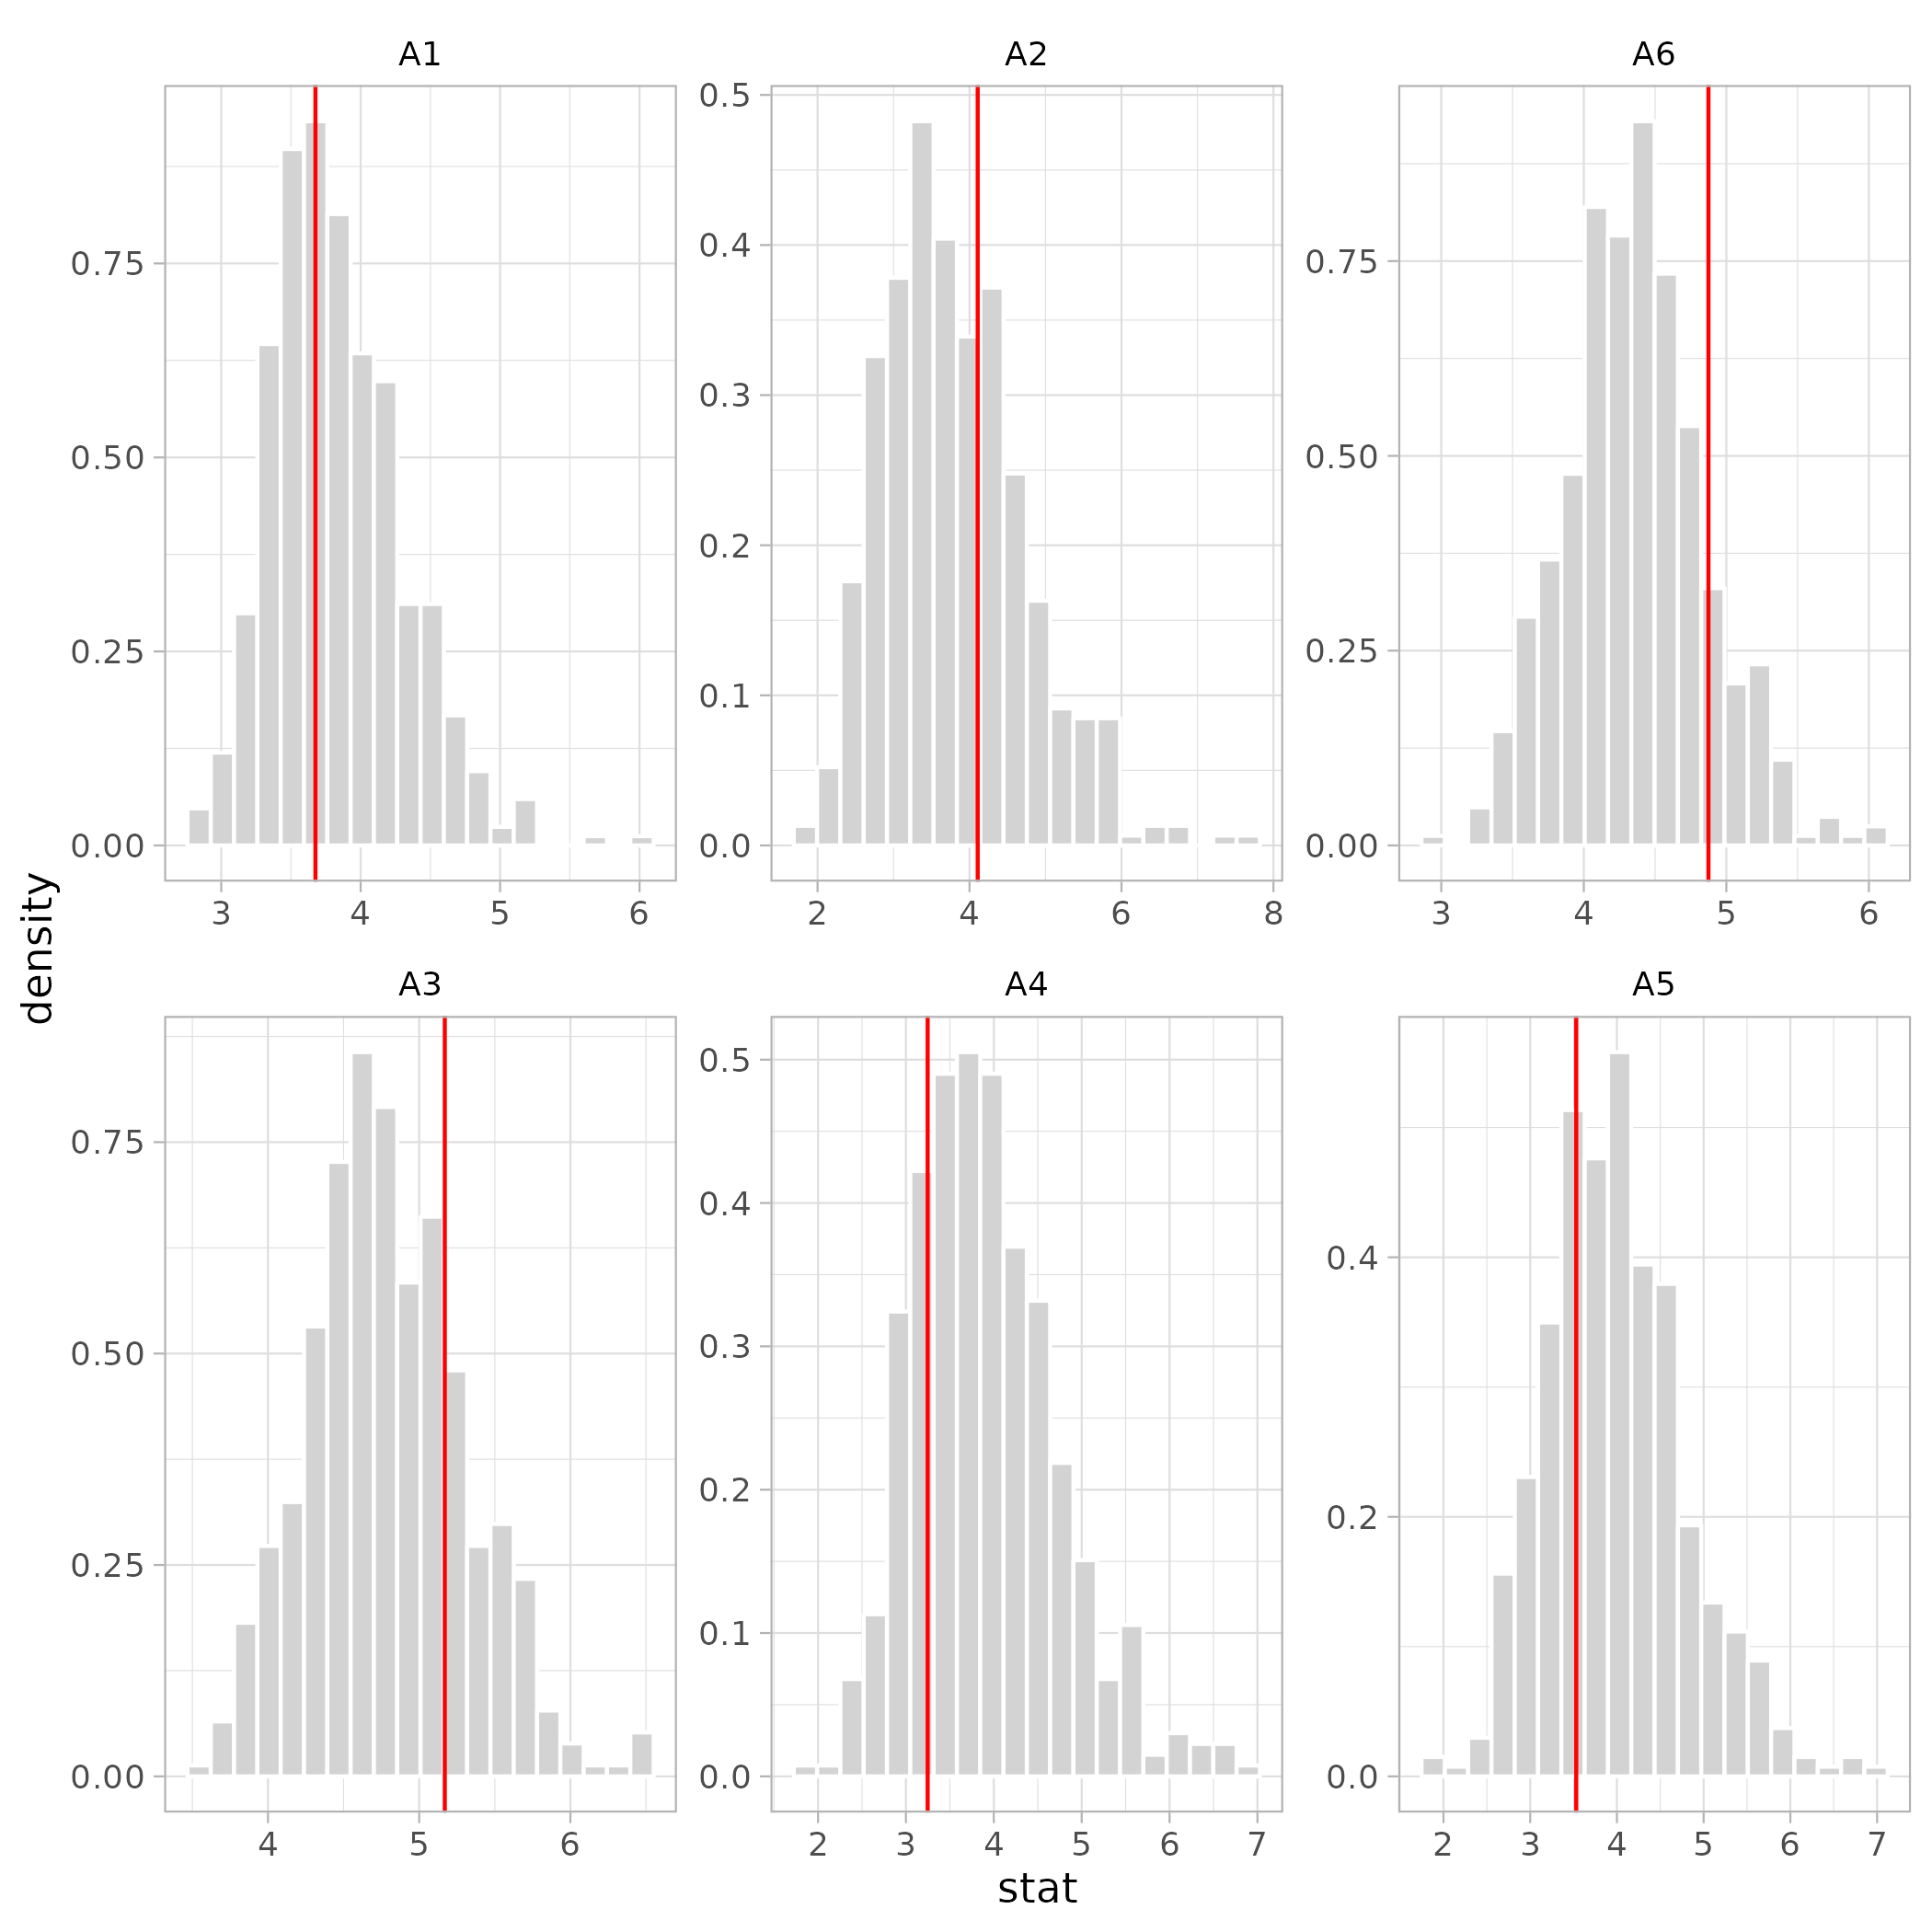
\includegraphics[scale=0.6]{images/unconstrained_models/baseline/check_mean_vnorm_baseline2.png}
    \caption{Histogram of the mean velocity computed from trajectories of the fitted model for each narwhal, along with observed values in red.}
    \label{fig: baseline velocity norm posterior check}
\end{figure}

 \begin{figure}[H]
    \centering
    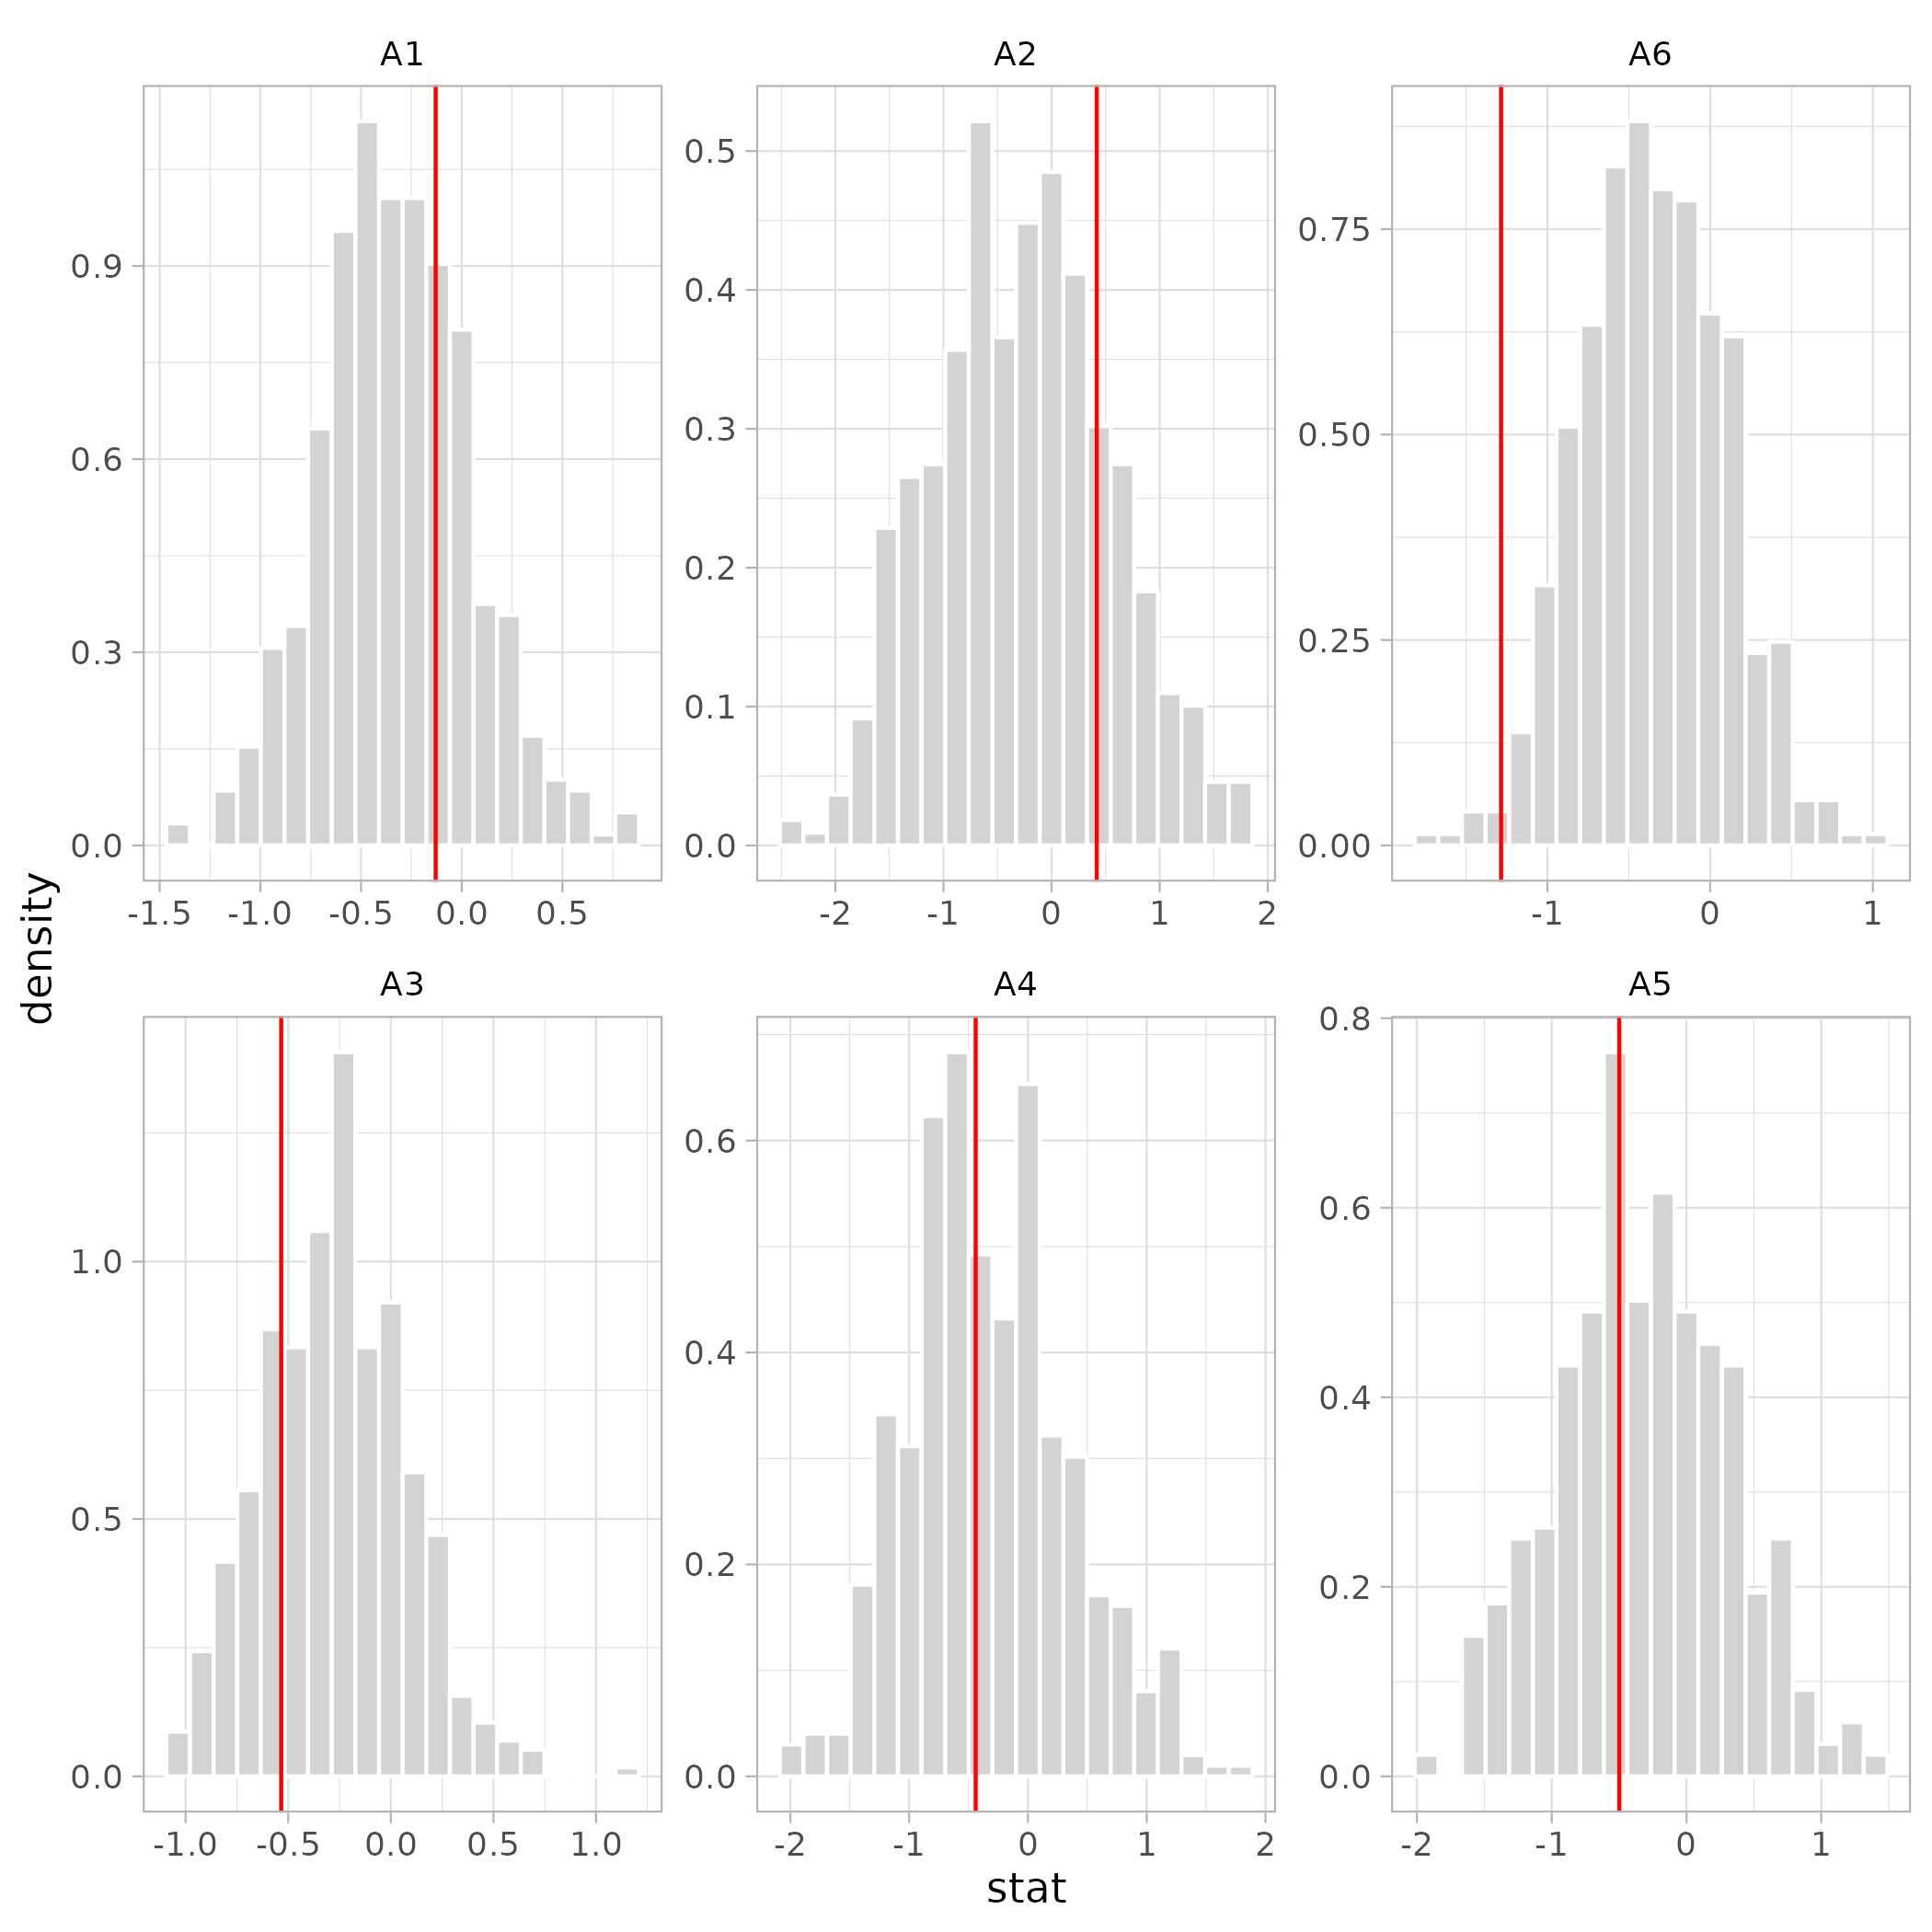
\includegraphics[scale=0.6]{images/unconstrained_models/baseline/check_mean_phase_baseline2.png}
    \caption{Histogram of the phase angle of the velocity computed from trajectories of the fitted model for each narwhal, along with observed values in red.}
    \label{fig: baseline velocity phase posterior check}
\end{figure}


The fitted baseline model seems to capture well the mean velocity norm and phase of the observed data for the majority of the narwhals. However, attention should be drawn on the phase angle histogram for the narwhal A6, which reveals a mismatch between the model and the observed phase angle. Narwhal A6 is likely to be heading in the south direction (mean phase angle close to $-\frac{\pi}{2})$. 


\paragraph{Response estimations}


Once the baseline model is deemed satisfactory, a response model is fitted on the tracks during exposure. We computed the marginal and conditional AIC values with different number of knotrs for the spline estimation of the parameters $\tau$ and $\nu$. The marginal AIC is defined in \cite{wood_generalized_2017} as $- 2L + 2k$ where L is the maximum marginal log-likelihood (of fixed effects), and $k$ is the number of degrees of freedom of the fixed effect component of the model. The conditional AIC also defined in \cite{wood_generalized_2017} is $- 2L' + 2k'$ where $L'$ is the maximum joint log-likelihood (of fixed and random effects), and $k'$ is the number of effective degrees of freedom of the model. Note that  the effective degree of freedom is not properly a number of degrees of freedom, but rather a measure of the flexibility or complexity of the model %detail how AIC is computed (wood); based on the trace of the Hessian matrix of the negative log likelihood.
%Intuition for the effective degreed of freedom
%Tendency to favour more complex model when the true model is not in the set of models tested

\begin{figure}[H]
	\centering
	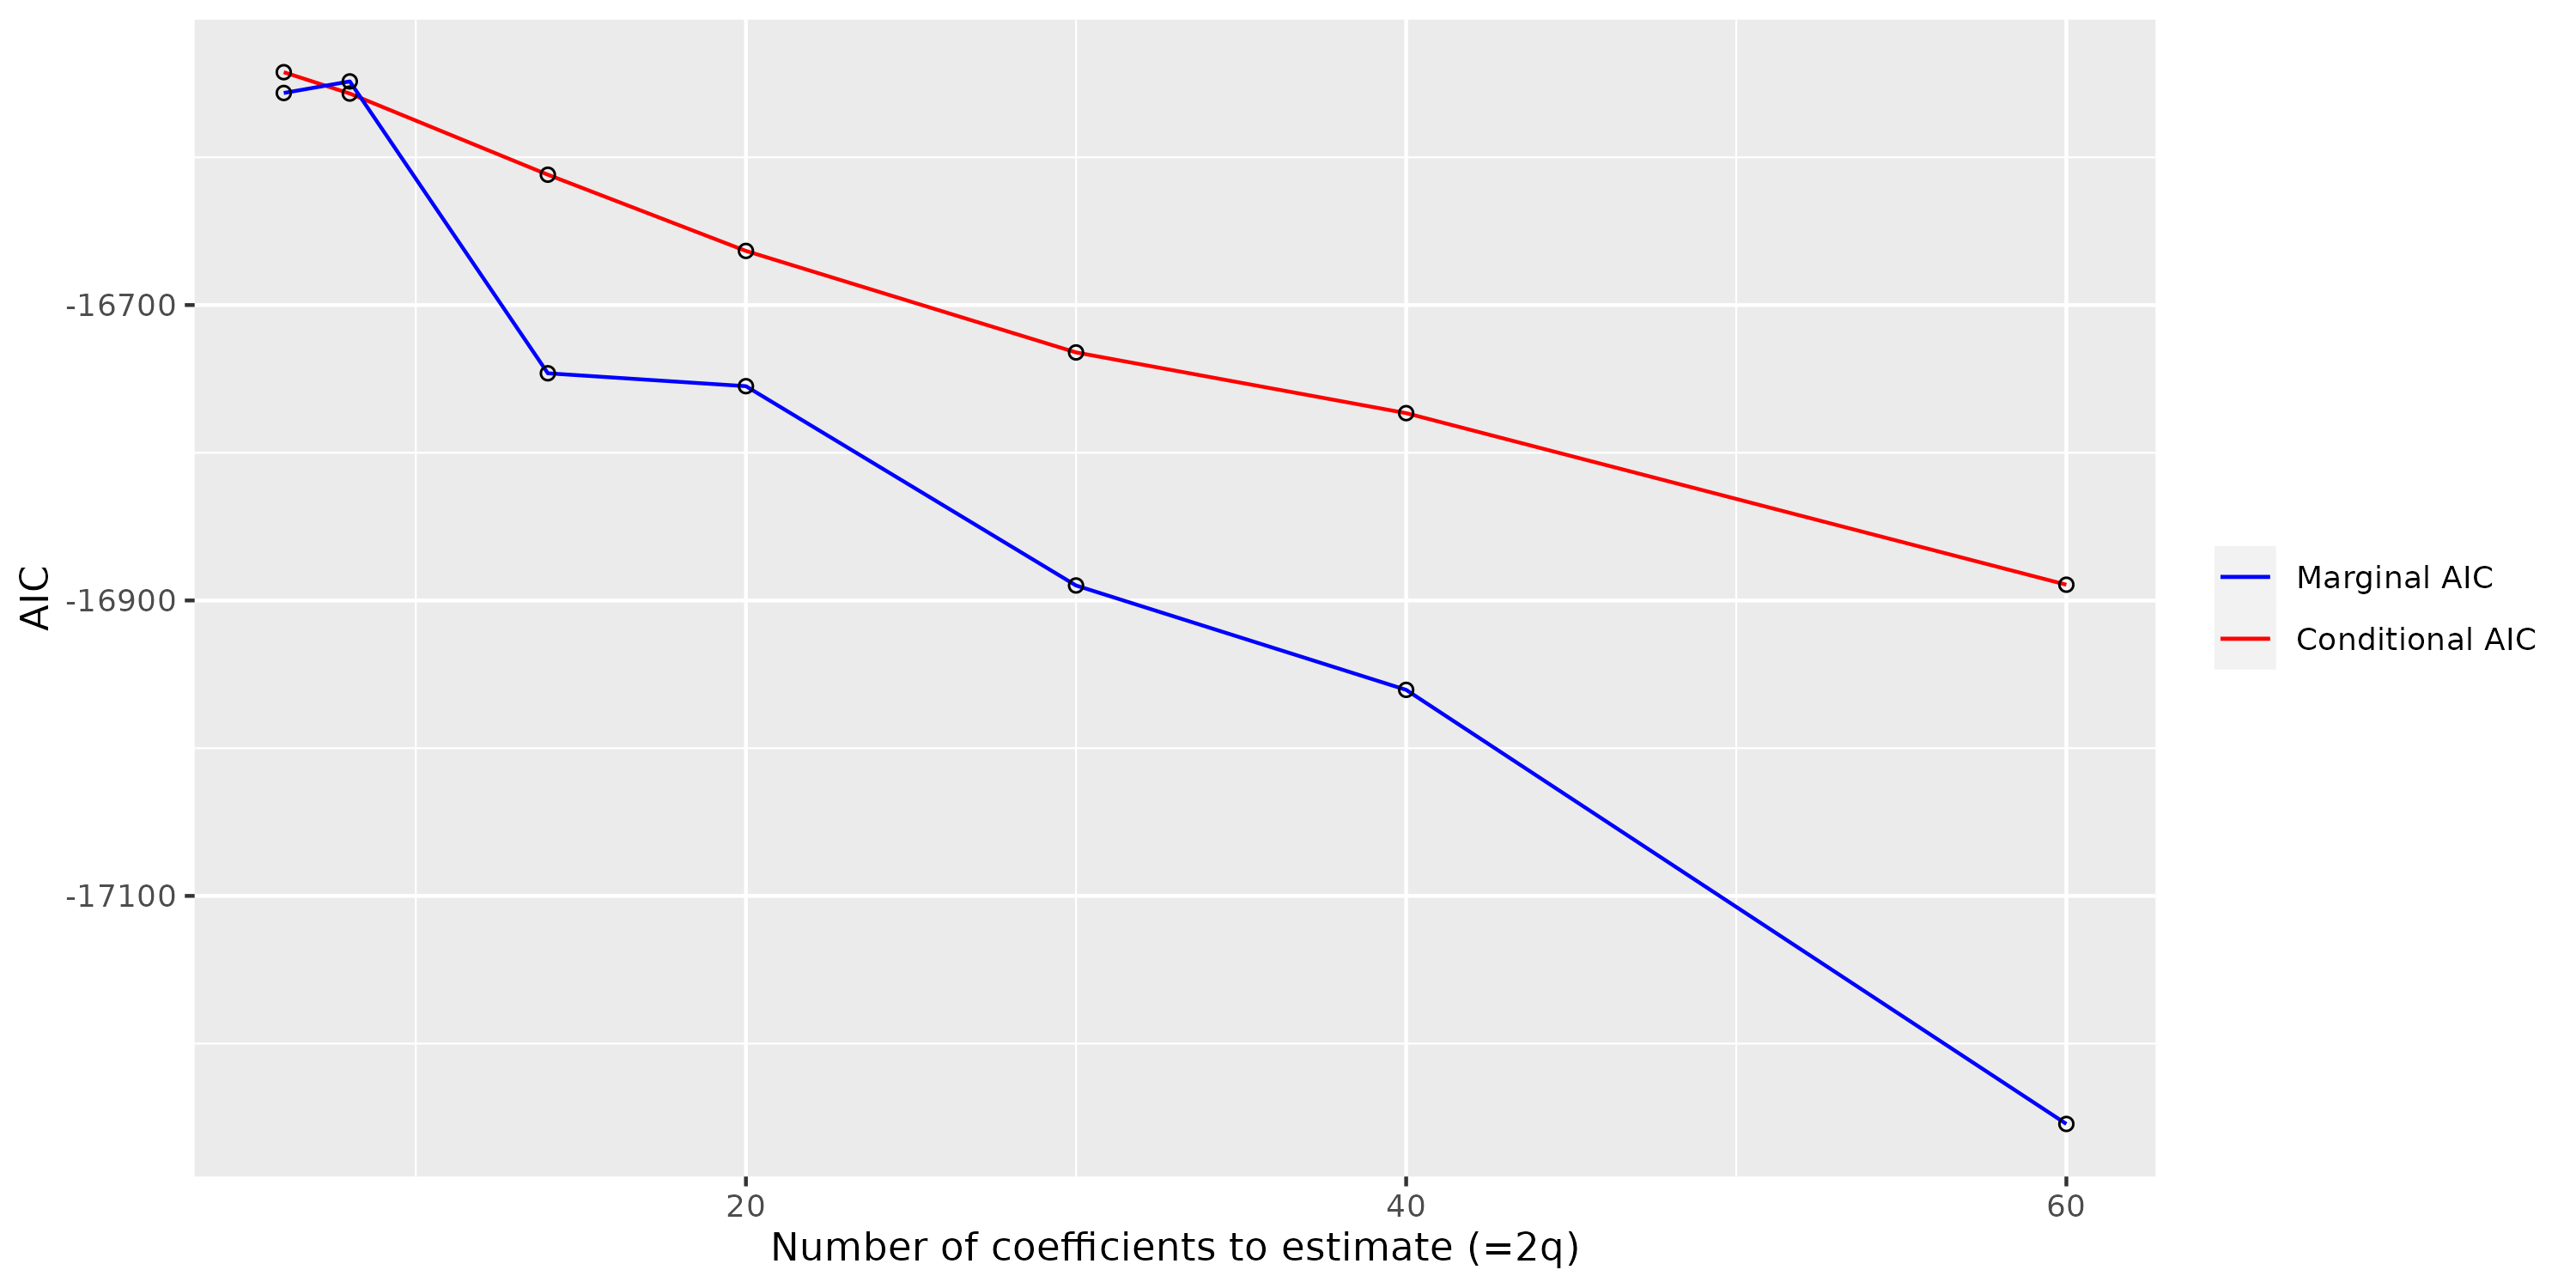
\includegraphics[scale=0.45]{images/unconstrained_models/response/plotAIC3.png}
	\caption{}
	\label{fig: plotAIC3}
\end{figure}

After $q=7$, the decrease in the marginal AIC curve seems to be lower than it was before. This suggests to choose $q-1=6$ knots for the estimation of the parameters with cubic spline. Note that choosing $q$ a bit lower or higher does not change dramatically the estimated smooth functions.
Figure~\ref{fig: fe_response3_tau_ExpShip} shows the estimated fixed effects of the covariate $E$ for the parameter $\tau$. Figure~\ref{fig: fe_response3_nu_ExpShip} shows the same plot but for the smooth parameter $\nu$. The variable on the x-axis is the distance to the shore, that is the inverse of $E$. 


\begin{figure}[H]
    \centering
    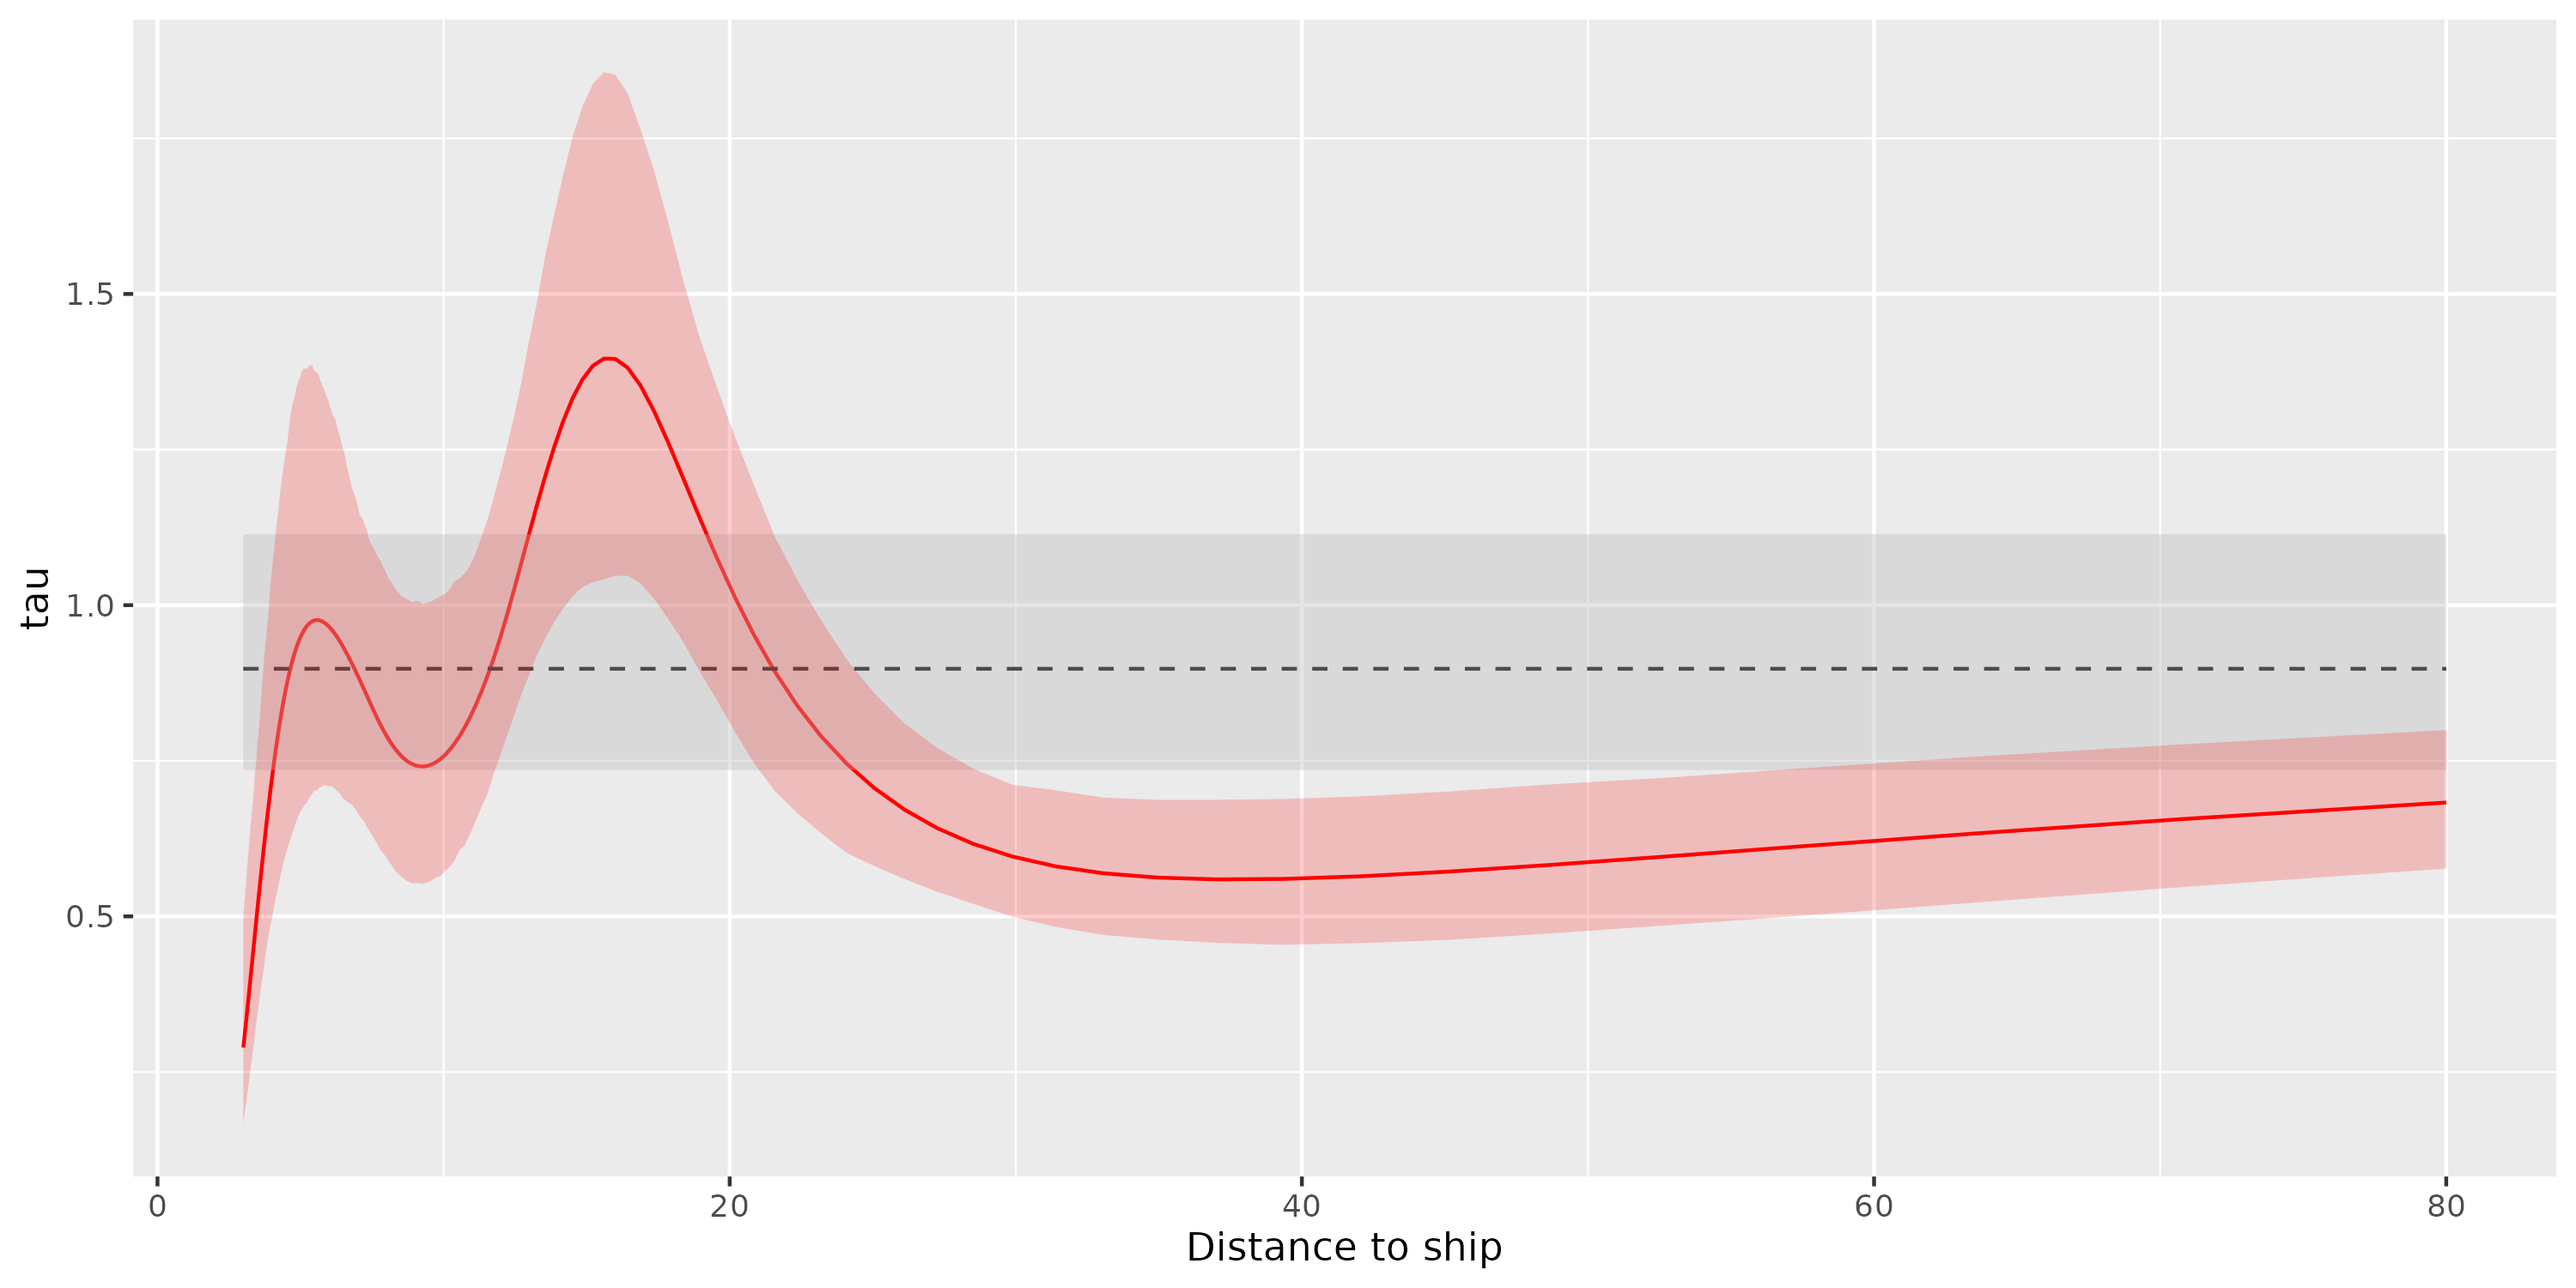
\includegraphics[scale=0.45]{images/unconstrained_models/response/fe_response3_tau_ExpShip.png}
    \caption{Estimation of the fixed effects for $\tau$ with 95\% pointwise confidence interval. The red curve is the estimated function, the dotted line is the intercept estimated in the baseline with its 95\% confidence interval in light grey.}
    \label{fig: fe_response3_tau_ExpShip}
\end{figure}

\begin{figure}[H]
	\centering
	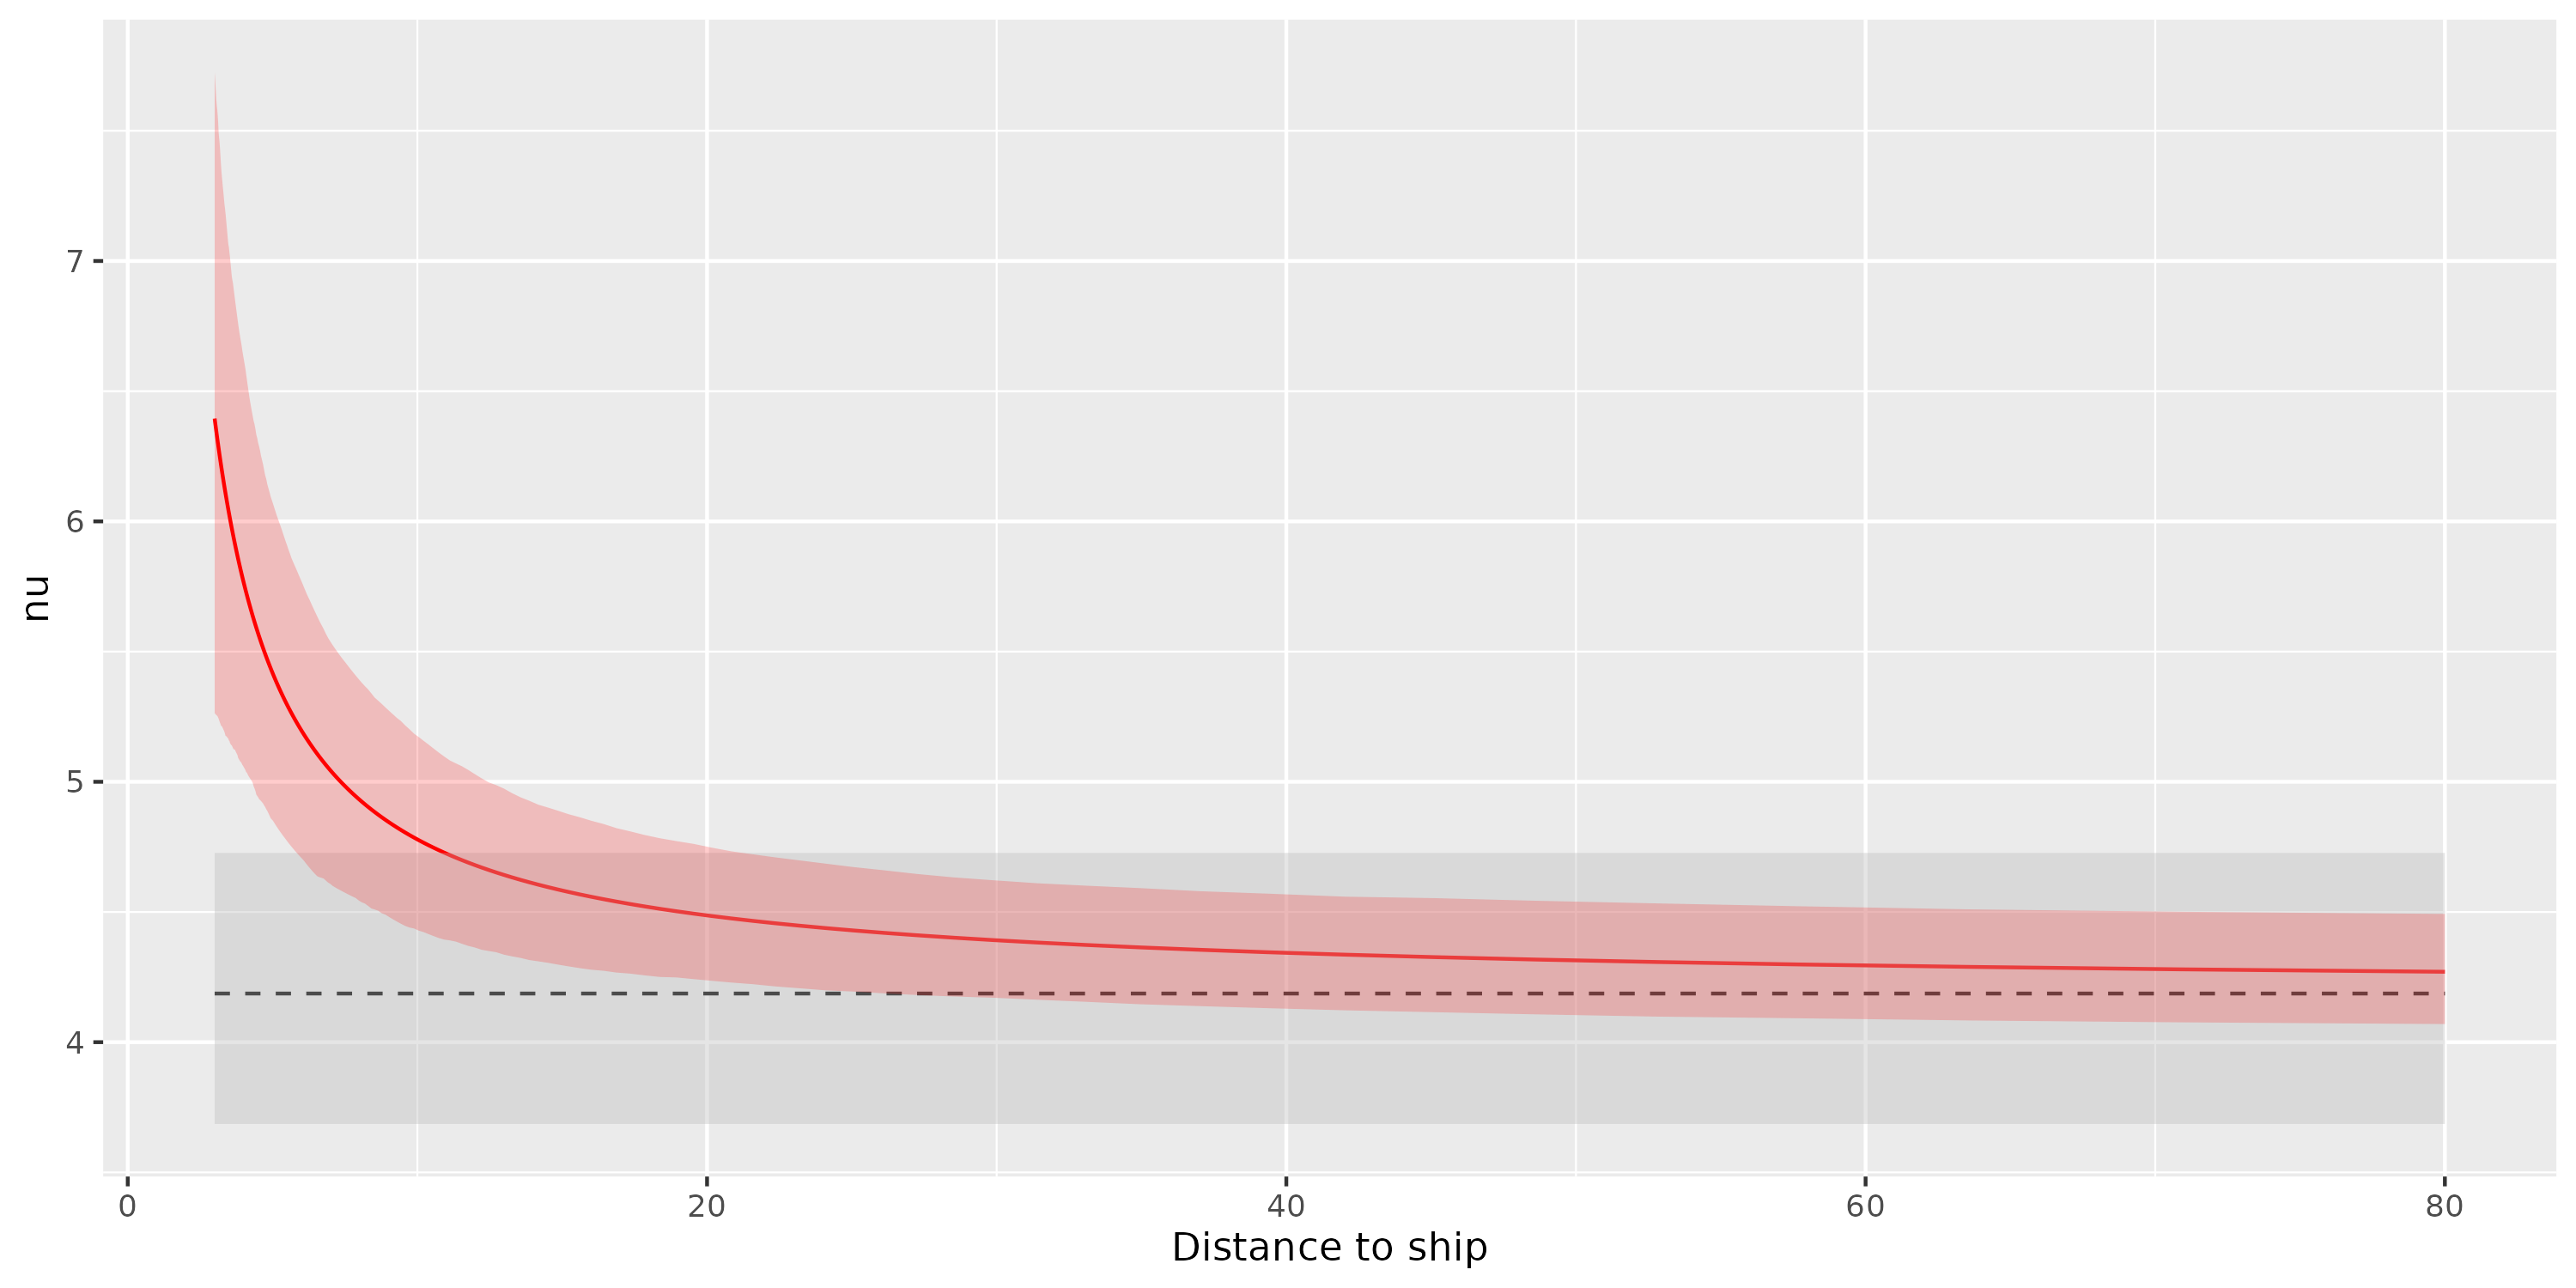
\includegraphics[scale=0.45]{images/unconstrained_models/response/fe_response3_nu_ExpShip.png}
	\caption{Estimation of the fixed effects for $\nu$ with 95\% pointwise confidence interval. The red curve is the estimated function, the dotted line is the intercept estimated in the baseline with its 95\% confidence interval in light grey.}
	\label{fig: fe_response3_nu_ExpShip}
\end{figure}

Deviations from undisturbed behaviour coincide with intervals on the x-axis where the confidence intervals of the baseline estimate and the response estimate are disjoint. 
This happens for the parameter $\nu$ when the narwhals are highly exposed to the ship, more precisely when they are at a distance to the ship lower than $8$ km. In this case, $\nu$ is significantly higher than the baseline value, proving that narwhals tend to move faster when highly exposed to the ship noise. Again, this should not come as a surprise since, for instance, the mean experimental velocity norm when the narwhals are less than $5$ km away from the ship is $5.7$ km/h, which is more than $1$ km/h higher than the mean experimental velocity norm before exposure. 
This also shows that the random component in the velocity equation has more importance when the narwhals are highly exposed to the ship, and can be interpreted as more variability in the narwhals horizontal velocity.
Regarding the persistence parameter, it is significantly lower than average in two cases. First, when the narwhals are very close to the ship (distance $<3.5$ km), it can be up to third times less persistent than usual. Then, up to $25$ km away from the ship, no significant deviation from the baseline value can be ascertained. However, more than $25$ km away from the ship, it can still be detected that the narwhals persistence is a bit lower than the baseline value (around $0.6$ instead of $0.9$). This decrease in persistence reveals that the animals gets generally agitated and have a tendency to change their heading more frequently when the military ship is sailing in the fjords.\\

Narwhals position relative to the ship were considered :
\begin{itemize}
	\item very close when the distance to the ship was lower than the $5\%$. quantile, which is $4.04$ km.
	\item close when the distance to the ship was lower than the $25\%$ quantile, which is $9.35$ km.
	\item medium when the distance to the ship was between the $25\%$ and $75\%$ quantile, that is between $9.35$ and $25.80$ km.
	\item far otherwise.
\end{itemize}
\begin{table}[H]
	\centering
\begin{tabular}{|c|c|c|c|c|}
	\hline
	Position relative to the coast & mean $\hat{\tau}$  & mean $\hat{\nu}$ & $\frac{\hat{\tau}-\hat{\tau}_{pre}}{\tau_{pre}}$ & $\frac{\hat{\nu}-\hat{\nu}_{pre}}{\hat{\nu}_{pre}}$   \\
	\hline
	Very close & 0.50 & 6.1 & $-44 \%$ & $+45 \%$ \\
	\hline
	Close & 0.88 & 5.3 & not significaant & $+26\%$ \\
	\hline
	Medium&  1.01 &  4.6 &  not significant & not significant \\
	\hline
	Far &  0.60 & 4.3 & $-33\%$ & not significant \\
	\hline
\end{tabular}
\caption{Comparison of response and baseline values of the parameters for different levels of exposure to the ship}
\label{table: baseline vs response parameters comparison}
\end{table}

\textcolor{red}{ADD POSTERIOR PREDICTIVE CHECKS}

\subsubsection{Estimation with constraints}



\paragraph{Baseline estimations}

The effect of the shore was included directly in the baseline model through bivariate splines of the Distance to the shore and the angle $\Theta$.
The mean velocity $\mu$ was fixed to $(0,0)$ and $\omega$ was estimated as smooth functions of $D_{shore}$ and $\Theta$.


\textcolor{red}{More details about tensor splines estimations can be found in chapter 4 of \cite{wood_generalized_2017}.}

\begin{figure}[H]
	\centering
	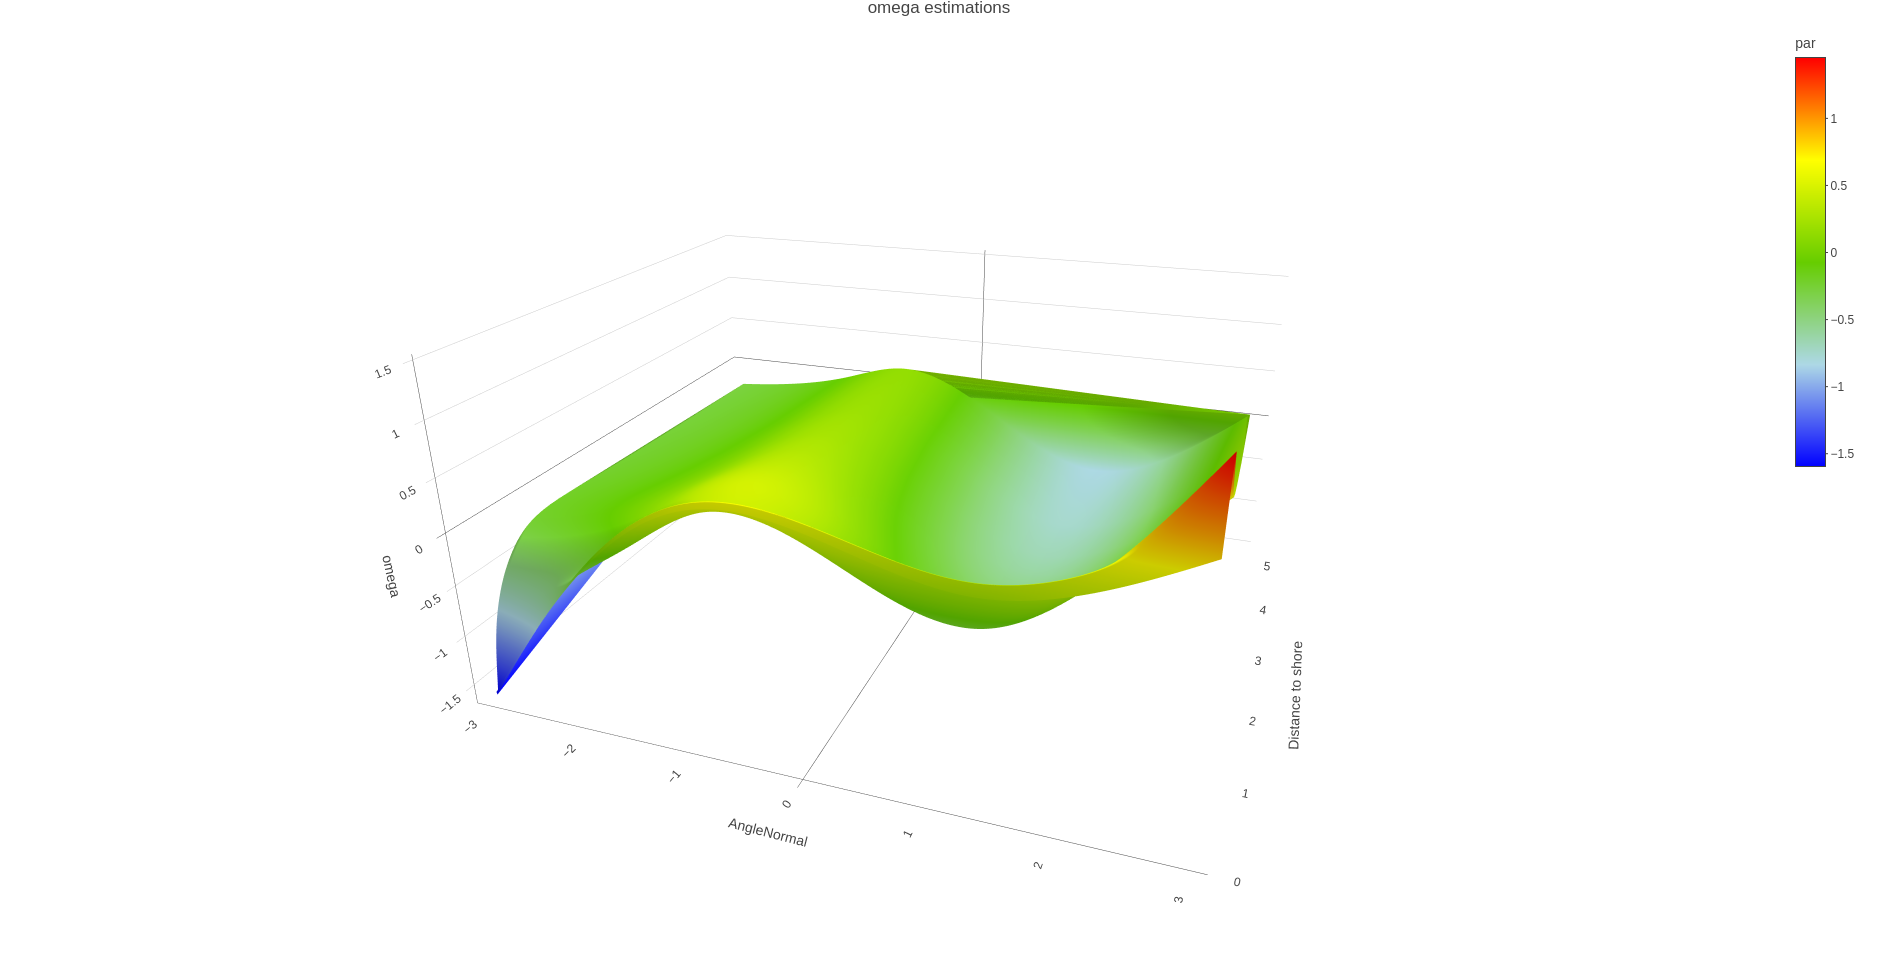
\includegraphics[width=0.7\linewidth]{images/application/omega_estimations}
	\caption{Estimation of smooth parameter $\omega$ with tensor splines}
	\label{fig:omegaestimations}
\end{figure}



\paragraph{Response estimations}
\end{comment}

\section{Discussion}


\textcolor{red}{Further work: 
\begin{itemize}
	\item Error in \texttt{smoothSDE} approximation based on the exact state space model, which is, in the case $\omega=0$ 
	\[
	\left\{
	\begin{array}{l}
		y_{c,j}=Z\alpha_{c,j}+\varepsilon_{c,j} \\
		\alpha_{c,j+1}=T_j \alpha_{c,j}+\begin{pmatrix} \Delta_j \\ 0 \end{pmatrix} \mu_c+\eta_{c,j} 
	\end{array}
	\right.
	\]
	where $Z=\begin{pmatrix} 1 & 0 \end{pmatrix}$, $\varepsilon_{c,j} \sim \mathcal{N}(0,H_{c,j})$, 
	$T_j=\begin{pmatrix} 
		1 & \int_{t_j}^{t_j+\Delta_j} e^{-I(v,j)}dv \\
		0 & e^{-I(t_j+\Delta_j,t_j)}
	\end{pmatrix}$  and $\eta_{c,j}=\begin{pmatrix} \xi_{c,j} \\ \zeta_{c,j} \end{pmatrix} \sim \mathcal{N}(0,Q_j)$ with
	\[Q_i=\begin{pmatrix}
		\int_{t_j}^{t_j+\Delta_j} \sigma(s)^2 \left(\int_{s}^{t_j+\Delta_j} e^{-I(v,s)} dv\right)^2 ds
		& \int_{t_j}^{t_j+\Delta_j} \sigma(s)^2e^{-I(t_j+\Delta_j,s)} \int_s^{t_j+\Delta_j} e^{-I(v,s)} dv ds \\
		\int_{t_j}^{t_j+\Delta_j} \sigma(s)^2e^{-I(t_j+\Delta_j,s)} \int_s^{t_j+\Delta_j} e^{-I(v,s)} dv ds & \int_{t_j}^{t_j+\Delta_j} \sigma(s)^2 e^{-2I(t_j+\Delta_j,s)} ds
	\end{pmatrix}
	\]
	and $I(t,s)=\int_{s}^{t} \beta(u) du$.
	How to control the error between these integrals and the approximated covariance matrix in \texttt{smoothSDE} ?
	\item Proof that the process $X$ in section~\ref{section: CRCVM} is constrained for simple domains (infinite vertical or horizontal barrier, rectangle for instance) which involves the diameter of rotation $\Leftrightarrow$ proof that the process $D^{shore}(t)$ is strictly positive (something like the non negativity condition for the CIR process ?)
\end{itemize}}

\begin{comment}
As discussed in \cite{ditlevsen_hypoelliptic_2019}, estimation for such hypoelliptic models is challenging. The main difficulties come from
\begin{itemize}
	\item degenerate noise structure that prevents the use of standard approximation schemes as Euler-Maruyama.
	\item irregular times of observations : we only get position when the marine mammal reaches the sea surface.
	\item GPS measurement errors, with gaussian or student distribution.
	\item partial observations : two processes are involved in equation~\ref{eq: RACVM equation}, however only one of them is observed, that is the position.
\end{itemize}
Several method already exist to estimate the parameters $\tau$, $\nu$, $\mu$ and $\omega$.
If the parameters are constant, it is possible to use a method of moments based on the distributional results about the velocity process \cite{gurarie_correlated_2017}, but it is only feasible with high frequency data and negligible measurement errors. Maximum likelihood with Kalman filter allows to estimate more efficiently from observations with errors \cite{johnson_continuoustime_2008}.
If the parameters are allowed to depend on time through external covariates, then \texttt{smoothSDE} package, which is based on \cite{johnson_continuoustime_2008} but exploit the capabilities of both the \texttt{mgcv} package \cite{wood_generalized_2017} to specify the time dependency through covariates, and the \texttt{TMB} \cite{kristensen_tmb_2016} package to integrate over the random effect and optimize the likelihood, is a convenient tool for estimation. \\


For the narwhals, a tendency to move along the shore could be considered by specifying a function $\omega$ that is non zero even when $\Theta \in \left[\frac{\pi}{2}-\varepsilon,\frac{\pi}{2}\right] \cup \left[-\frac{\pi}{2},-\frac{\pi}{2}+\varepsilon\right]$, so that when the animal would be on the verge of leaving the shore, its velocity would be tweaked to align with the shoreline. It is also possible  to specify $\tau$ similarly as a function of $D_{shore}$ and $\Theta$ to model specific behaviour near the shore (e.g higher persistence along the shoreline).
\end{comment}

\newpage

\printbibliography

\newpage 

\appendix

\section{More details about the data}

The median time step between GPS measurements is $4.8$ minutes, and the mean time step is $9.3$ minutes. The histogram of the time steps is shown in figure~\ref{fig:alltimestepshisto}.

\begin{figure}[H]
	\centering
	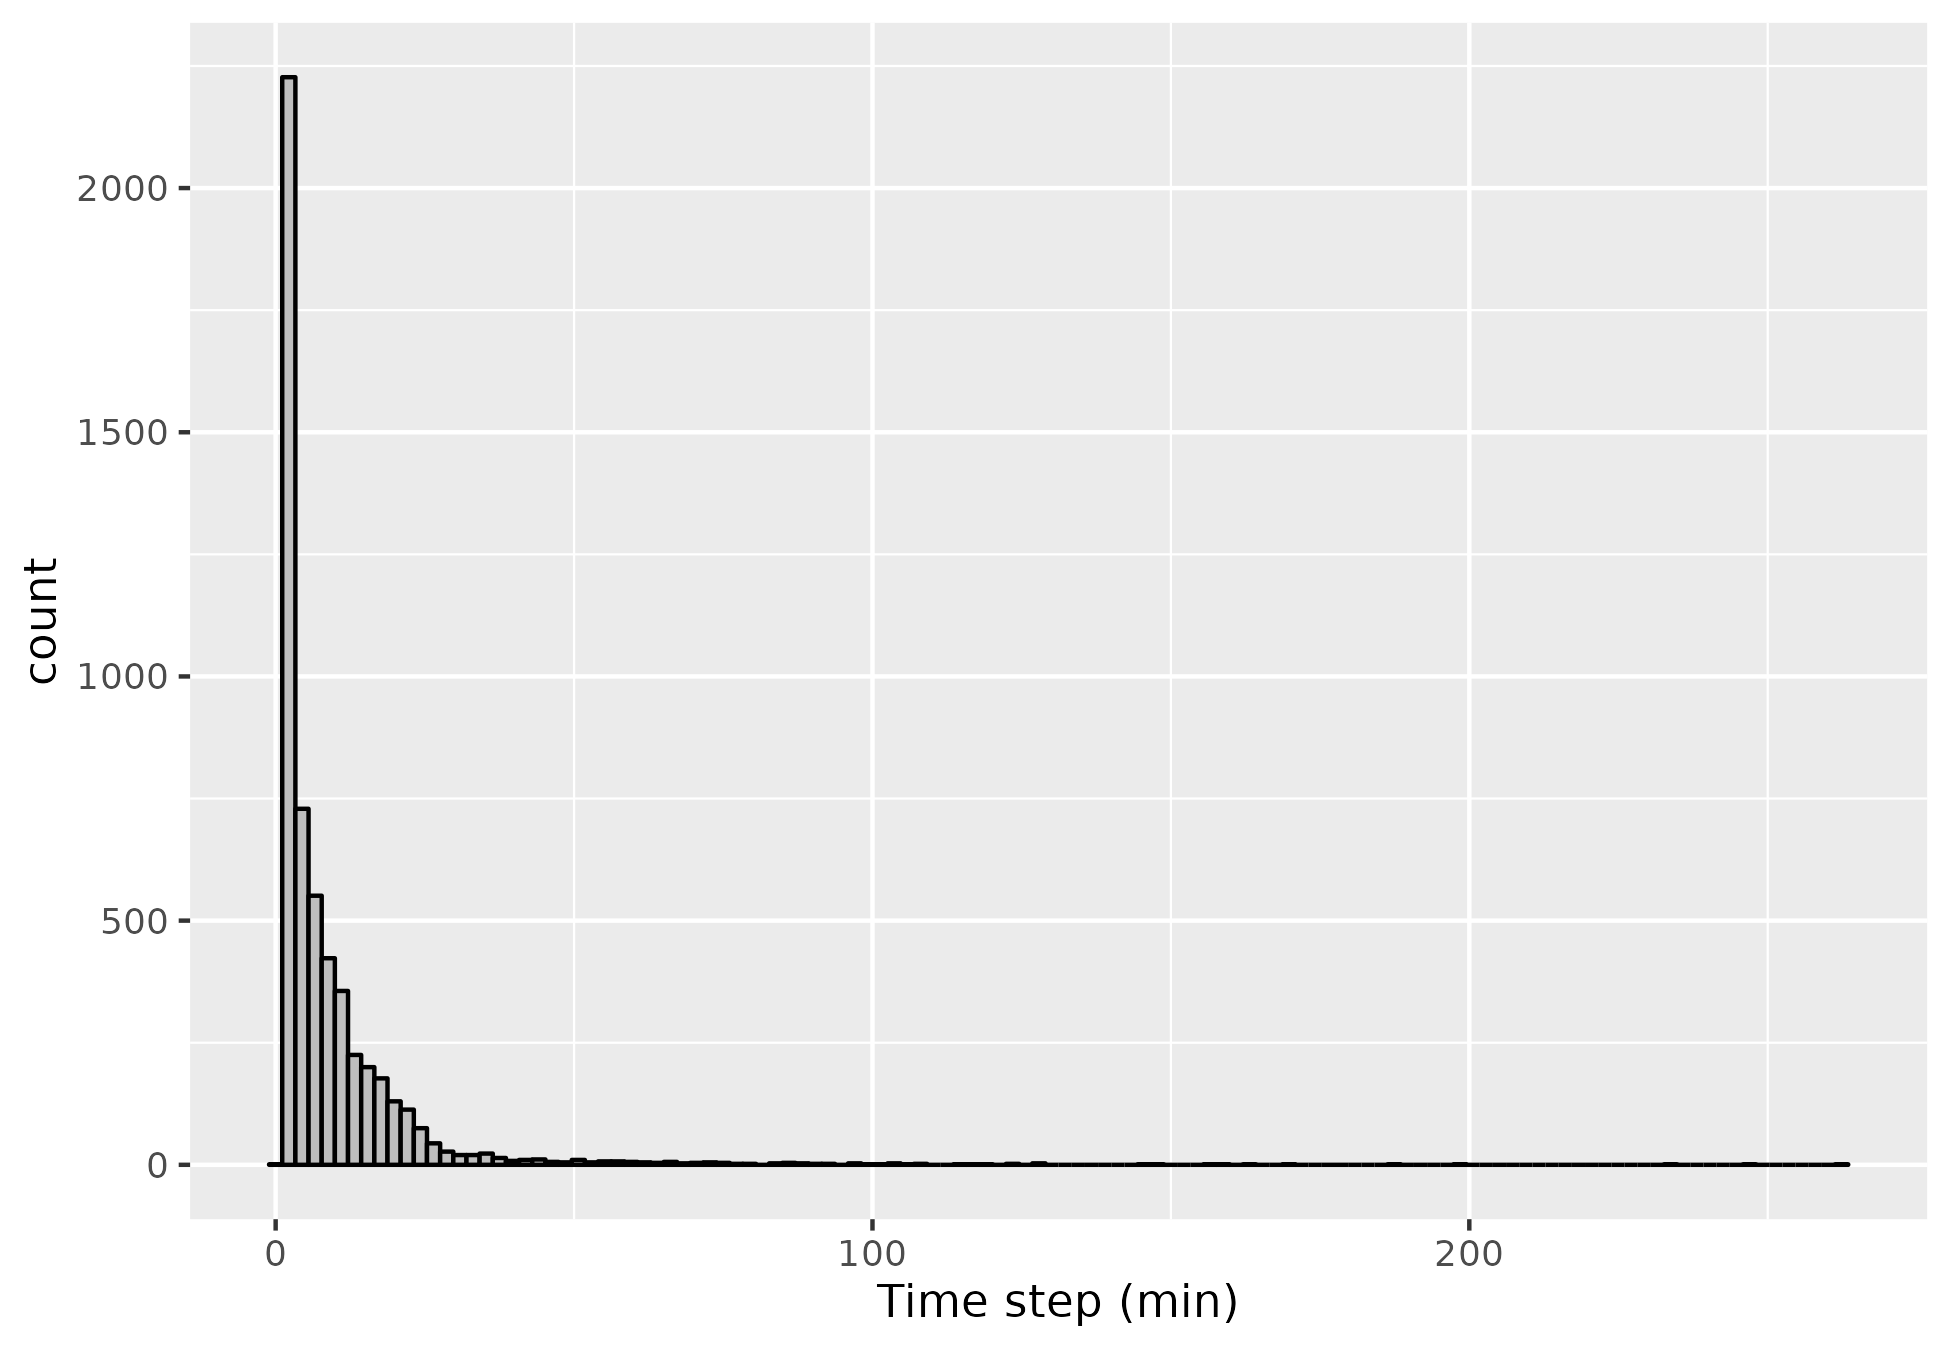
\includegraphics[scale=0.5]{images/data_exploration/all_time_steps_histo}
	\caption{Histogram of time steps}
	\label{fig:alltimestepshisto}
\end{figure}

Figure~\ref{fig: trials and intertrials distributions} shows how the exposure periods are distributed among the $6$ narwhals that were tracked. 

	\begin{figure}[H]
		\centering
			\centering
			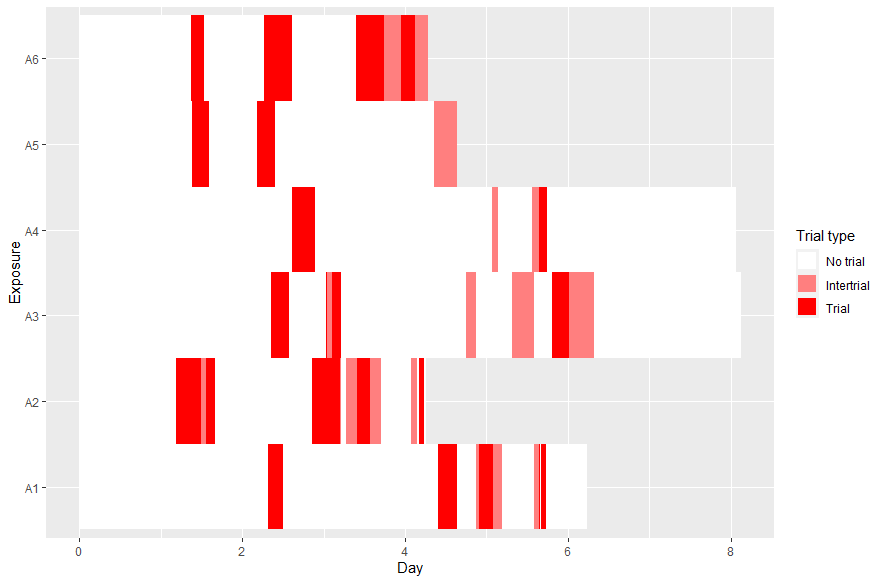
\includegraphics[width=0.9\textwidth]{images/data_exploration/trials.png}
			\caption{Trial and Intertrial periods for each narwhal}
			\label{fig: trials and intertrials distributions}
		
	\end{figure}
 
 Table~\ref{table: data distribution}  shows how the data is distributed among the different narwhals. Figure~\ref{fig: tracks before and after exposure} shows all the tracks before and after exposure on a map of Scoresby Sound fjords system.

\begin{table}[H]
	\centering
	\begin{tabular}{|c|c|c|}
		\hline
		Narwhal ID & Number of measurement before exposure & Number of measurements during exposure \\
		\hline
		A1 & 258 & 576\\
		\hline
		A2  & 40 & 515 \\
		\hline
		A3 & 222 & 680 \\
		\hline
		A4 & 291 & 642  \\
		\hline
		A5 & 48 & 419\\
		\hline
		A6 & 76 & 425 \\
		\hline
		\textbf{Total} & \textbf{935} & \textbf{3257} \\
		\hline
	\end{tabular}
	\caption{Distribution of the data among the 6 individuals}
	\label{table: data distribution}
\end{table}

\begin{figure}[H]
	\centering
	\begin{subfigure}{0.49\textwidth}
		\centering
		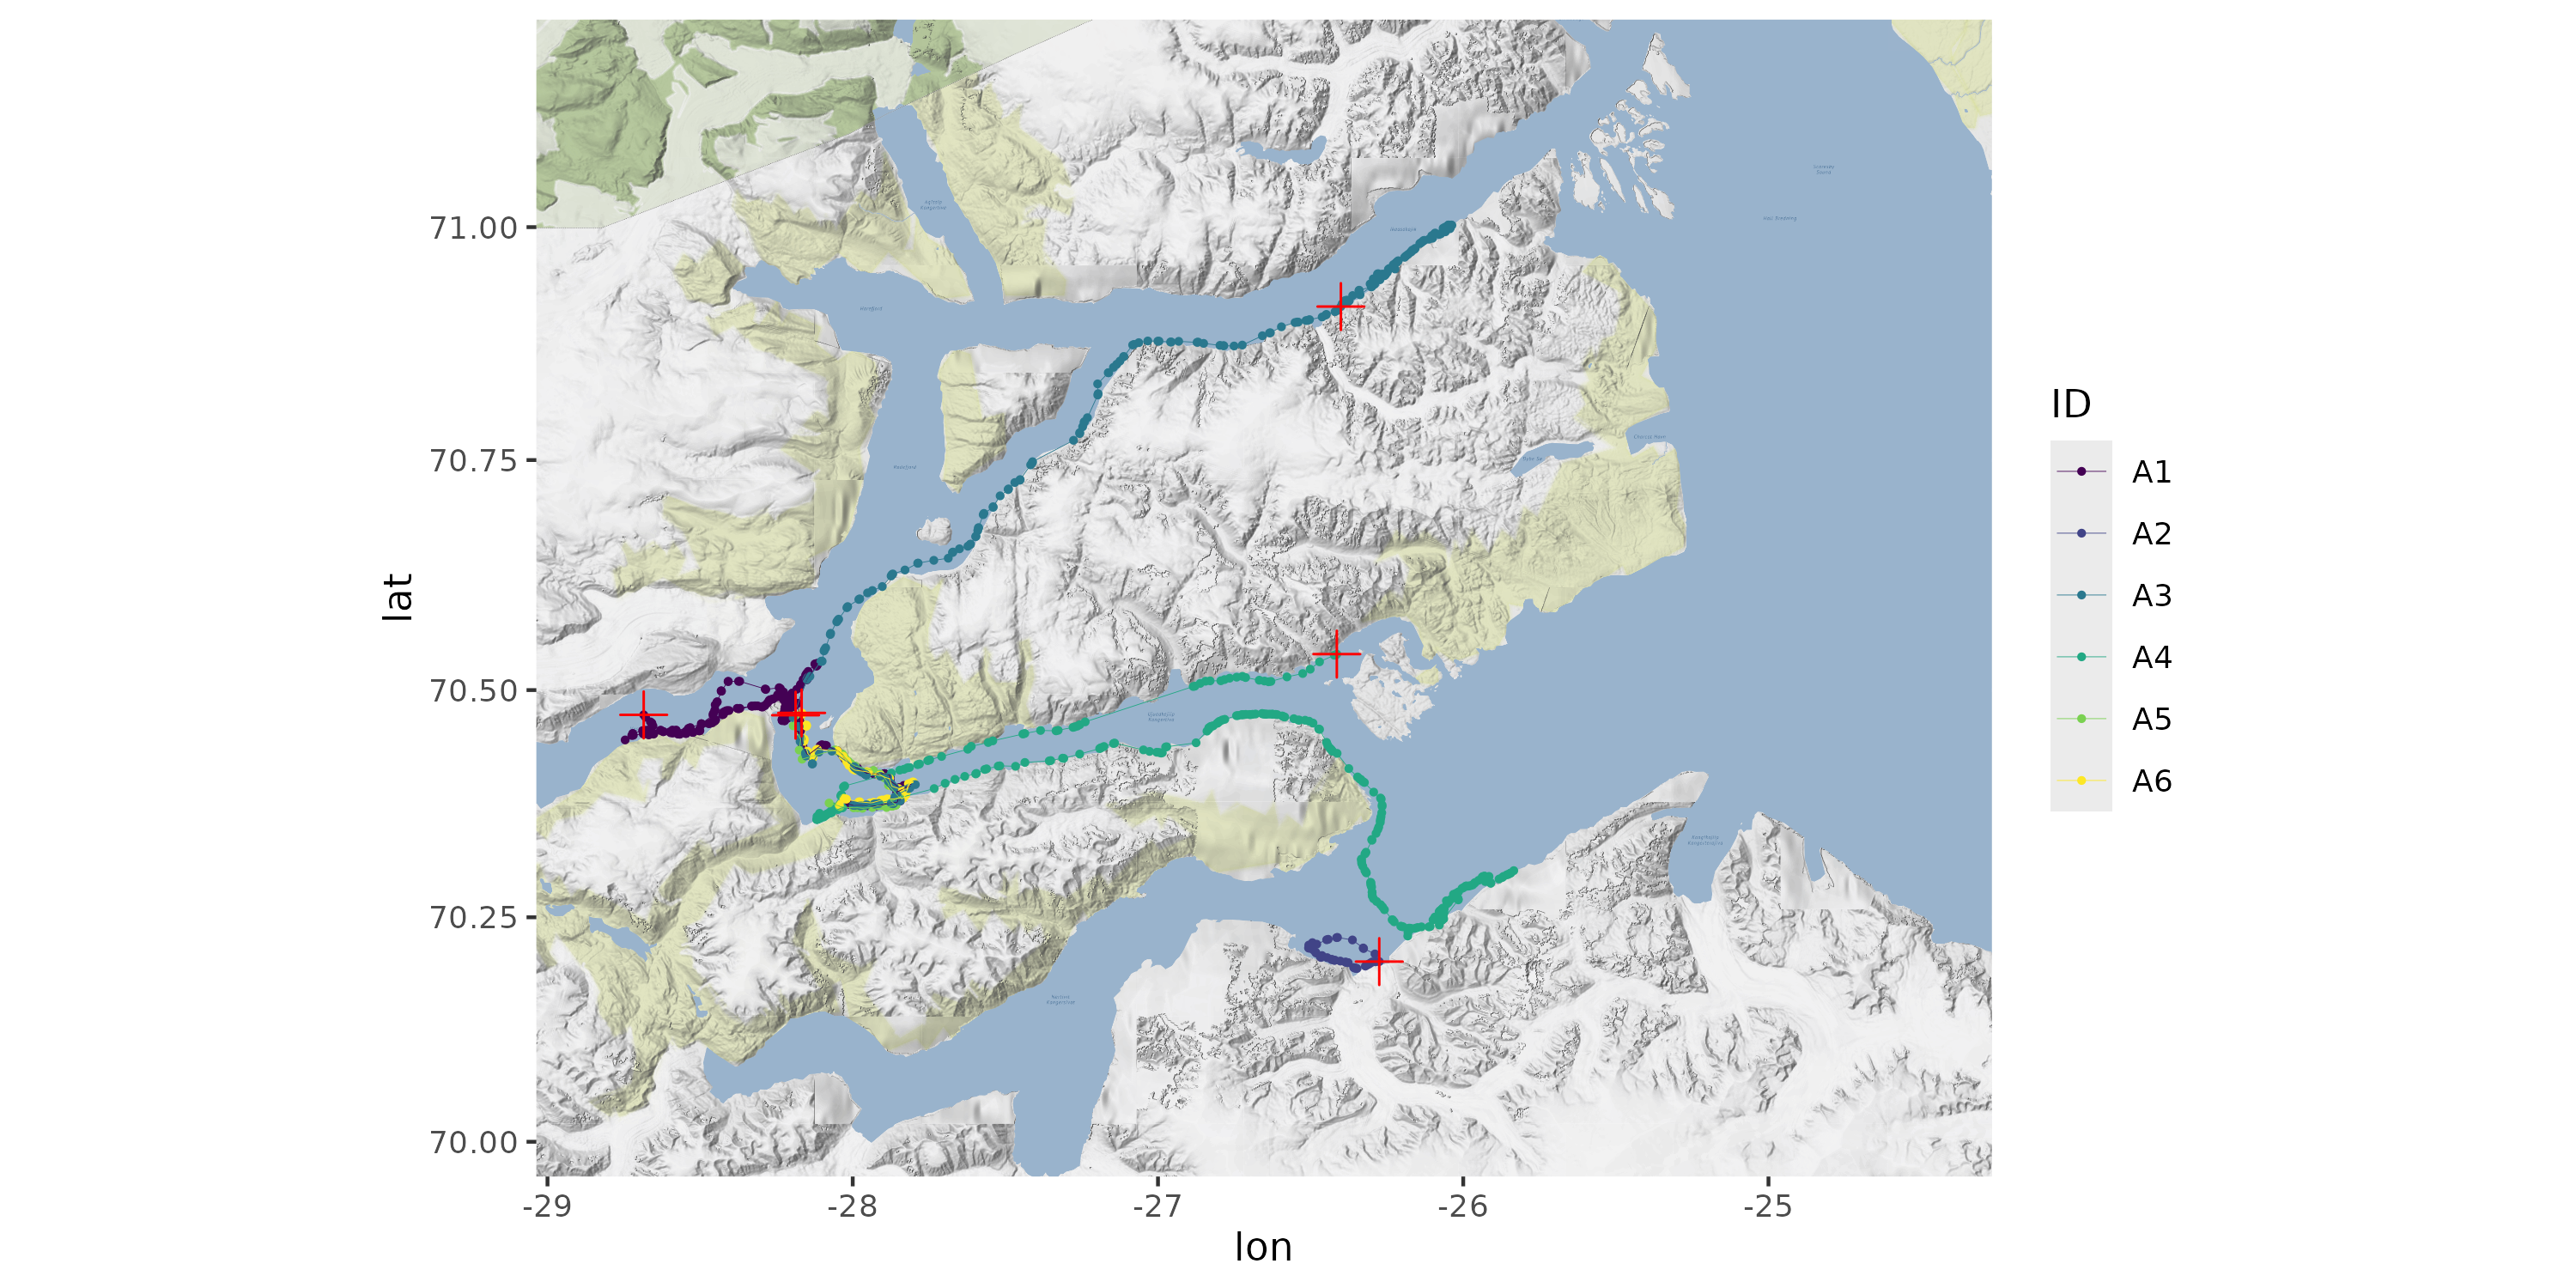
\includegraphics[scale=0.38]{images/data_exploration/tracksBE1.png}
		\caption{Tracks before exposure experiments}
	\end{subfigure}
	\begin{subfigure}{0.49\textwidth}
		\centering
		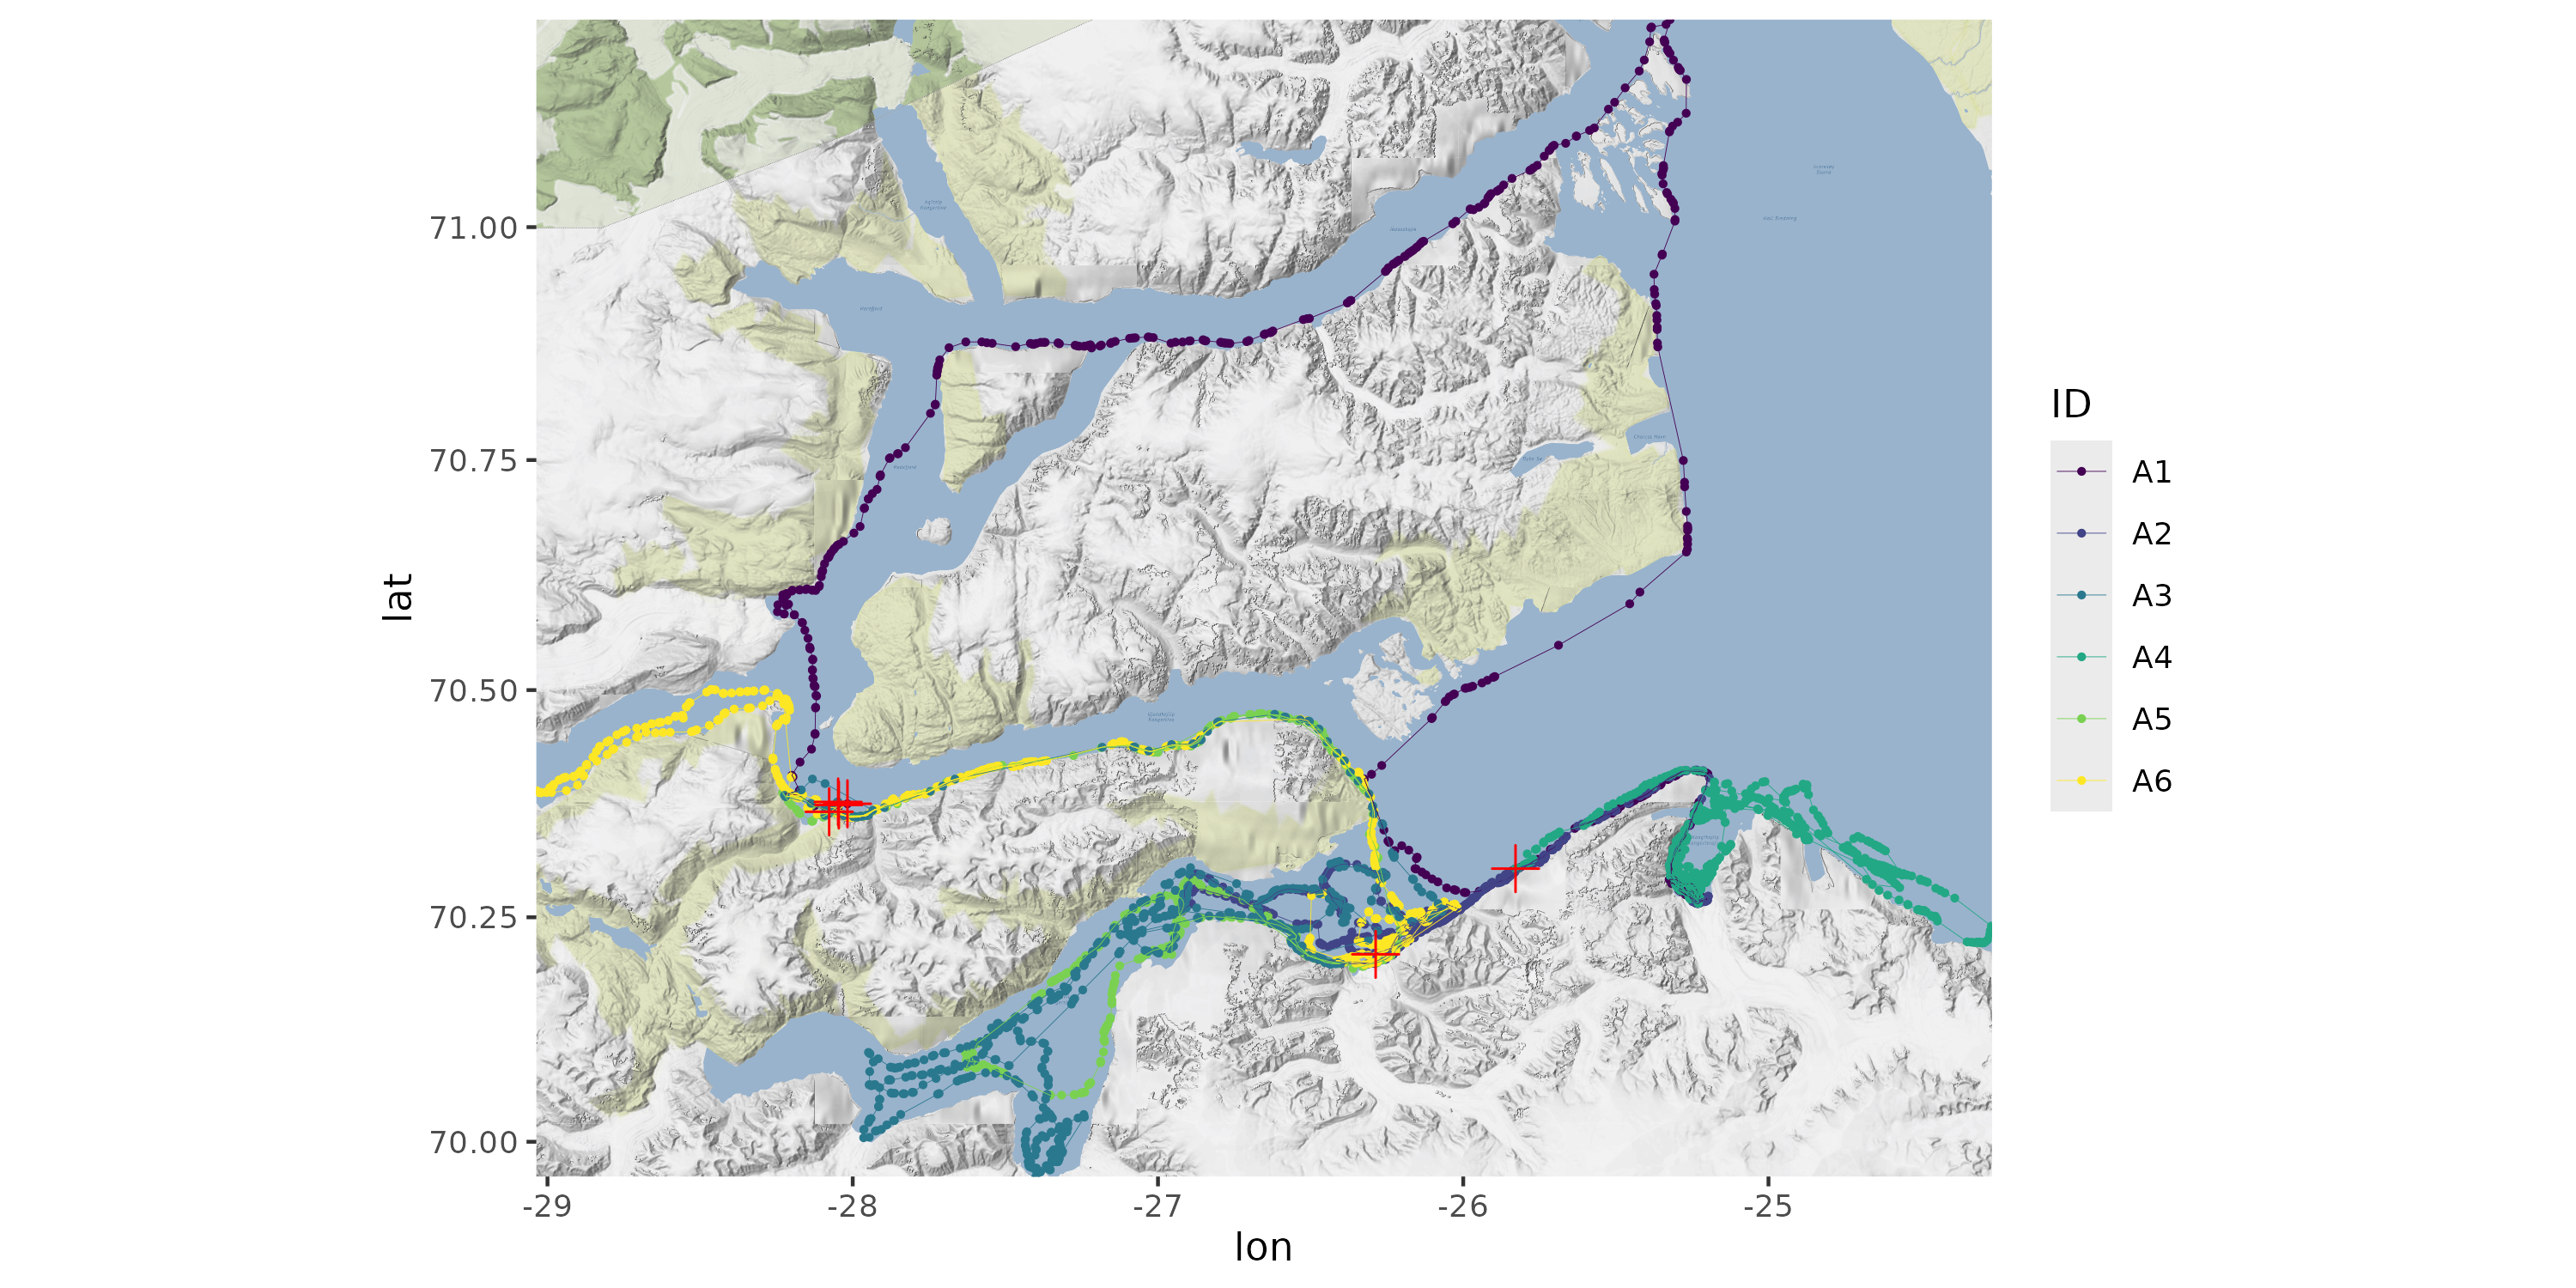
\includegraphics[scale=0.38]{images/data_exploration/tracksAE.png}
		\caption{Tracks during exposure experiments}
	\end{subfigure}
	\caption{Movement data of East Greenland narwhals}
	\label{fig: tracks before and after exposure}
\end{figure}

 All the relevant covariates that are used for the analysis of narwhals movement are summarized in table \ref{tab: covariates}.



\begin{table}[H]
	\centering
	\begin{tabular}{|c|c|p{8cm}|c|}
		\hline
		Covariate & Unit & Description & Domain \\
		\hline
		$D_{ship}(t)$ & km & distance in kilometers between the narwhal and the ship at time $t$ & $\R^+$ \\
		\hline
		$T_{ship}(t)$  & categorical & $0$ when there is no trial, $1$ if it is an intertrial period, and $2$ when it is a trial period & $\{0,1,2\}$\\
		\hline
		$E_{ship}(t)=\frac{1}{D_{ship}(t)}$ & $km^{-1}$ & global exposure level of the narwhal to the ship disturbance at time $t$ & $\R^+$ \\
		\hline
		$E_{ship,I}(t)=\frac{1}{D_{ship}(t)}\mathbb{1}_{T_{ship}(t)=1}$& $km^{-1}$ & intertrial exposure level of the narwhal to the ship disturbance at time $t$ & $\R^+$ \\
		\hline
		$E_{ship,T}(t)=\frac{1}{D_{ship}(t)}\mathbb{1}_{T_{ship}(t)=2}$ & $km^{-1}$ & trial exposure level of the narwhal to the ship disturbance at time $t$. & $\R^+$\\
		\hline
		$D_{shore}(t)$ & km & distance between the narwhal and the nearest point on the shore at time $t$ & $\R^+$ \\
		\hline
		$E_{shore}(t)=\frac{1}{D_{shore}(t)} \1_{D_{shore}(t)<D_0}$ & $km^{-1}$ & global exposure level of the narwhal to the shore at time $t$ & $\R^+$ \\
		\hline
		$\Theta(t)$ & rad & angle between the vector that goes from the nearest shore point to the narwhal's position and the empirical step vector at time $t$  & $[-\pi,\pi]$ \\
		\hline 
	\end{tabular}
	\caption{Summary of the covariates}
	\label{tab: covariates}
\end{table}


\section{Proof of proposition~\ref{prop: transition density}}
\label{section: transition density proof}

\begin{proof}
The velocity process is an Ornstein-Uhlenbeck process. For $t \geq 0$ and $\Delta >0$,
\begin{equation}
	V(t+\Delta)=\exp(-A\Delta) V(t)+ (I_2-\exp(-A\Delta))\mu +\frac{2\nu}{\sqrt{\pi \tau}}\int_{t}^{t+\Delta} \exp(A(s-(t+\Delta))) dW(s)
	\label{eq: RACVM solution}
\end{equation}

It has gaussian transition density with mean 
\begin{equation}
	\E(V(t+\Delta \vert V(t)))=\exp(-A\Delta) V(t)+ (I_2-\exp(-A\Delta))\mu 
\end{equation}
and covariance matrix 
\begin{align*}Var(V(t+\Delta) \vert V(t))&=\frac{4\nu^2}{\pi \tau} \int_{t}^{t+\Delta} \exp(A(s-(t+\Delta))) \exp(A(s-(t+\Delta)))^{\top}\\
	&=\frac{4\nu^2}{\pi \tau} \int_{0}^{\Delta} \exp(-Au) \exp(-Au)^{\top} du 
\end{align*}
Since $\exp(-Au)=\exp(-\frac{u}{\tau}) R_{-\omega u}$, the matrix product  $\exp(-Au) \exp(-Au)^{\top}$ is simply $\exp(-\frac{2u}{\tau}) I_2$. We deduce that the two components of the velocity are independent and have the same variance, written $q_2(\Delta)$ to follow the notations in~\ref{prop: transition density}. The variance is 
\begin{equation}
	q_2(\Delta)=\frac{2\nu^2}{\pi}\left(1-\exp\left(-\frac{2\Delta}{\tau}\right)\right)
\end{equation}
These results are found in \cite{gurarie_correlated_2017}.
In the sequel, we shall use the notation 
\[\zeta(t,s) =\frac{2\nu}{\sqrt{\pi \tau}}\int_{t}^{s} \exp(A(u-s)) dW(u)\] 


\begin{align*}
	X(t+\Delta)&=X(t)+\int_t^{t+\Delta} V(s) ds \mbox{ where } V(s)=\mu+\exp(-A(s-t))(V(t)-\mu)+\zeta(t,s) \\
	&= X(t)+\mu \Delta+\int_t^{t+\Delta} \exp(-A(s-t))(X(t)-\mu) ds +\int_t^{t+\Delta} \zeta(t,s) ds \\
	&= X(t)+\mu \Delta +\int_0^{\Delta} \exp(-As)(X(t)-\mu) ds +\int_t^{t+\Delta} \zeta(t,s) ds \\
	&=X(t)+\mu \Delta + (A^{-1}(V(t)-\mu)-A^{-1}\exp(-A\Delta)(X(t)-\mu))+\int_t^{t+\Delta} \zeta(t,s) ds \\
\end{align*}
Thus, 
\begin{equation}
	X(t+\Delta)=X(t)+\mu \Delta+A^{-1} \left( I_2-\exp(-A\Delta)\right)(V(t)-\mu) +\xi(t,t+\Delta) 
\end{equation}
where $ \xi(t,t+\Delta)=\int_t^{t+\Delta} \zeta(t,s)ds$.
The location process is also gaussian with mean 
\begin{equation}
	\E(X(t+\Delta) \vert V(t),X(t)) =X(t)+\mu \Delta+A^{-1} \left( I_2-\exp(-A\Delta)\right)(V(t)-\mu)
\end{equation}
To get an expression of the covariance matrix, first rewrite

\begin{align*}
	\xi(t,t+\Delta)&=\int_t^{t+÷\Delta} \frac{2 \nu}{\sqrt{\pi \tau}} \left( \int_t^s \exp(-A((u-s))dW(u) \right) ds \\
	&=\frac{2\nu}{\sqrt{\pi\tau}} \int_t^{t+\Delta} \left( \int_u^{t+\Delta} \exp(A(u-s)) ds \right) dW(u)  \\
	&= \frac{2\nu}{\sqrt{\pi \tau}} \int_t^{t+\Delta} (A^{-1}-A^{-1}\exp(A(u-t-\Delta))) dW(u) \\
	&= \frac{2\nu}{\sqrt{\pi \tau}} \int_t^{t+\Delta} A^{-1}(I_2-\exp(A(u-t-\Delta))) dW(u)
\end{align*}

Then use Ito's isometry
\begin{align*}
	Var(X(t+\Delta)\vert X(t),V(t))&=\frac{4 \nu^2}{\pi \tau} \int_{t}^{t+\Delta} A^{-1} (I_2-\exp(A(u-t-\Delta)))(I_2-\exp(A(u-t-\Delta)))^\top A^{-\top} du \\
	&=\frac{4 \nu^2}{\pi \tau} \int_{0}^{\Delta} A^{-1} (I_2-\exp(-Ar))(I_2-\exp(-Ar))^\top A^{-\top} dr
\end{align*}
Now this integral can be computed explicitly since 
\[A^{-1} (I_2-\exp(-Ar))(I_2-\exp(-Ar))^\top A^{-\top}=\frac{1}{C} f(r) I_2 \]
where $f(r)=1-2\exp\left( -\frac{r}{\tau}\right)\cos(\omega r)+\exp\left(\frac{-2r}{\tau}\right)$ and $C=\frac{1}{\tau^2}+\omega^2$.
We obtain that $X_1(t+\Delta)$ and $X_2(t+\Delta)$ are independent and have the same variance, denoted $q_1(\Delta)$.
Writing $\sigma=\frac{2\nu}{\sqrt{\pi \tau}}$, the variance is
\begin{align*}q_1(\Delta)=\frac{\sigma^2}{C} \left( \Delta-2 \frac{\omega \sin(\omega \Delta)-\frac{1}{\tau} \cos(\omega \Delta)}{\frac{1}{\tau^2}+\omega^2 } \exp\left( -\frac{\Delta}{\tau} \right) +\frac{\tau}{2} \left( \frac{\omega^2-\frac{3}{\tau^2}}{\frac{1}{\tau^2}+\omega^2}-\exp\left( -\frac{2\Delta}{\tau}\right)\right) \right)
\end{align*}

Now there is still to compute the covariance between the processes $X$ and $V$ to get the full covariance matrix of $U$. With the same notation as in~\ref{prop: transition density}
\begin{align*}
	\Gamma(\Delta)&=\E\left(\left(\frac{2\nu}{\sqrt{\pi \tau}} \int_t^{t+\Delta} A^{-1}(I_2-\exp(A(u-t-\Delta))) dW(u)\right) \left(\frac{2\nu}{\sqrt{\pi \tau}}\int_{t}^{t+\Delta} \exp(A(s-(t+\Delta))) dW(s)\right)^\top\right) \\
	&= \frac{4\nu^2}{\pi \tau}\int_t^{t+\Delta} A^{-1}(I_2-\exp(A(u-(t+\Delta)))) \exp(A(u-(t+\Delta)))^\top du \\
	&=\frac{4\nu^2}{\pi \tau}\int_0^{\Delta} A^{-1}(I_2-\exp(-Ar)) \exp(-Ar)^\top dr 
\end{align*}
Then, 
\[A^{-1}(I_2-\exp(-Ar)) \exp(-Ar)^\top=\frac{1}{C}\exp\left(-\frac{r}{\tau} \right) \begin{pmatrix} g(r) & h(r) \\ -h(r) & g(r) \end{pmatrix}\]
where $g(r)=\frac{1}{\tau}\left(\cos(\omega r)+\exp\left( -\frac{r}{\tau} \right)\right) -\omega \sin(\omega r)$ and $h(r)=-\frac{1}{\tau}\sin(\omega r)+\omega\left(\cos(\omega r)-\exp\left( -\frac{r}{ \tau}\right)\right)$.
Eventually we get
\[
\gamma_1(\Delta)=\frac{\sigma^2}{2C}\left( 1+\exp\left( -\frac{2\Delta}{\tau}\right)-2\exp\left( -\frac{\Delta}{\tau}\right)-2\exp\left( -\frac{\Delta}{\tau}\right) \cos(\omega \Delta)\right)
\]
\[\gamma_2(\Delta)=\frac{\sigma^2}{C}\left( \exp\left( -\frac{\Delta}{\tau}\right) \sin(\omega \Delta)-\frac{\omega \tau}{2} \left(1-\exp\left( -2 \frac{\Delta}{\tau}\right) \right)\right)\]

In the specific case $\omega=0$, we obtain $C=\frac{1}{\tau^2}$ and the variance of the location process $X$ becomes 
\[q_1(\Delta)=\sigma^2 \tau^2\left( \Delta +2\tau\exp\left( -\frac{\Delta}{\tau}\right)+\frac{\tau}{2}\left( -3 -\exp\left( -\frac{2\Delta}{\tau}\right) \right)\right)
\]
Writing $\beta=\frac{1}{\tau}$ and reorganizing the terms, we obtain
\begin{equation}q_1(\Delta)=\frac{\sigma^2}{\beta^2}\left(\Delta -2 \frac{1-\exp(-\beta \Delta)}{\beta}+\frac{1-e^{-2\beta \Delta}}{2\beta}\right)
\end{equation}
This result match equation $(6)$ in \cite{johnson_continuoustime_2008}. Similarly, in the case $\omega=0$, we get $\gamma_2=0$ and the expression for $\gamma_1$ match equation $(7)$ in \cite{johnson_continuoustime_2008}.

\end{proof}

\section{More results about the standard RACVM}
\subsection{Stationary distribution}

If $v(0) \sim \mathcal{N}\left(\mu,\frac{2\nu^2}{\pi} I_2\right)$ then for all $t \geq 0$, $v(t) \sim \mathcal{N}\left(\mu,\frac{2\nu^2}{\pi} I_2\right)$

\subsection{Distribution of the velocity norm and phase}
 The order of magnitude of the parameter $\nu$ is similar to the overall mean empirical velocity norm. The distribution of the phase angle $\Phi$ of the velocity is derived in \cite{pawula_distribution_1982}.
When $\mu=0$, this distribution is uniform over $[-\pi,\pi]$. Hence, taking a look at the histograms of the phase angle of the data can help to assess whether a non zero mean velocity is necessary in the model or not.

Suppose that $t\geq \frac{3}{\beta}$ so that the velocity has reached its stationary distribution
\begin{align*}
	&v_1(t) \sim \mathcal{N}\left(\mu_1, \frac{2\nu^2}{\pi}\right) \\
	&v_2(t) \sim \mathcal{N}\left(\mu_2, \frac{2\nu^2}{\pi}\right)
\end{align*}

\begin{figure}[H]
	\centering
	\begin{tikzpicture}
		% Draw axes
		\draw[->] (-1,0) -- (5,0) node[right] {$x$};
		\draw[->] (0,-1) -- (0,5) node[above] {$y$};
		
		% Draw point at (3,4) with circle
		\fill (3,4) circle (2pt);
		\draw[blue,dashed] (3,4) circle (1.5);
		
		%Draw vectors
		\draw[->,dotted,red] (-0,0) -- (3.5,3.5) node[right] {$v(t)$};
		\draw[->,dotted,red] (0,0) -- (2.6,4.2) node[above] {$v(t')$};
		% Add node with text $\mu$
		\node at (3,4) [above right] {$\mu$};
		
		% Add node beside the circle with text $\frac{\sigma^2}{2\beta}$
		\node[blue] at (4.5,3) [anchor=west] {$\frac{\sigma^2}{2\beta}$};
	\end{tikzpicture}
\end{figure}
Thus, $ \vert \vert v(t) \vert \vert$ follows a \href{https://en.wikipedia.org/wiki/Rice_distribution}{Rice distribution} with mean parameter $\vert \vert \mu \vert \vert$ and variance parameter $\frac{2\nu^2}{\pi}$. Its probability density function is thus defined by
\[\forall x \geq 0, \quad f(x)= \frac{\pi}{2\nu^2}x \exp\left(-\frac{\pi (x^2+ \vert \vert \mu \vert \vert^2)}{4\nu^2}\right) I_{0}\left(   \frac{\pi}{2\nu^2}\times \vert \vert \mu \vert \vert x \right)\]
where $I_0$ is a modified Besssel function of the first kind defined such that 
\[\forall y  \in \R, \quad I_0(y)=\sum_{m=0}^{+\infty} \frac{1}{m!^2}\left(\frac{y}{2}\right)^{2m}\]
Its moments can be expressed with
\[\E\left(\vert \vert v(t) \vert \vert\right)=\sqrt{\frac{2}{\pi}}\nu \times \sqrt{\frac{\pi}{2}} L_{\frac{1}{2}} \left( -\frac{\pi}{4\nu^2} \vert \vert \mu \vert \vert ^2 \right)\]

Here, $L_{\frac{1}{2}}(x)=e^{\frac{x}{2}} \left( (1-x) I_0\left( -\frac{x}{2}\right)-xI_1\left( -\frac{x}{2}\right)\right)$ with $I_1(y)=\sum_{m=0}^{+\infty} \frac{1}{m!(m+1)!}\left(\frac{y}{2}\right)^{2m+1}$.\\

In the case $\mu=(0,0)$, the mean velocity norm is simply 
\[\E(\vert \vert v(t) \vert \vert)=\nu L_{\frac{1}{2}}(0)=\nu I_{0}(0)=\nu\]
This result can be used to choose initial value of the parameter $\nu$ based on the mean observed empirical velocity.

Then, in the plane, $v(t)$ can be thought of as a complex random variable $v(t)=v_1(t)+iv_2(t)$ that has complex normal distribution with mean $\mu_1+i\mu_2$, variance $\E\left((v(t)-\E(v(t)))\overline{(v(t)-\E(v(t)))}\right)=\frac{4\nu^
	2}{\pi}$ and pseudo-variance $\E\left((v(t)-\E(v(t)))^2\right)=0$. Thus, $v(t)$ has a circular symmetric normal distribution with mean $\mu_1+i\mu_2=\vert \vert \mu \vert \vert e^{i\theta}$ where $\theta=\arctan(\mu_2,\mu_1) \in [-\pi, \pi]$ and variance $\frac{\sigma^2}{\beta}$.
Denote $\Phi=\arctan(v_2(t),v_1(t)) \in [-\pi, \pi]$ the phase angle of $v(t)$.
According to \cite{letzepis_von_2015}, the distribution of $\Phi$ is 
\[\forall \phi \in [-\pi,\pi], \quad f_{\Phi}(\phi)=\frac{e^{-\frac{\beta \vert \vert \mu \vert \vert^2}{2\sigma^2}}}{2\pi} +\frac{\sqrt{\beta} \vert \vert \mu \vert \vert}{2\sigma\sqrt{2\pi}} \cos(\phi-\theta)e^{-\frac{\beta\vert \vert \mu \vert \vert^2 \sin^2(\phi-\theta)}{2\sigma^2}} \times \left(1+\erf\left(\frac{\beta^{\frac{1}{4}}\vert \vert \mu \vert \vert \cos(\phi-\theta)}{\sqrt{2\sigma}}\right)\right)\]
where $\beta=\frac{1}{\tau}$, $\sigma=\frac{2\nu}{\sqrt{\pi \tau}}$ and $\erf$ is the Gauss error function defined by 
\[\forall z \in \R, \quad \erf(z)=\frac{2}{\sqrt{\pi}} \int_0^z e^{-t^2} dt\]
When $\mu=0$, this simplifies to a uniform distribution over $[-\pi,\pi]$.\\
%plot of the function for non zero mu


\subsection{Velocity autocovariance function}

Suppose that $v(0)$ has the stationary distribution.The autocovariance function is the expected dot product of the velocity vectors over different lags.

\[\mathbb{E}(\langle v(t), v(t+\Delta) \rangle =Cov(v_1(t)v_1(t+\Delta))+Cov(v_2(t),v_2(t+\Delta))+\mathbb{E}(v_1(t)) \mathbb{E}(v_1(t+\Delta))+\mathbb{E}(v_2(t)) \mathbb{E}(v_2(t+\Delta))\]

Therefore, the velocity autocovariance function is 

\begin{equation}
	\mathbb{E}(\langle v(t), v(t+\Delta) \rangle )=\frac{4\nu^2}{\pi} \cos(\omega \Delta) e^{-\frac{\Delta}{\tau}}+\vert \vert \mu \vert \vert^2
	\label{eq: RACVM autocovariance function}
\end{equation}


\end{document}